\documentclass[a4paper,11pt]{article}
\usepackage[a4paper]{geometry}
\usepackage[utf8]{inputenc}
\title{Advanced Solid State Physics Problem Notes \\ DTU Course 10305}
\author{Lecturer: \emph{Kristian Thygesen}\\
Contributors: \emph{Asbjoern Moltke, Rasmus Eilkaer, Ulrik Leffers, Victor Elkjaer}}
\date{Fall 2018}

%%%%%%%%%%%%%%%%%%%%%%%%%%%%%%%%%%%%%%%%%%
%            Packages                    %
%%%%%%%%%%%%%%%%%%%%%%%%%%%%%%%%%%%%%%%%%%
\usepackage{amsfonts,amsmath,amssymb} % Math symbols form American Mathematical Society
\usepackage[english]{babel} 
\usepackage{textcomp}
\usepackage{bm}
\usepackage{makeidx}
\usepackage{graphicx}
\usepackage{amsthm}
\usepackage{enumerate}%http://ctan.org/pkg/enumerate


%%%%%%%%%%%%%%%%%%%%%%%%%%%%%%%%%%%%%%%%%%
%               Newcommands              %
%%%%%%%%%%%%%%%%%%%%%%%%%%%%%%%%%%%%%%%%%%

% BATMAN
\newcommand{\batmanPic}[1]{
    \begin{tikzpicture}[baseline=0em, scale=#1]
        \draw[fill,black]   (-0.25,1.48) .. controls (-0.1,1.5) and (0.1,1.5) .. (0.25,1.48) -- (0.35,1.92) .. controls (0.425,1.8) and (0.41,1.3) .. (0.45,1.2) .. controls (0.6,1.05) and (1.96,1.05) .. (1.98,2.08) -- (5.93,2.08) .. controls (4.2,1.45) and (4,0.3) .. (4.2,-0.28) .. controls (2.4,-0.09) and (0.4,-0.5) .. (0,-2.052) .. controls (-0.4,-0.5) and (-2.4,-0.09) .. (-4.2,-0.28) .. controls (-4,0.3) and (-4.2,1.45) .. (-5.93,2.08) -- (-1.98,2.08) .. controls (-1.96,1.05) and (-0.6,1.05) .. (-0.45,1.2) .. controls (-0.41,1.3) and (-0.425,1.8) .. (-0.35,1.92) -- (-0.25,1.48);
    \end{tikzpicture}
    
} % End of \batman command
\newcommand{\batman}{\batmanPic{0.05}}
\renewcommand\qedsymbol{\batman}

\newcommand{\crea}[2]{\hat{#1}_{#2}^{\dagger}}
\newcommand{\anni}[2]{\hat{#1}_{#2}}
% SMART COMMANDS FOR THIS PROJECT
\DeclareMathOperator*{\argmin}{\arg\!\min}
\DeclareMathOperator*{\argmax}{\arg\!\max}
\newcommand{\Lnorm}[1]{$L_{#1}$-norm}
\newcommand{\R}{\mathbb{R}}
\newcommand{\C}{\mathbb{C}}
\newcommand{\bsw}{\boldsymbol{w}}
\newcommand{\cov}{\mathrm{c\hat{o}v}}
\newcommand{\covm}{\boldsymbol{\Sigma}}
\newcommand{\curlyb}[1]{\left\{ {#1} \right\}}
\newcommand{\Egeneral}{E_{\mathcal{M}}^{\mathrm{gen}}}
\newcommand{\Dtrain}{\mathcal{D}_{\mathrm{train}}}
\newcommand{\Dtest}{\mathcal{D}_{\mathrm{test}}}
\newcommand{\EM}[1]{\hat{E}_{\mathcal{M}}^{\mathrm{#1}}}
\newcommand{\EMss}[2]{E_{{\mathcal{M}#1}}^{{\mathrm{#2}}}}
\newcommand{\FM}[1]{f_{\mathcal{M}}\qty(#1)}
\newcommand{\calDss}[2]{\mathcal{D}_{{#1}}^{{\mathrm{#2}}}}
\newcommand{\RMSE}{\mathrm{RMSE}}
\newcommand{\hadd}{h_{add}}
\newcommand{\hast}{h^{\ast}}
\newcommand{\expe}[1]{\mathrm{e}^{{#1}}}


% NEW THEOREM ENVIRONMENT: Exercise
\usepackage{mdframed}
\newtheorem{mdexercise}{Exercise}[subsection]
\newtheorem{solution}{Solution}[subsection]
\newenvironment{exercise}
  {\begin{mdframed}[backgroundcolor=black!5]\begin{mdexercise}}
  {\end{mdexercise}\end{mdframed}}



% SPACINGS
\newcommand{\linie}{\underline{\makebox[\textwidth]{}}}
\newcommand{\spacer}{\rule[-2mm]{0mm}{6mm}}
\newcommand{\notop}{{{}_{}}}
\newcommand{\ontop}[1]{{{#1}_{}}}
%
% LITERAL ABBREVIATIONS
\newcommand{\ie}{i.e.}
\newcommand{\eg}{e.g.}
\newcommand{\etc}{\textit{etc.}}
\newcommand{\etal}{\textit{et~al.}}
\newcommand{\MICDTU}{DTU Nanotech}
%
% MATH SYMBOLS
\renewcommand{\vec}[1]{\bm{#1}}
\newcommand{\ee}{\mathrm{e}}
\newcommand{\ii}{\mathrm{i}}
\newcommand{\dm}{\mathrm{d}}
\newcommand{\sgn}{\mathrm{sgn}}
\newcommand{\sm}{\!-\!}
\newcommand{\sP}{\!+\!}
\newcommand{\im}{\mathrm{Im}}
\newcommand{\re}{\mathrm{Re}}
\newcommand{\krondel}[2]{\delta^\notop_{#1 #2}}
\newcommand{\Tr}{\mathrm{Tr}}
\newcommand{\ion}{\ii\omega^\notop_n}
\newcommand{\iot}{\ii\omega t}
\newcommand{\taun}{\tau^\notop}
\newcommand{\lam}{\lambda}
\newcommand{\lamn}{\lambda^{{}}}
\newcommand{\limit}[2]{\mathop{\longrightarrow}_{#1 \rightarrow #2}}
\newcommand{\gamn}{\gamma^{{}}}
\newcommand{\nun}{\nu^\notop}
\newcommand{\ve}{\varepsilon}
\newcommand{\ven}{\ve^\notop}
\newcommand{\xin}{\xi^\notop}
\newcommand{\zetan}{\zeta^\notop}
\newcommand{\pp}{\partial^{{}}}
\newcommand{\ppsqr}{\partial^{\,2_{}}}
\newcommand{\nablabf}{\boldsymbol{\nabla}}
\newcommand{\nablabfn}{\boldsymbol{\nabla}^\notop}
\newcommand{\Lapl}{\nabla^2}
\newcommand{\nablasqr}{\nabla^2}
\newcommand{\rot}{\nablabf\times}
\newcommand{\divop}{\nablabf\scap}
%
% MATH STYLE
\newcommand{\scap}{\!\cdot\!}
\newcommand{\intd}[1]{{\int\!\dm#1\: }}
\newcommand{\inttau}[1]{{\int_0^\beta\!d\tauno_{#1}\: }}
\newcommand{\dpst}{\displaystyle}
\newcommand{\scst}{\scriptstyle}
\newcommand{\scscst}{\scriptscriptstyle}
\newcommand{\fracsmall}[2]{\mbox{$\frac{#1}{#2}$}}
\newcommand{\sqrtsmall}[1]{\mbox{$\sqrt{#1}$}}
\newcommand{\half}{\fracsmall{1}{2}}
\newcommand{\third}{\fracsmall{1}{3}}
\newcommand{\quarter}{\fracsmall{1}{4}}
%
% BOLD SYMBOLS
\newcommand{\AAA}{\vec{A}}
\newcommand{\AAn}{\vec{A}^\notop}
\newcommand{\Ann}{A^\notop}
\newcommand{\aaa}{\vec{a}}
\newcommand{\aan}{\vec{a}^\notop}
\newcommand{\ann}{a^\notop}
\newcommand{\asqr}{a^{2_{}}}
\newcommand{\BBB}{\vec{B}}
\newcommand{\BBn}{\vec{B}^\notop}
\newcommand{\Bnn}{B^\notop}
\newcommand{\bbb}{\vec{b}}
\newcommand{\bbn}{\vec{b}^\notop}
\newcommand{\bnn}{b^\notop}
\newcommand{\bsqr}{b^{2_{}}}
\newcommand{\CCC}{\vec{C}}
\newcommand{\CCn}{\vec{C}^\notop}
\newcommand{\CD}{C^\notop_\mathrm{D}}
\newcommand{\Cs}{C^\notop_\mathrm{s}}
\newcommand{\ccc}{\vec{c}}
\newcommand{\ccn}{\vec{c}^\notop}
\newcommand{\cnn}{c^\notop}
\newcommand{\DDD}{\vec{D}}
\newcommand{\DDn}{\vec{D^\notop}}
\newcommand{\ddd}{\vec{d}}
\newcommand{\ddn}{\vec{d^\notop}}
\newcommand{\EEE}{\vec{E}}
\newcommand{\EEn}{\vec{E^\notop}}
\newcommand{\Enn}{E^\notop}
\newcommand{\eee}{\vec{e}}
\newcommand{\een}{\vec{e}^\notop}
\newcommand{\FFF}{\vec{F}}
\newcommand{\FFn}{\vec{F}^\notop}
\newcommand{\Fnn}{F^\notop}
\newcommand{\FFFe}{\vec{F}^\notop_\mathrm{el}}
\newcommand{\fff}{\vec{f}}
\newcommand{\ffn}{\vec{f}^\notop}
\newcommand{\fnn}{f^\notop}
\newcommand{\fffe}{\vec{f}^\notop_\mathrm{el}}
\newcommand{\GGn}{\vec{G}}
\newcommand{\GGG}{\vec{G}^\notop}
\newcommand{\ggn}{\vec{g}^\notop}
\newcommand{\gnn}{g^\notop}
\newcommand{\HHH}{\vec{H}}
\newcommand{\HHn}{\vec{H}^\notop}
\newcommand{\iii}{\vec{i}}
\newcommand{\iin}{\vec{i}^\notop}
\newcommand{\JJJ}{\vec{J}}
\newcommand{\JJn}{\vec{J}^\notop}
\newcommand{\Jnn}{J^\notop}
\newcommand{\JJJe}{\vec{J}^\notop_\mathrm{el}}
\newcommand{\JJJti}{\vec{\tilde{J}}}
\newcommand{\JJnti}{\vec{\tilde{J}}^\notop}
\newcommand{\JJdiff}{\vec{J}^{\mathrm{diff}_{}}}
\newcommand{\Jdiff}{J^{\mathrm{diff}_{}}}
\newcommand{\JJext}{\vec{J}^{{}}_{\mathrm{ext}}}
\newcommand{\JJmag}{\vec{J}^{{}}_{\mathrm{mag}}}
\newcommand{\JJheat}{\vec{J}^{{}}_{\mathrm{heat}}}
\newcommand{\Jheat}{J^{{}}_{\:\mathrm{heat}}}
\newcommand{\JJhcond}{\vec{J}^\mathrm{cond}_\mathrm{heat}}
\newcommand{\Jhcond}{J^{\:\mathrm{cond}}_{\:\:\mathrm{heat}}}
\newcommand{\JJhconv}{\vec{J}^\mathrm{conv}_\mathrm{heat}}
\newcommand{\Jhconv}{J^{\:\mathrm{conv}}_{\:\:\mathrm{heat}}}
\newcommand{\kkk}{\vec{k}}
\newcommand{\kkn}{\vec{k}^\notop}
\newcommand{\knn}{k^\notop}
\newcommand{\ksqr}{k^{2_{}}}
\newcommand{\KKK}{\vec{K}}
\newcommand{\KKn}{\vec{K}^\notop}
\newcommand{\MMM}{\vec{M}}
\newcommand{\MMn}{\vec{M}^\notop}
\newcommand{\mmm}{\vec{m}}
\newcommand{\mmn}{\vec{m}^\notop}
\newcommand{\nnn}{\vec{n}}
\newcommand{\nnnn}{\vec{n}^\notop}
\newcommand{\PPP}{\vec{P}}
\newcommand{\PPn}{\vec{P}^\notop}
\newcommand{\ppp}{\vec{p}}
\newcommand{\ppn}{\vec{p}^\notop}
\newcommand{\pnn}{p^\notop}
\newcommand{\QQQ}{\vec{Q}}
\newcommand{\QQn}{\vec{Q}^\notop}
\newcommand{\Qnn}{Q^\notop}
\newcommand{\qqq}{\vec{q}}
\newcommand{\qqn}{\qqq^\notop}
\newcommand{\RRR}{\vec{R}}
\newcommand{\RRn}{\RRR^\notop}
\newcommand{\Rnn}{R^\notop}
\newcommand{\rrr}{\vec{r}}
\newcommand{\rrn}{\rrr^\notop}
\newcommand{\rij}{r^\notop_{ij}}
\newcommand{\sss}{\vec{s}}
\newcommand{\ssn}{\sss^\notop}
\newcommand{\snn}{s^\notop}
\newcommand{\ssqr}{s^{2_{}}}
\newcommand{\Tnn}{{T}^\notop}
\newcommand{\uuu}{\vec{u}}
\newcommand{\uun}{\vec{u}^\notop}
\newcommand{\unn}{{u}^\notop}
\newcommand{\VVV}{\vec{V}}
\newcommand{\VVn}{\vec{V}^\notop}
\newcommand{\Vnn}{{V}^\notop}
\newcommand{\VLJ}{{V}^\notop_\mathrm{LJ}}
\newcommand{\vvv}{\vec{v}}
\newcommand{\vvn}{\vec{v}^\notop}
\newcommand{\vnn}{{v}^\notop}
\newcommand{\www}{\vec{w}}
\newcommand{\wwn}{\vec{w}^\notop}
\newcommand{\wnn}{{w}^\notop}
\newcommand{\wdd}{w^{{}}_\mathrm{d}}
\newcommand{\xxx}{\vec{x}}
\newcommand{\xxn}{\xxx^\notop}
\newcommand{\XXX}{\vec{X}}
\newcommand{\xnn}{x^\notop}
\newcommand{\yyy}{\vec{y}}
\newcommand{\Znn}{Z^\notop}
\newcommand{\znn}{z^\notop}
\newcommand{\zerovec}{\boldsymbol{0}}
%
% PHYSICS SYMBOLS
\newcommand{\calA}{\mathcal{A}}
\newcommand{\calC}{\mathcal{C}}
\newcommand{\calCn}{\mathcal{C}^{{}}}
\newcommand{\calD}{\mathcal{D}}
\newcommand{\calDn}{\mathcal{D}^{{}}}
\newcommand{\calO}{\mathcal{O}}
\newcommand{\calP}{\mathcal{P}}
\newcommand{\calPO}{\mathcal{P}^{{}}_0}
\newcommand{\calPs}{\mathcal{P}^{{}}_\mathrm{s}}
\newcommand{\calPf}{\mathcal{P}^{{}}_\mathrm{f}}
\newcommand{\calR}{\mathcal{R}}
\newcommand{\calT}{\mathcal{T}}
\newcommand{\calV}{\mathcal{V}}
\newcommand{\area}{\mathcal{A}}
\newcommand{\aI}{{a^{{}}_1}}
\newcommand{\aIsqr}{{a^{2_{}}_1}}
\newcommand{\aIcub}{{a^{3_{}}_1}}
\newcommand{\aII}{{a^{{}}_2}}
\newcommand{\aIIsqr}{{a^{2_{}}_2}}
\newcommand{\aIIcub}{{a^{3_{}}_2}}
\newcommand{\aB}{{a^\notop_0}}
\newcommand{\ath}{{a^\notop_\mathrm{th}}}
\newcommand{\ap}{{a^\notop_\mathrm{p}}}
\newcommand{\aexp}{{a^\notop_\mathrm{exp}}}
\newcommand{\alphap}{\alpha^{{}}_\mathrm{p}}
\newcommand{\aeta}{{\alpha^\notop_\eta}}
\newcommand{\akap}{{\alpha^\notop_\kappa}}
\newcommand{\arho}{{\alpha^\notop_\rho}}
\newcommand{\aetasqr}{{\alpha^{2_{}}_\eta}}
\newcommand{\akapsqr}{{\alpha^{2_{}}_\kappa}}
\newcommand{\arhosqr}{{\alpha^{2_{}}_\rho}}
\newcommand{\BO}{\textit{Bo}}
\newcommand{\CCD}{C^{{}}_\mathrm{D}}
\newcommand{\Chyd}{C^{{}}_\mathrm{hyd}}
\newcommand{\CA}{\textit{Ca}}
\newcommand{\CCa}{C^{{}}_\alpha}
\newcommand{\cca}{c^{{}}_\alpha}
\newcommand{\ca}{c^{{}}_\mathrm{a}}
\newcommand{\casqr}{c^{2_{}}_\mathrm{a}}
\newcommand{\cm}{c^{{}}_\mathrm{m}}
\newcommand{\cmO}{c^{(0)_{}}_\mathrm{m}}
\newcommand{\cmI}{c^{(1)_{}}_\mathrm{m}}
\newcommand{\cmII}{c^{(2)_{}}_\mathrm{m}}
\newcommand{\cmi}{c^{(i)_{}}_\mathrm{m}}
\newcommand{\co}{c^{{}}_\mathrm{o}}
\newcommand{\cp}{c^{{}}_\mathrm{p}}
\newcommand{\cpm}{c^{{}}_\pm}
\newcommand{\cpp}{c^{{}}_+}
\newcommand{\cmm}{c^{{}}_-}
\newcommand{\Cth}{C^\notop_\mathrm{th}}
\newcommand{\dktwopicubed}{\frac{d\kkk}{\twopicubed}}
\newcommand{\Deln}{\Delta^\notop}
\newcommand{\Dth}{D^\notop_\mathrm{th}}
\newcommand{\Ekin}{E^{{}}_\mathrm{kin}}
\newcommand{\Etot}{E_\mathrm{tot}}
\newcommand{\ffe}{\fff^{{}}_\mathrm{el}}
\newcommand{\FC}{\mathcal{F}}
\newcommand{\FFFdip}{\FFF^{{}}_\mathrm{dip}}
\newcommand{\FFFDEP}{\FFF^{{}}_\mathrm{DEP}}
\newcommand{\FFFdrag}{\FFF^{{}}_\mathrm{drag}}
\newcommand{\Fimp}{F^{{}}_\mathrm{imp}}
\newcommand{\GC}{G}
\newcommand{\GCn}{G^{{}}}
\newcommand{\Ghyd}{G^{{}}_\mathrm{hyd}}
\newcommand{\hc}{h^{{}}_\mathrm{c}}
\newcommand{\hf}{h^{{}}_\mathrm{f}}
\newcommand{\Dh}{\Delta h}
\newcommand{\IO}{I^{{}}_0}
\newcommand{\Is}{I^{{}}_\mathrm{s}}
\newcommand{\If}{I^{{}}_\mathrm{f}}
\newcommand{\Ith}{I^\notop_\mathrm{th}}
\newcommand{\Ieo}{I^\notop_\mathrm{eo}}
\newcommand{\Ieocond}{I^{\textrm{cond}_{}}_\mathrm{eo}}
\newcommand{\Ieoconv}{I^{\textrm{conv}_{}}_\mathrm{eo}}
\newcommand{\Ipconv}{I^{\textrm{conv}_{}}_\mathrm{p}}
\newcommand{\kB}{{k^\notop_\mathrm{B}}}
\newcommand{\kBT}{{k^\notop_\mathrm{B} T}}
\newcommand{\Lc}{L^{{}}_\mathrm{c}}
\newcommand{\Lx}{L^{{}}_x}
\newcommand{\Ly}{L^{{}}_y}
\newcommand{\Lz}{L^{{}}_z}
\newcommand{\elln}{\ell^\notop}
\newcommand{\elli}{{\ell^{{}}_\mathrm{i}}}
\newcommand{\ello}{{\ell^{{}}_\mathrm{o}}}
\newcommand{\elld}{{\ell^{{}}_\mathrm{d}}}
\newcommand{\ellc}{\ell^{{}}_\mathrm{c}}
\newcommand{\lcap}{\ell^{{}}_\mathrm{cap}}
\newcommand{\lcapsqr}{\ell^{2_{}}_\mathrm{cap}}
\newcommand{\len}{\mathcal{L}}
\newcommand{\nre}{n^{{}}_\mathrm{re}}
\newcommand{\nim}{n^{{}}_\mathrm{im}}
\newcommand{\nnp}{n^{+_{}}}
\newcommand{\nnm}{n^{-_{}}}
\newcommand{\npm}{n^{\pm_{}}}
\newcommand{\nin}{n^\notop_\mathrm{in}}
\newcommand{\nout}{n^\notop_\mathrm{out}}
\newcommand{\Ps}{P^{{}}_\mathrm{s}}
\newcommand{\pc}{{p^{{}}_\mathrm{c}}}
\newcommand{\peo}{p^\notop_\mathrm{eo}}
\newcommand{\phs}{p^{{}}_\mathrm{hs}}
\newcommand{\ptot}{p^{{}}_\mathrm{tot}}
\newcommand{\pimp}{p^{{}}_\mathrm{imp}}
\newcommand{\pL}{{p^{{}}_\mathrm{L}}}
\newcommand{\pR}{{p^{{}}_\mathrm{R}}}
\newcommand{\pii}{{p^{{}}_{\,\mathrm{i}}}}
\newcommand{\piiI}{{p^{{}}_{\,\mathrm{i},1}}}
\newcommand{\piiII}{{p^{{}}_{\,\mathrm{i},2}}}
\newcommand{\poo}{{p^{{}}_\mathrm{o}}}
\newcommand{\pdd}{{p^{{}}_\mathrm{d}}}
\newcommand{\pww}{{p^{{}}_\mathrm{w}}}
\newcommand{\Dp}{\Delta p}
\newcommand{\Dpn}{\Delta p^{{}}}
\newcommand{\dpb}{\Delta p^{{}}_\mathrm{b}}
\newcommand{\Dpb}{\Delta p^{{}}_\mathrm{b}}
\newcommand{\pclog}{p^{{}}_\mathrm{clog}}
\newcommand{\Dpsurf}{\Delta p^{{}}_\mathrm{surf}}
\newcommand{\DPsurf}{\Delta p^{{}}_\mathrm{surf}}
\newcommand{\DP}{\Delta P}
\newcommand{\Peth}{\PE^{{}}_\mathrm{th}}
\newcommand{\PE}{\textit{P\'e}}
\newcommand{\Qc}{Q^{{}}_\mathrm{c}}
\newcommand{\Qcav}{Q^\notop_\mathrm{c}}
\newcommand{\Qeo}{Q^\notop_\mathrm{eo}}
\newcommand{\QeoS}{Q^{*_{}}_\mathrm{eo}}
\newcommand{\Qexp}{Q^\notop_\mathrm{exp}}
\newcommand{\Qmass}{Q^\notop_\mathrm{mass}}
\newcommand{\QmassO}{Q^\notop_{\textrm{mass},0}}
\newcommand{\Qtot}{Q^\notop_\mathrm{tot}}
\newcommand{\Qp}{Q^\notop_\mathrm{p}}
\newcommand{\Qii}{{Q^{{}}_\mathrm{i}}}
\newcommand{\Qoo}{{Q^{{}}_\mathrm{o}}}
\newcommand{\Qdd}{{Q^{{}}_\mathrm{d}}}
\newcommand{\Qth}{Q^\notop_\mathrm{th}}
\newcommand{\QthS}{Q^{*_{}}_\mathrm{th}}
\newcommand{\RE}{\textit{Re}}
\newcommand{\RcI}{R^{\mathrm{c}_{}}_1}
\newcommand{\RcII}{R^{\mathrm{c}_{}}_2}
\newcommand{\Rh}{R^{{}}_\mathrm{hyd}}
\newcommand{\RhS}{R^{*_{}}_\mathrm{hyd}}
\newcommand{\Rhyd}{R^{{}}_\mathrm{hyd}}
\newcommand{\RhydS}{R^{*_{}}_\mathrm{hyd}}
\newcommand{\Rhydp}{R^{\textrm{p}_{}}_\mathrm{hyd}}
\newcommand{\Rhydexp}{R^{\textrm{exp}_{}}_\mathrm{hyd}}
\newcommand{\Rth}{R^\notop_\mathrm{th}}
\newcommand{\DS}{\Delta S}
\newcommand{\Tg}{T^{{}}_\mathrm{g}}
\newcommand{\Tc}{T^{{}}_\mathrm{c}}
\newcommand{\Dt}{\Delta t}
\newcommand{\DT}{\Delta T}
\newcommand{\tacc}{\tau^{{}}_\mathrm{acc}}
\newcommand{\tadv}{\tau^{{}}_\mathrm{adv}}
\newcommand{\tcap}{\tau^{{}}_\mathrm{cap}}
\newcommand{\timp}{\tau^{{}}_\mathrm{imp}}
\newcommand{\tdiff}{\tau^{{}}_\mathrm{diff}}
\newcommand{\tdiffa}{\tau^{\textrm{ax}_{}}_\mathrm{diff}}
\newcommand{\tdiffr}{\tau^{\textrm{rad}_{}}_\mathrm{diff}}
\newcommand{\tconv}{\tau^{{}}_\mathrm{conv}}
\newcommand{\tconva}{\tau^{{L^{{}}_{}}}_\mathrm{conv}}
\newcommand{\tconvr}{\tau^{{a^{{}}_{}}}_\mathrm{conv}}
\newcommand{\tRC}{\tau^{{}}_{RC}}
\newcommand{\vol}{\mathcal{V}}
\newcommand{\vg}{\vnn_\mathrm{g}}
\newcommand{\veo}{\vnn_\mathrm{eo}}
\newcommand{\vvvwall}{\vvn_\mathrm{wall}}
\newcommand{\DV}{\Delta V}
\newcommand{\xc}{{x^{{}}_\mathrm{c}}}
\newcommand{\xcm}{{x^{{}}_\mathrm{cm}}}
\newcommand{\xL}{{x^{{}}_\mathrm{L}}}
\newcommand{\xR}{{x^{{}}_\mathrm{R}}}
\newcommand{\Dx}{\Delta x}
\newcommand{\Dy}{\Delta y}
\newcommand{\Dz}{\Delta z}
\newcommand{\zc}{{z^{{}}_\mathrm{c}}}
\newcommand{\deltan}{\delta^\notop}
\newcommand{\eps}{\epsilon}
\newcommand{\epsn}{\epsilon^{{}}}
\newcommand{\epss}{\epsilon^\notop_\mathrm{s}}
\newcommand{\epsO}{\epsilon^\notop_0}
\newcommand{\epsI}{\epsilon^\notop_1}
\newcommand{\epsII}{\epsilon^\notop_2}
\newcommand{\epsr}{\epsilon^\notop_\mathrm{r}}
\newcommand{\etan}{\eta^{{}}}
\newcommand{\etaeff}{\eta^{{}}_\mathrm{eff}}
\newcommand{\etaO}{\eta^{{}}_0}
\newcommand{\etap}{\eta^{\prime_{}}_0}
\newcommand{\etaS}{\eta^*}
\newcommand{\gamD}{\dot{\gamma}}
\newcommand{\gamDn}{\dot{\gamma}^{{}}}
\newcommand{\gamS}{\gamma^{*_{}}}
\newcommand{\gsl}{\gamma_\mathrm{sl}}
\newcommand{\gsg}{\gamma_\mathrm{sg}}
\newcommand{\glg}{\gamma_\mathrm{lg}}
\newcommand{\bfGamma}{\mbox{$\Gamma$\hspace*{-0.6em}$\Gamma$}}
\newcommand{\lamO}{\lambda^{{}}_0}
\newcommand{\lamnn}{\lambda^{{}}_n}
\newcommand{\lamnN}{\lambda^{(N)_{}}_n}
\newcommand{\lamD}{\lambda^{{}}_\mathrm{D}}
\newcommand{\lamDsqr}{\lambda^{{2}}_\mathrm{D}}
\newcommand{\lams}{\lambda^{{}}_\mathrm{s}}
\newcommand{\lamp}{\lambda^{{}}_+}
\newcommand{\lamppp}{\lambda^{\prime\prime_{}}_+}
\newcommand{\lampsqr}{\lambda^{2_{}}_+}
\newcommand{\lampcub}{\lambda^{3_{}}_+}
\newcommand{\lamm}{\lambda^{{}}_-}
\newcommand{\lammpp}{\lambda^{\prime\prime_{}}_-}
\newcommand{\lammsqr}{\lambda^{2_{}}_-}
\newcommand{\lammcub}{\lambda^{3_{}}_-}
\newcommand{\muO}{\mu^{{}}_0}
\newcommand{\mur}{\mu^\notop_\mathrm{r}}
\newcommand{\muion}{\mu^\notop_\mathrm{ion}}
\newcommand{\mueo}{\mu^\notop_\mathrm{eo}}
\newcommand{\oc}{{\omega^\notop_\mathrm{c}}}
\newcommand{\on}{{\omega^\notop_n}}
\newcommand{\ocsqr}{{\omega^{2_{}}_\mathrm{c}}}
\newcommand{\oD}{{\omega^\notop_\mathrm{D}}}
\newcommand{\phin}{\phi^{{}}}
\newcommand{\phiS}{\phi^{*_{}}}
\newcommand{\twopicubed}{(2\pi)^3}
\newcommand{\rhoe}{\rho^\notop_\mathrm{el}}
\newcommand{\rhon}{\rho^\notop}
\newcommand{\sigmae}{\sigma^\notop_\mathrm{el}}
\newcommand{\sigmaI}{\sigma^\notop_\mathrm{el,1}}
\newcommand{\sigmaII}{\sigma^\notop_\mathrm{el,2}}
\newcommand{\sigmaion}{\sigma^\notop_\mathrm{ion}}
\newcommand{\sigmaionp}{\sigma^{+_{}}_\mathrm{ion}}
\newcommand{\sigmaionm}{\sigma^{-_{}}_\mathrm{ion}}
\newcommand{\sigmaionpm}{\sigma^{\pm_{}}_\mathrm{ion}}
\newcommand{\sigman}{\sigma^\notop}
\newcommand{\domegatwopi}{\frac{d\omega}{2\pi}}
%
% Symbols with a tilde
\newcommand{\ctin}{{\tilde{c}^{{}}_n{}}}
\newcommand{\hti}{\tilde{h}}
\newcommand{\Lti}{{\tilde{L}^{{}}{}}}
\newcommand{\pti}{{\tilde{p}^{{}}{}}}
\newcommand{\ptiO}{\tilde{p}^{(0)_{}}}
\newcommand{\ptiI}{\tilde{p}^{(1)_{}}}
\newcommand{\ppti}{{\tilde{\partial}^{{}}{}}}
\newcommand{\rti}{{\tilde{r}^{{}}{}}}
\newcommand{\rrrti}{{\tilde{\rrr}^{{}}{}}}
\newcommand{\tti}{{\tilde{t}^{{}}{}}}
\newcommand{\ttiO}{\tilde{t}^{{}}_0}
\newcommand{\uti}{{\tilde{u}^{{}}{}}}
\newcommand{\utin}{{\tilde{u}^{{}}_n{}}}
\newcommand{\utim}{{\tilde{u}^{{}}_m{}}}
\newcommand{\vti}{{\tilde{v}^{{}}{}}}
\newcommand{\vtiO}{\tilde{v}^{(0)_{}}}
\newcommand{\vtiI}{\tilde{v}^{(1)_{}}}
\newcommand{\vxti}{{\tilde{v}^{{}}_x{}}}
\newcommand{\vvvti}{{\tilde{\vvv}^{{}}{}}}
\newcommand{\xti}{{\tilde{x}^{{}}{}}}
\newcommand{\xtiO}{\tilde{x}^{{}}_0}
\newcommand{\xtiI}{\tilde{x}^{{}}_1}
\newcommand{\yti}{{\tilde{y}^{{}}{}}}
\newcommand{\zti}{{\tilde{z}^{{}}{}}}
\newcommand{\phiti}{{\tilde{\phi}^{{}}{}}}
\newcommand{\nablati}{{\tilde{\nablabf}^{{}}{}}}
\newcommand{\XXXtilde}{\tilde{\vec{X}}}
%
% Symbols with a subscript 0, 1, or 2
\newcommand{\CO}{C^{{}}_0}
\newcommand{\cO}{c^{{}}_0}
\newcommand{\cOsqr}{c^{\:2_{}}_0}
\newcommand{\EO}{E^{{}}_0}
\newcommand{\EEEO}{\EEE^{{}}_0}
\newcommand{\FO}{F^{{}}_0}
\newcommand{\FFFII}{\FFF^{{}}_2}
\newcommand{\FFFIIav}{\langle\FFF^{{}}_2\rangle^{{}}_{t^{}}}
\newcommand{\hO}{h^{{}}_0}
\newcommand{\hOsqr}{h^{2_{}}_0}
\newcommand{\hOcub}{h^{3_{}}_0}
\newcommand{\HO}{H^{{}}_0}
\newcommand{\kO}{k^{{}}_0}
\newcommand{\kOsqr}{k^{_{}}_0}
\newcommand{\kn}{k^{{}}_n}
\newcommand{\kapn}{\kappa^{{}}}
\newcommand{\kapO}{\kappa^{{}}_0}
\newcommand{\kapI}{\kappa^{{}}_1}
\newcommand{\kapII}{\kappa^{{}}_2}
\newcommand{\LO}{L^{{}}_0}
\newcommand{\LOsqr}{L^{2_{}}_0}
\newcommand{\mmmII}{\mmm^{{}}_2}
\newcommand{\nO}{n^{{}}_0}
\newcommand{\NO}{N^{{}}_0}
\newcommand{\omegabf}{\boldsymbol{\omega}}
\newcommand{\oO}{{\omega^\notop_\mathrm{0}}}
\newcommand{\oOsqr}{{\omega^{2_{}}_\mathrm{0}}}
\newcommand{\ocN}{\omega^{(N)_{}}_\mathrm{c}}
\newcommand{\olaser}{\omega^{{}}_\mathrm{laser}}
\newcommand{\pO}{p^{{}}_0}
\newcommand{\pS}{p^*}
\newcommand{\pI}{p^{{}}_1}
\newcommand{\pII}{p^{{}}_2}
\newcommand{\PO}{P^{{}}_0}
\newcommand{\QO}{Q^{{}}_0}
\newcommand{\QI}{Q^{{}}_1}
\newcommand{\rO}{r^{{}}_0}
\newcommand{\rOsqr}{r^{2_{}}_0}
\newcommand{\RO}{R^\notop_0}
\newcommand{\RI}{R^\notop_1}
\newcommand{\RII}{R^\notop_2}
\newcommand{\RIII}{R^\notop_3}
\newcommand{\SO}{S^{{}}_0}
\newcommand{\so}{s^{{}}_\mathrm{o}}
\newcommand{\sosqr}{s^{2_{}}_\mathrm{o}}
\newcommand{\tO}{t^{{}}_0}
\newcommand{\tth}{t^{{}}_\mathrm{th}}
\newcommand{\tauO}{\tau^{{}}_0}
\newcommand{\tauI}{\tau^{{}}_1}
\newcommand{\tauth}{\tau^{{}}_\mathrm{th}}
\newcommand{\thetan}{\theta^{{}}}
\newcommand{\thetat}{\theta^{{}}_\mathrm{t}}
\newcommand{\thetaO}{\theta^{{}}_0}
\newcommand{\thetaI}{\theta^{{}}_1}
\newcommand{\ThetaO}{\Theta^{{}}_0}
\newcommand{\ThetaI}{\Theta^{{}}_1}
\newcommand{\TO}{T^{{}}_0}
\newcommand{\uO}{u^{{}}_0}
\newcommand{\VO}{V^{{}}_0}
\newcommand{\VOsqr}{V^{2_{}}_0}
\newcommand{\vO}{v^{{}}_0}
\newcommand{\vvvO}{\vvv^{{}}_0}
\newcommand{\VVVO}{\VVV^{{}}_0}
\newcommand{\vI}{v^{{}}_1}
\newcommand{\vvvI}{\vvv^{{}}_1}
\newcommand{\vII}{v^{{}}_2}
\newcommand{\vvvII}{\vvv^{{}}_2}
\newcommand{\uI}{u^{{}}_1}
\newcommand{\xO}{x^{{}}_0}
\newcommand{\xI}{x^{{}}_1}
\newcommand{\yO}{y^{{}}_0}
\newcommand{\zab}{z^{{}}_{ab}}
\newcommand{\zO}{z^{{}}_0}
\newcommand{\zOsqr}{z^{2_{}}_0}
\newcommand{\volS}{\vol^*}
\newcommand{\volO}{\vol^{{}}_0}
\newcommand{\phiO}{\phi^{{}}_0}
\newcommand{\phiI}{\phi^{{}}_1}
\newcommand{\phiII}{\phi^{{}}_2}
\newcommand{\rhoO}{\rho^\notop_0}
\newcommand{\rhoI}{\rho^\notop_1}
\newcommand{\rhoII}{\rho^\notop_2}
\newcommand{\rhoS}{\rho^*}
%
% Symbols with a superscript (0)
\newcommand{\ctiO}{\tilde{c}^{(0)_{}}}
\newcommand{\ctil}{\tilde{c}^{(1)_{}}}
\newcommand{\TTO}{T^{(0)_{}}}
%
% Symbols with a subscript ext, eq, eff
\newcommand{\Deff}{D^{{}}_\mathrm{eff}}
\newcommand{\JJJeti}{\tilde{\JJJ}^{\textrm{el}_{}}}
\newcommand{\JJJcti}{\tilde{\JJJ}^{\textrm{conv}_{}}}
\newcommand{\JJJdti}{\tilde{\JJJ}^{\textrm{diff}_{}}}
\newcommand{\cext}{c^{{}}_\mathrm{ext}}
\newcommand{\ceq}{c^{{}}_\mathrm{eq}}
\newcommand{\EEEext}{\EEn_\mathrm{ext}}
\newcommand{\pext}{p^{{}}_\mathrm{ext}}
\newcommand{\peq}{p^{{}}_\mathrm{eq}}
\newcommand{\phiext}{\phi^{{}}_\mathrm{ext}}
\newcommand{\phieq}{\phi^{{}}_\mathrm{eq}}
\newcommand{\phidip}{\phi^{{}}_\mathrm{dip}}
\newcommand{\phitot}{\phi^{{}}_\mathrm{tot}}
\newcommand{\rhoeext}{\rho^{\textrm{ext}_{}}_\mathrm{el}}
\newcommand{\rhoeeq}{\rho^{\textrm{eq}_{}}_\mathrm{el}}
\newcommand{\Vext}{V^{{}}_\mathrm{ext}}
%
% SI units
\newcommand{\SIC}{^\circ\!\textrm{C}}
\newcommand{\SIcm}{\textrm{cm}}
\newcommand{\SIF}{\textrm{F}}
\newcommand{\SIh}{\textrm{h}}
\newcommand{\SIH}{\textrm{H}}
\newcommand{\SIHz}{\textrm{Hz}}
\newcommand{\SIMHz}{\textrm{MHz}}
\newcommand{\SIkHz}{\textrm{kHz}}
\newcommand{\SIJ}{\textrm{J}}
\newcommand{\SIJs}{\textrm{J}\,\textrm{s}}
\newcommand{\SImJ}{\textrm{mJ}}
\newcommand{\SIK}{\textrm{K}}
\newcommand{\SIL}{\textrm{L}}
\newcommand{\SImL}{\textrm{mL}}
\newcommand{\SImuL}{\textrm{\textmu{}L}}
\newcommand{\SInL}{\textrm{nL}}
\newcommand{\SIkg}{\textrm{kg}}
\newcommand{\SIkgm}{\textrm{kg}\:\textrm{m$^{-3}$}}
\newcommand{\SIm}{\textrm{m}}
\newcommand{\SIM}{\textrm{M}}
\newcommand{\SImM}{\textrm{mM}}
\newcommand{\SImuM}{\textrm{\textmu{}M}}
\newcommand{\SImm}{\textrm{mm}}
\newcommand{\SImum}{\textrm{\textmu{}m}}
\newcommand{\SInm}{\textrm{nm}}
\newcommand{\SIN}{\textrm{N}}
\newcommand{\SIPa}{\textrm{Pa}}
\newcommand{\SIMPa}{\textrm{MPa}}
\newcommand{\SIPas}{\textrm{Pa}\:\textrm{s}}
\newcommand{\SImPas}{\textrm{mPa}\:\textrm{s}}
\newcommand{\SIrad}{\textrm{rad}}
\newcommand{\SIrads}{\textrm{rad}\:\SIs^{-1}}
\newcommand{\SIs}{\textrm{s}}
\newcommand{\SIms}{\textrm{ms}}
\newcommand{\SImus}{\textrm{\textmu{}s}}
\newcommand{\SIns}{\textrm{ns}}
\newcommand{\SIS}{\textrm{S}}
\newcommand{\SImS}{\textrm{mS}}
\newcommand{\SIV}{\textrm{V}}
\newcommand{\SImV}{\textrm{mV}}
\newcommand{\SIeV}{\textrm{eV}}
\newcommand{\SImeV}{\textrm{meV}}
\newcommand{\SIW}{\textrm{W}}
\newcommand{\SImW}{\textrm{mW}}


% DIRAC NOTATION
\newcommand{\bra}[1]{\langle #1 |}
\newcommand{\ket}[1]{|#1\rangle}
\newcommand{\braket}[2]{\langle #1 | #2 \rangle}
\newcommand{\bigbra}[1]{\big\langle #1 \big|}
\newcommand{\bigket}[1]{\big| #1 \big\rangle}
\newcommand{\bigbraket}[2]{\big\langle #1 \big| #2 \big\rangle}
%

% EQUATIONS
\newcommand{\beq}[1]{\begin{equation} \eqlab{#1}}
\newcommand{\eeq}{\end{equation}}
\def\bal#1\eal{\begin{align}#1\end{align}}                       % begin/end align
\def\bsubal#1\esubal{\bsub \begin{align}#1\end{align} \esub}     % begin/end align with a,b,c-equation labels
\newcommand{\bsub}{\begin{subequations}}
\newcommand{\esub}{\end{subequations}}
\newcommand{\nn}{\nonumber}
%
% LABELS
\newcommand{\eqlab}[1]{\label{eq:#1}}
\renewcommand{\eqref}[1]{Eq.~(\ref{#1})}
\newcommand{\eqnoref}[1]{(\ref{#1})}
\newcommand{\eqsref}[2]{Eqs.~(\ref{#1}) and~(\ref{#2})}
\newcommand{\eqsnoref}[2]{(\ref{#1}) and~(\ref{#2})}
\newcommand{\figref}[1]{Fig.~\ref{#1}}
\newcommand{\figtworef}[2]{Figs.~\ref{#1} and ~\ref{#2}}
\newcommand{\figsref}[4]{Figs.~\ref{#1},~\ref{#2},~\ref{#3} and~\ref{#4}}
\newcommand{\figlab}[1]{\label{fig:#1}}
\newcommand{\tabref}[1]{Table~\ref{#1}}
\newcommand{\tabsref}[2]{Tables~\ref{#1} and~\ref{#2}}
\newcommand{\tablab}[1]{\label{tab:#1}}
\newcommand{\appref}[1]{Appendix~\ref{#1}}
\newcommand{\appsref}[2]{Appendices~\ref{#1} and~\ref{#2}}
\newcommand{\applab}[1]{\label{chap:#1}}
\newcommand{\algref}[1]{Algorithm~\ref{#1}}
\newcommand{\chapref}[1]{Chapter~\ref{#1}}
\newcommand{\chapsref}[2]{Chapters~\ref{#1} and~\ref{#2}}
\newcommand{\chaplab}[2]{\chapter{#1}\label{chap:#2}}
\newcommand{\secref}[1]{Section~\ref{#1}}
\newcommand{\secsref}[2]{Sections~\ref{#1} and~\ref{#2}}
\newcommand{\seclab}[2]{\section{#1}\label{sec:#2}}
\newcommand{\exref}[1]{Exercise~\ref{#1}}
\newcommand{\exsref}[2]{Exercises~\ref{#1} and~\ref{#2}}
\newcommand{\exlab}[1]{\label{ex:#1}}
\newcommand{\solref}[1]{Solution~\ref{#1}}
\newcommand{\solsref}[2]{Solutions~\ref{#1} and~\ref{#2}}
\newcommand{\sollab}[1]{\label{sol:#1}}


\newcommand{\e}{\mathrm{e}}  %include your own LaTeX-macros from texdef.tex
\usepackage{physics}
\usepackage{booktabs}
\makeindex              %out-comment this, if you do not want an index
\usepackage[utf8]{inputenc}
\usepackage{multirow}
\usepackage{tikz}       %Package for plotting
\usepackage{pgfplots}   %Package for plotting
\usepackage{pgfplotstable}  %Package for plotting
\usetikzlibrary{arrows.meta}
\pgfplotsset{compat=1.13}
\usepgfplotslibrary{fillbetween}
\usepgfplotslibrary{statistics}
\usetikzlibrary{pgfplots.statistics}
\usetikzlibrary{decorations.text}
\usetikzlibrary{positioning}
\usetikzlibrary{decorations.pathmorphing}
\usetikzlibrary{
    shapes,
    shapes.geometric,
    shapes.symbols,
    shapes.arrows,
    shapes.multipart,
    shapes.callouts,
    shapes.misc}
    
\usepackage{array}
\usepackage{environ}
\usepackage{algorithm}    
\usepackage{algpseudocode}

\usepackage{siunitx}
\usepackage{wrapfig}
\usepackage{fancyhdr}
\usepackage{etoolbox}
\pagestyle{fancy} % enable fancy page style
\usepackage{calligra}
\usepackage{multicol}

\usepackage{listings}
\usetikzlibrary{shapes,shapes.multipart}
\headheight=22.54448pt
\numberwithin{equation}{section}
\usepackage{subcaption}
\usepackage[font={small,it}]{caption}
\usepackage{url}
\usepackage{hyperref}
\hypersetup{
  colorlinks   = true, 
  urlcolor     = blue, 
  linkcolor    = black,
  citecolor   = blue!75!black
}

\usepackage{color}
\usepackage{xcolor}
%\interfootnotelinepenalty=10000

%%%%%%%%%%%%%%%%%%%%%%%%%%%%%%%%%%%%%%%%%%
%            Colors                      %
%%%%%%%%%%%%%%%%%%%%%%%%%%%%%%%%%%%%%%%%%%
\definecolor{light-gray}{gray}{0.75}
\definecolor{awesome-blue}{RGB}{74,111,227}
\definecolor{softblue}{RGB}{102,178,255}
\definecolor{softred}{RGB}{255,153,153}
\definecolor{softgrey}{RGB}{224,224,224}
\definecolor{softgreen}{RGB}{160,255,160}



\usepackage[square,authoryear, sort&compress]{natbib}
\bibliographystyle{plainnat}
%    round: (default) for round parentheses;
%    square: for square brackets;
%    curly: for curly braces;
%    angle: for angle brackets;
%    colon: (default) to separate multiple citations with colons;
%    comma: to use commas as separaters;
%    authoryear: (default) for author-year citations;
%    numbers: for numerical citations;
%    super: for superscripted numerical citations, as in Nature;
%    sort: orders multiple citations into the sequence in which they appear in the list of references;
%    sort&compress: as sort but in addition multiple numerical citations are compressed if possible (as 3-6, 15);
%    longnamesfirst: makes the first citation of any reference the equivalent of the starred variant (full author list) and subsequent citations normal (abbreviated list);
%    sectionbib: redefines \thebibliography to issue \section* instead of \chapter*; valid only for classes with a \chapter command; to be used with the chapterbib package;
%    nonamebreak: keeps all the authors' names in a citation on one line; causes overfull hboxes but helps with some hyperref problems.

%%%%%%%%%%%%%%%%%%%%%%%%%%%%%%%%%%%%%%%%%%
%            Page style                  %
%%%%%%%%%%%%%%%%%%%%%%%%%%%%%%%%%%%%%%%%%%
%\topmargin       5 mm
%\oddsidemargin    2 mm
%\evensidemargin   2 mm
%\textwidth      150 mm
%\textheight     210 mm

%\numberwithin{figure}{section}

% Disse to linjer sikrer, at der bliver mellemrum i stedet for indrykning ved afsnit
\setlength{\parindent}{0pt}
\setlength{\parskip}{1ex plus 0.5ex minus 0.2ex}

% Setup for lstlistings:
\lstset{%
backgroundcolor=\color{white},
breaklines=true, 
keepspaces=true,  % keeps spaces in text, useful for keeping indentation of code (possibly needs columns=flexible)
 keywordstyle=\color{purple},
commentstyle=\color{blue},
language=Python,
stringstyle=\color{red},
}

\usepackage{arydshln}

\setlength{\dashlinedash}{2pt}
\setlength{\dashlinegap}{3.5pt}
\setlength{\arrayrulewidth}{0.2pt}
\renewcommand{\baselinestretch}{1.15} 
%\pgfplotsset{ticks=none}

\pagestyle{fancy}

\lhead{\textit{10305}}
\rhead{\textit{Weekly exercises}}


%%%%%%%%%%%%%%%%%%%%%%%%%%%%%%%%%%%%%%%%%%
%            main body                   %
%%%%%%%%%%%%%%%%%%%%%%%%%%%%%%%%%%%%%%%%%%
\renewcommand\tableofcontents{%
    \@starttoc{toc}%
} % Suppress table of contents title
\begin{document}

\maketitle

\section*{Content}
\begin{multicols}{2}
{\tiny
\tableofcontents}
\end{multicols}

\newpage \section{Week 1: Recap}
\subsection{Section 1; Fermi-energy \& DOS}
\begin{exercise}
Show the following relations between the electron density, $\rho$, and the Fermi wave vector $k_F$ in the case of a 1,2, and 3-dimensional electron gas.
\end{exercise}
\begin{solution}
We start be finding the number of occupied states by defining $\ket{FS}$ as the Fermi sea and $\hat{N}$ being the number operator:
\begin{equation}\label{eq:p1e1}
	N = \expval{\hat{N}}{FS} = \sum_{q=\uparrow,\downarrow} \dfrac{\Omega_n}{(2\pi)^n}\int_{-\infty}^{\infty}\mathrm{d}\textbf{k}\expval{\hat{N}}{FS}
\end{equation}
Where $\Omega_n$ denotes $L$, $A$, and $V$ for $n = 1,2,3$ corresponding to 1D, 2D, and 3D respectively, $\sigma$ sums over spin states and $\hat{n} = [1+\exp{-(\varepsilon-\varepsilon_f)/k_bT}]^{-1}$ is the Fermi-Dirac distribution. At $T = 0$ the Fermi-Dirac distribution takes the form of a heavy side function (Step-Function), $\theta(k_f-k)$. The sum in \eqref{eq:p1e1} simply gives a factor of two, and dividing by $\Omega_n$ we obtain the density $\rho_n$:
\begin{equation}
	\rho_n \dfrac{(2\pi)^n}{2} = \int_{-\infty}^{\infty}\mathrm{d}\textbf{k} O(k_f-k) = \int_{-k_f}^{k_f}\mathrm{d}\textbf{k}
\end{equation}
Evaluating the integrals with the appropriate Jacobian yields:
\begin{equation}
	\rho_n \dfrac{(2\pi)^n}{2} = \begin{cases}
		2 k_f & ,\,1D \; \mathrm{for} \;  n = 1 \\
		\pi k_f^2 & ,\,2D \; \mathrm{for} \; n = 2 \\
		(4/3) \pi k_f^3 & ,\,3D \; \mathrm{for} \; n = 3
	\end{cases}
	\quad \Rightarrow \quad \begin{cases}
		k_f = (\pi/2) \rho_n & ,\,1D \\
		k_f^2 = 2 \pi \rho_n & ,\,2D \\
		k_f^3 = 3 \pi^2\rho_n & ,\,3D
	\end{cases}
\end{equation}
\end{solution}
\begin{exercise}
Calculate and sketch the density of states per length, area, and volume, respectively.
\end{exercise}
\begin{solution}
The density of states $D(\varepsilon)$ is defined as $D(\varepsilon) \equiv \mathrm{d}N/\mathrm{d}\varepsilon$. Using the chain rule we may write:
\begin{equation}
	 D(\varepsilon) \equiv \dfrac{\mathrm{d}N}{\mathrm{d}\varepsilon} = \dfrac{\mathrm{d}N}{\mathrm{d}k}\dfrac{\mathrm{d}k}{\mathrm{d}\varepsilon} = \dfrac{\mathrm{d}N}{\mathrm{d}k} \dfrac{1}{\mathrm{d}\varepsilon/\mathrm{d}k} = \dfrac{\mathrm{d}N}{\mathrm{d}k} \dfrac{1}{k}
\end{equation}
where the last equality arises from the energy relation of the free electron gas with energy given by $\varepsilon = k^2\hbar^2/(2m) \Rightarrow k^2/2$ in atomic units, e.g. $\hbar = 1$, $m = 1$. \textbf{Note:} The inversion of the derivative in the above expression is not generally allowed, it is only allowed in this case as we are dealing with polynomials. \\
The derivative of $N$ can be found by:
\begin{equation}\label{eq:p1e5}
    N = \rho_n \Omega_n = \Omega_n\begin{cases}
        2k/\pi & ,\,1D \\
        k^2/(2\pi) & ,\,2D \\
        k^3/(3\pi^2) & ,\,3D \\
    \end{cases} \Rightarrow \dfrac{\mathrm{d}N}{\mathrm{d}\varepsilon} = \Omega_n \begin{cases}
        2/\pi & ,\,1D \\
        k/\pi & ,\,2D \\
        k^2/\pi^2 & ,\,3D \\
    \end{cases}
\end{equation}
Using $k = \sqrt{2\varepsilon}$, inserting in \eqref{eq:p1e5}, we obtain:
\begin{equation}
    D_{1\mathrm{D}}(\varepsilon) = \dfrac{L}{\pi}\sqrt{\dfrac{2}{\varepsilon}} \quad,\quad D_{2\mathrm{D}}(\varepsilon) = \dfrac{A}{\pi}\quad,\quad 
    D_{3\mathrm{D}}(\varepsilon) = \dfrac{V}{\pi^2}\sqrt{2\varepsilon}
\end{equation}
\begin{figure}
    \centering
    \begin{minipage}{0.33\textwidth}
        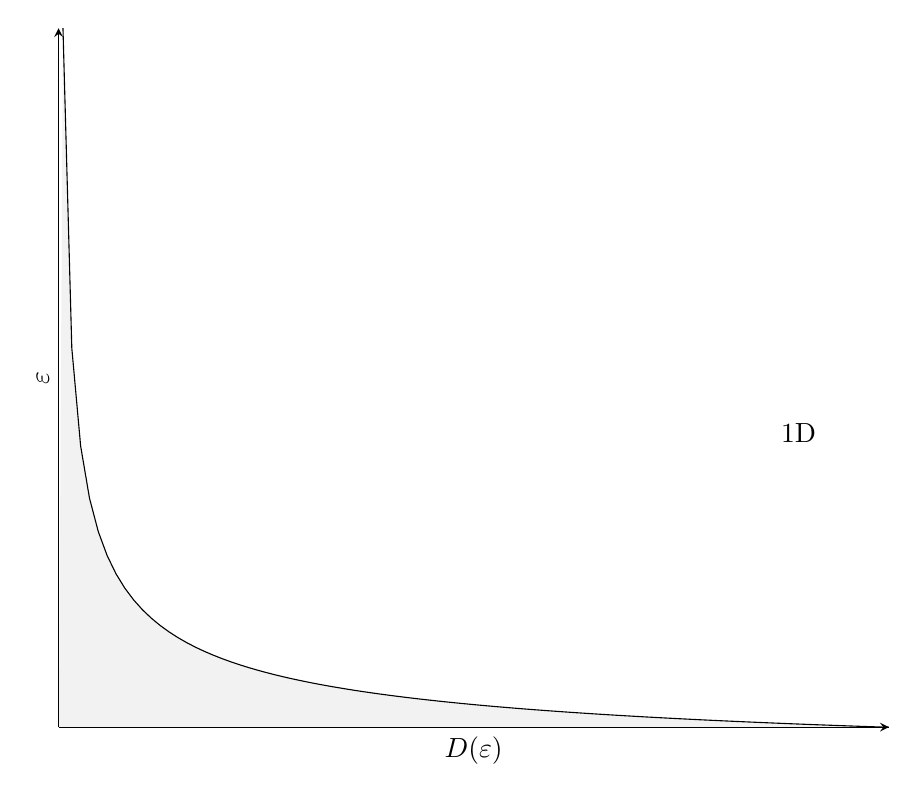
\begin{tikzpicture}
        	\begin{axis}[
        		xlabel=$D(\varepsilon)$,
        		ylabel={$\varepsilon$},
        		samples=300,
        		xmin=0,
        		xmax=pi,
        		ticks=none,
        		axis x line=bottom,
        		axis y line=left,
        		width = 1\textwidth
        	]
        	\node at (axis cs:  2.8, 3.6) {1D};
        	% use TeX as calculator:
        	\addplot+[name path=f,color=black,mark=none] {1/sqrt(x)};
        	\path[name path=axis] (axis cs:0,0) -- (axis cs:1,0);
        	\addplot [thick,color=black,fill=black,fill opacity=0.05] fill between[of=f and axis];
        	\end{axis}
        \end{tikzpicture}
    \end{minipage}\begin{minipage}{0.33\textwidth}
        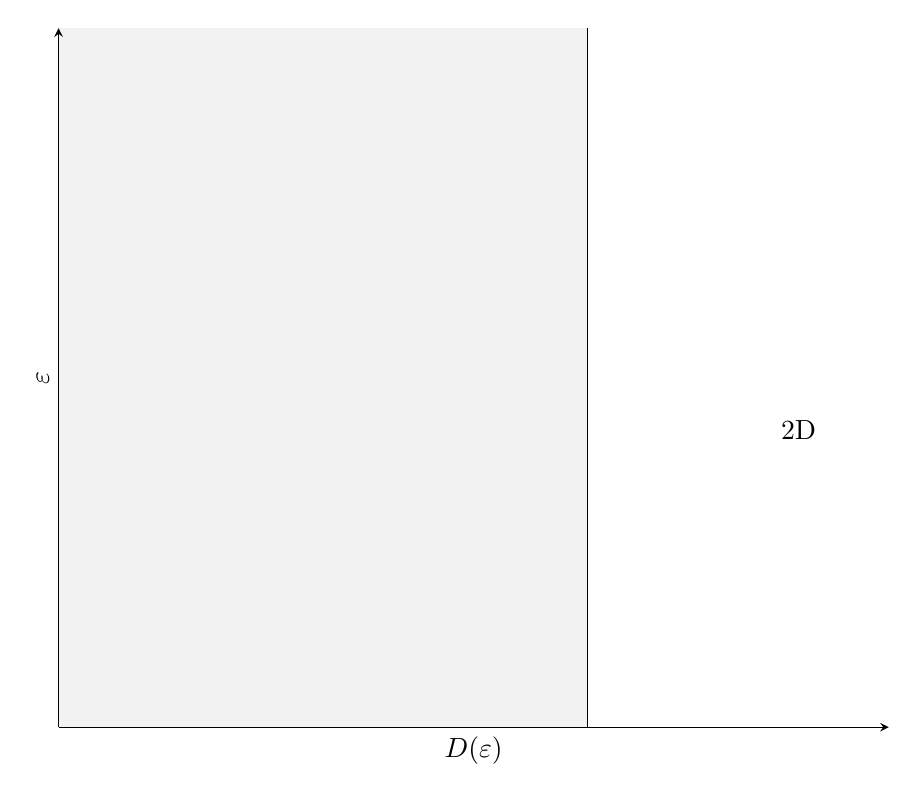
\begin{tikzpicture}
        	\begin{axis}[
        		xlabel=$D(\varepsilon)$,
        		ylabel={$\varepsilon$},
        		samples=300,
        		xmin=0,
        		xmax=pi,
        		ticks=none,
        		axis x line=bottom,
        		axis y line=left,
        		width = 1\textwidth
        	]
        	\node at (axis cs:  2.8,  0.7) {2D};
        	% use TeX as calculator:
        	\addplot +[name path=f,mark=none,color=black] coordinates {(2, -1) (2, 3)};
        	\path[name path=axis] (axis cs:0,-1) -- (axis cs:0,5);
        	\addplot [thick,color=black,fill=black,fill opacity=0.05] fill between[of=f and axis];
        	\end{axis}
        \end{tikzpicture}
    \end{minipage}\begin{minipage}{0.33\textwidth}
        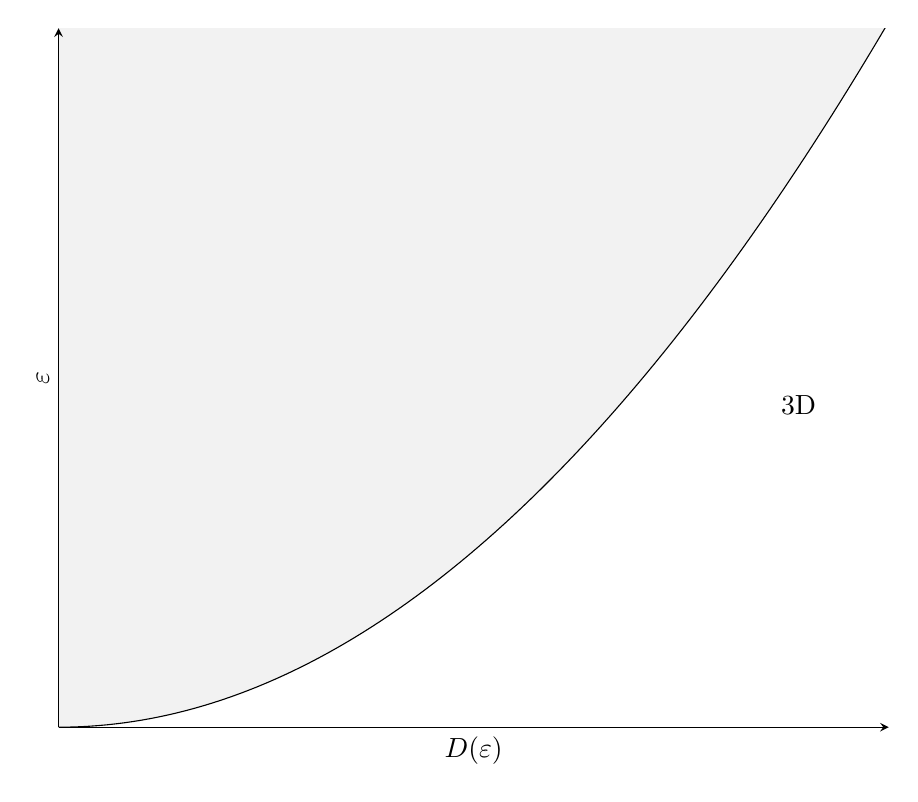
\begin{tikzpicture}
        	\begin{axis}[
        		xlabel=$D(\varepsilon)$,
        		ylabel={$\varepsilon$},
        		samples=300,
        		xmin=0,
        		xmax=pi,
        		ticks=none,
        		axis x line=bottom,
        		axis y line=left,
        		width = 1\textwidth
        	]
        	\node at (axis cs:  2.8,  4.5) {3D};
        	% use TeX as calculator:
        	\addplot+[name path=f,color=black,mark=none] {x^2};
        	\path[name path=axis] (axis cs:0,0) -- (axis cs:0,10);
        	\addplot [thick,color=black,fill=black,fill opacity=0.05] fill between[of=f and axis];
        	\end{axis}
        \end{tikzpicture}
    \end{minipage}
    \label{fig:p1f1}
    \caption{Density of states (DOS) in 1D, 2D, and 3D for the free electron gas.}
\end{figure}
\end{solution}

\subsection{Section 2; 1D chain \& dimer}
In this section we deal with three cases of a 1D chain. The simple case with one atom per unit cell, then with two atoms per unit cell, and lastly with alternating lattice spacing. All cases are schematically illustrated in figure \ref{fig:1D_Chain}.
\begin{figure}[!ht]
    \centering
    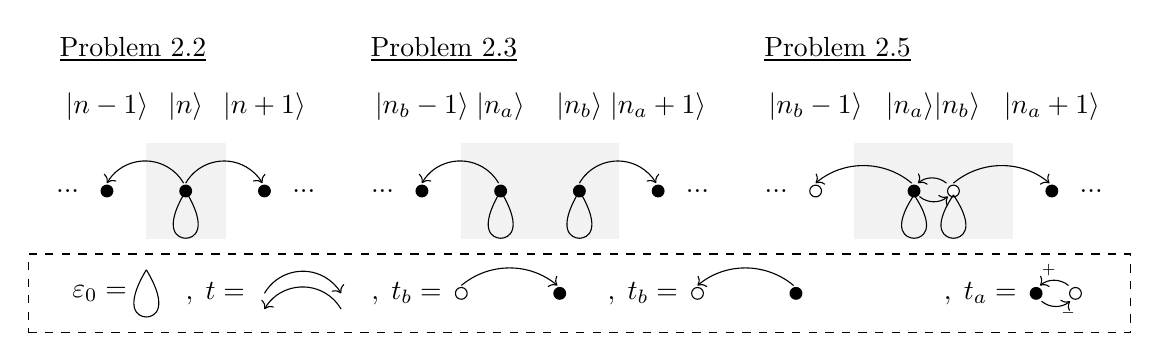
\begin{tikzpicture}[label distance = 0.7cm,
        mydot2/.style={circle, fill=white, draw, outer sep=0pt, inner sep=1.5pt},
        mydot1/.style={circle, fill=black, draw, outer sep=0pt, inner sep=1.5pt}]
        %%%%%%%%%% Label
            \node[label={[label distance = 0cm]east:{\underline{Problem 2.2}}}] at (-0.85,1.8) {};
            \node[label={[label distance = 0cm]east:{\underline{Problem 2.3}}}] at (3.1,1.8) {};
            \node[label={[label distance = 0cm]east:{\underline{Problem 2.5}}}] at (8.1,1.8) {};
        
        
        %%%%%%%%%% Legend
            \draw[dashed] (-1,-1.8) -| (13,-0.8) -| (-1,-1.8);
            
            % Epsilon
            \draw (0.5,-1) .. controls (0.2,-1.5) and (0.4,-1.6).. (0.5,-1.6)
                    (0.5,-1.6) .. controls (0.6,-1.6) and (0.8,-1.5) .. (0.5,-1);
            \node[label={[label distance = 0cm]west:{$\varepsilon_0 = $}}] at (0.5,-1.3) {};
        
            % T
            \draw [<-] (2,-1.5) arc (150:30:16pt); \draw [->] (2,-1.3) arc (150:30:16pt);
            \node[label={[label distance = 0cm]west:{$,\; t = $}}] at (2,-1.3) {};
            
            % Ta
            \draw [->] (4.5,-1.2) arc (130:50:27pt); \node[mydot2] at (4.5,-1.3) {}; \node[mydot1] at (5.75,-1.3) {};
            \node[label={[label distance = 0cm]west:{$,\; t_b = $}}] at (4.5,-1.3) {};
            
            % Tb
            \draw [<-] (7.5,-1.2) arc (130:50:27pt); \node[mydot2] at (7.5,-1.3) {}; \node[mydot1] at (8.75,-1.3) {};
            \node[label={[label distance = 0cm]west:{$,\; t_b = $}}] at (7.5,-1.3) {};
            
            % Ta - Tb
            \node[mydot1] at (11.8,-1.3) {}; \node[mydot2] at (12.3,-1.3) {};
            \draw [<-] (11.85,-1.2) arc (130:50:8pt); \draw [<-,rotate=180,shift={(-24.08,0.2)}] (11.85,1.2) arc (130:50:8pt);
            \node[label={[label distance = 0cm]west:{$,\; t_a = $}}] at (11.8,-1.3) {};
            \node[label={[label distance = 0cm]west:{\tiny{$+$}}}] at (12.3,-1) {};
            \node[label={[label distance = 0cm]west:{\tiny{$-$}}}] at (12.55,-1.55) {};
            
        
        %%%%%%%%%% problem 2.2
    	\node at (-0.5,0) {...}; \node at (2.5,0) {...};
    	\filldraw[fill=black!5!white, draw=black!5!white] (0.5,-0.6) rectangle (1.5,0.6);
    	\node[mydot1,label={above:{$\ket{n-1}$}}] (N11) at (0,0) {};
    	\node[mydot1,label={above:{$\ket{n}$}}] (N12) at (1,0) {};
    	\node[mydot1,label={above:{$\ket{n+1}$}}] (N13) at (2,0) {};
    	
        	%interaction
            \draw [<-] (0,0.1) arc (150:30:16pt); \draw [->] (1,0.1) arc (150:30:16pt);
            \draw (1,0) .. controls (0.7,-0.5) and (0.9,-0.6).. (1,-0.6)
                    (1,-0.6) .. controls (1.1,-0.6) and (1.3,-0.5) .. (1,0);
                
    	%%%%%%%%%% problem 2.3
    	\node at (3.5,0) {...}; \node at (7.5,0) {...};
    	\filldraw[fill=black!5!white, draw=black!5!white] (4.5,-0.6) rectangle (6.5,0.6);
    	\node[mydot1,label={above:{$\ket{n_b-1}$}}] (N21) at (4,0) {};
        \node[mydot1,label={above:{$\ket{n_a}$}}] (N22) at (5,0) {};
    	\node[mydot1,label={above:{$\ket{n_b}$}}] (N23) at (6,0) {};
    	\node[mydot1,label={above:{$\ket{n_a+1}$}}] (N24) at (7,0) {};

        	% interaction
        	\draw [<-] (4,0.1) arc (150:30:16pt); \draw [->] (6,0.1) arc (150:30:16pt);
            \draw (5,0) .. controls (4.7,-0.5) and (4.9,-0.6).. (5,-0.6)
                    (5,-0.6) .. controls (5.1,-0.6) and (5.3,-0.5) .. (5,0);
            \draw (6,0) .. controls (5.7,-0.5) and (5.9,-0.6).. (6,-0.6)
                    (6,-0.6) .. controls (6.1,-0.6) and (6.3,-0.5) .. (6,0);
                
    	%%%%%%%%%% problem 2.5
    	\node at (8.5,0) {...}; \node at (12.5,0) {...};
    	\filldraw[fill=black!5!white, draw=black!5!white] (9.5,-0.6) rectangle (11.5,0.6);
    	\node[mydot2,label={above:{$\ket{n_b-1}$}}] (N31) at (9,0) {};
    	\node[mydot1,label={above:{$\ket{n_a} \;$}}] (N32) at (10.25,0) {};
    	\node[mydot2,label={above:{$\; \ket{n_b}$}}] (N33) at (10.75,0) {};
    	\node[mydot1,label={above:{$\ket{n_a+1}$}}] (N34) at (12,0) {};

            % interaction
            \draw [<-] (9,0.1) arc (130:50:27pt); \draw [->] (10.75,0.1) arc (130:50:27pt);
            \draw [<-] (10.3,0.1) arc (130:50:8pt); \draw [<-,rotate=180,shift={(-20.98,-0.03)}] (10.3,0.1) arc (130:50:8pt);
            \draw (10.25,-0.05) .. controls (9.95,-0.5) and (10.15,-0.6).. (10.25,-0.6)
                    (10.25,-0.6) .. controls (10.35,-0.6) and (10.55,-0.5) .. (10.25,-0.05);
            \draw (10.75,-0.05) .. controls (10.45,-0.5) and (10.65,-0.6).. (10.75,-0.6)
                    (10.75,-0.6) .. controls (10.85,-0.6) and (11.05,-0.5) .. (10.75,-0.05);    
\end{tikzpicture}
    \caption{Schematic illustration of the orbitals, interactions, and numbering, of the 1D chains belonging to problem 2.2, 2.3, and 2.5.}
    \label{fig:1D_Chain}
\end{figure}

\begin{exercise}
show that the state 
\begin{equation}
    \ket{k} = \sum_{n = - \infty}^{\infty} e^{ikna} \ket{n}
    \label{eq:1.8}
\end{equation}
satisfies a discrete version of Bloch's theorem.
\end{exercise}

\begin{solution}
The approach is to take the inner product of the state with a projection $\bra{n+U}$, and show this is the same as $\braket{n}{k}$ up to a phase difference.
\begin{equation}
    \braket{n+U}{k} = \mel{n+U}{\sum_{n'=-\infty}^{\infty}e^{ikn'a}}{n'}
\end{equation}
This is only non-zero for $n'=n+U$, so
\begin{equation}
    \braket{n+U}{k} = \mel{n+U}{e^{ik(n+U)a}}{n+U} = e^{ik(n+U)a}\braket{n+U}{n+U} = e^{ikna}e^{ikUa}
\end{equation}
But from \eqref{eq:1.8} we have $\braket{n}{k} = e^{ikna}$, so the above reduces to
\begin{equation}
    \braket{n+U}{k} = \braket{n}{k}e^{ikUa}
\end{equation}
Thus it satisfies a discrete version of Bloch's theorem.


\end{solution}

\begin{exercise}
Calculate the band energies, $\varepsilon(k)$, for the wave vector $k$ in the first Brillouin zone, $k \in [-\frac{\pi}{a},\frac{\pi}{a}]$. Sketch the band structure and the density of states (DOS). Determine the center and width of the electronic band.
\end{exercise}
\begin{solution}
The band energies are found from
\begin{equation}
    \hat{H}\ket{k} = \varepsilon(k)\ket{k}
\end{equation}
So on applying the operator
\begin{equation}
    \hat{H}\ket{k} = \sum_n \varepsilon_0 c_n^{\dagger} c_n + t c_{n-1}^{\dagger} c_n + t c_{n+1}^{\dagger}c_n \sum_{n'} e^{ikn'a} \ket{n'}
\end{equation}
There will only be contributions from the 3 states $\ket{n'} = \ket{n} \text{ or } \ket{n \pm 1}$, so it reduces to
\begin{equation}
    \hat{H}\ket{k} = \sum_n \left[ \varepsilon_0 e^{ikna} + t e^{ik(n+1)a} + t e^{ik(n-1)a} \right] \ket{n} =  \left[ \varepsilon_0 + t e^{ika} + t e^{-ika} \right] \sum_n e^{ikna} \ket{n}
\end{equation}
According to equation \ref{eq:1.8}, and using that the complex exponentials in the square brackets can be written as 2 times cos this reduces to
\begin{equation}
   \varepsilon = \varepsilon_0 + 2 t \cos(ka) \ket{k}
   \label{eq:114}
\end{equation}

\begin{figure}
    \centering
    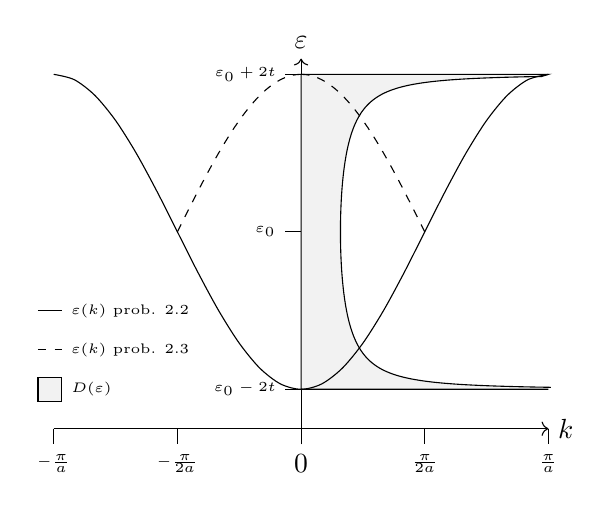
\begin{tikzpicture}
    % Axes
    \draw[->] (-pi,0) -- (pi,0) node[right] {$k$};
    \draw[->] (0,-0.2) -- (0,4.7) node[above] {$\varepsilon$};
    
    % Ticks
        %y
        \draw (0,4.5) -- (-0.2,4.5) node[left] {\tiny{$\varepsilon_0 + 2t$}};
        \draw (0,2.5) -- (-0.2,2.5) node[left] {\tiny{$\varepsilon_0$}};
        \draw (0,0.5) -- (-0.2,0.5) node[left] {\tiny{$\varepsilon_0 - 2t$}};
        
        %x
        \draw (-pi,0)   -- (-pi,-0.2)    node[below] {\tiny{$-\frac{\pi}{a}$}};
        \draw (-pi/2,0) -- (-pi/2,-0.2)  node[below] {\tiny{$-\frac{\pi}{2a}$}};
        \draw (0,0)     -- (-0,-0.2)     node[below] {$0$};
        \draw (pi/2,0)  -- (pi/2,-0.2)   node[below] {\tiny{$\frac{\pi}{2a}$}};
        \draw (pi,0)    -- (pi,-0.2)     node[below] {\tiny{$\frac{\pi}{a}$}};
    
    % Legend
    \draw (-pi-0.2,1.5) -- (-pi+0.1,1.5) node[right] {\tiny{$\varepsilon(k)$ prob. 2.2}};
    \draw[dashed] (-pi-0.2,1) -- (-pi+0.1,1) node[right] {\tiny{$\varepsilon(k)$  prob. 2.3}};
    \draw (-pi-0.2,0.5) -- (-pi+0.1,0.5) node[right] {\tiny{$D(\varepsilon)$}};
    \filldraw[fill=black!5!white] (-pi-0.2,0.35) rectangle (-pi+0.1,0.65);
    
    % DOS
    \filldraw[color=black,fill=black!5!white,smooth,samples=1000,variable=\y,domain=0.525:4.475] (0,0.5) -- (pi,0.5) plot ({(1/2)/(sqrt(1-(\y-2.5)*(\y-2.5)/4))},{\y}) --(pi,4.5) -- (0,4.5) -- (0,0.5);
    
    % Bands
    \draw[color=black,smooth,domain=-pi:pi]  plot (\x,{2.5-2*cos(\x r)});
    \draw[color=black,dashed,smooth,domain=-pi:(-pi/2)]  plot (\x+pi,{2.5-2*cos(\x r)});
    \draw[color=black,dashed,smooth,domain=(pi/2):pi]  plot (\x-pi,{2.5-2*cos(\x r)});
\end{tikzpicture}

    \caption{dispersion relation and DOS of the 1D chain in a 1 atom/unit cell (solid line) and 2 atoms/unit cell (dashed line).}
    \label{fig:1D_dispersion}
\end{figure}
    $\varepsilon(k) = \varepsilon_0 + 2 t \cos(ka)$ is sketched in figure \ref{fig:1D_dispersion}. 
    The density of states is found from isolating $k$ in $\varepsilon(k)$, and taking the derivative $D(\varepsilon) = \dv{k}{\varepsilon}$.
    \begin{equation}
        k(\varepsilon) = \frac{1}{a} \arccos\left(\frac{\varepsilon -\varepsilon_0}{2t} \right) \Rightarrow D(\varepsilon) = -\frac{1}{2ta} \frac{1}{\sqrt{1-\left(\frac{\epsilon-\epsilon_0}{2t} \right)^2}}
    \end{equation}
    The bandwidth is $4t$
\end{solution}

\begin{exercise}
Argue that the wave functions of the dimerized chain must have the form
\begin{equation}
    \ket{ks} = \sum_{n=-\infty}^{\infty} e^{ik(a+b)n} \left[ c_{as} \ket{n_a} + c_{bs} \ket{n_b} \right]
\end{equation}
\end{exercise}

\begin{solution}
It makes sense that the solution is found as a superposition of the states of the individual a and b states. No matter what these can serve as a basis for the solution.
$s=1,2$ as there will be two energy bands in this 2-state system.
\end{solution}

\begin{exercise}
Calculate the wave functions $\ket{sk}$ and band energies $\varepsilon_s(k)$. Sketch the
band structure and DOS of the dimerized chain, and determine the size of
the band gap, $E_{gap}$.
\end{exercise}

\begin{solution}
The system can be seen in the right most illustration in figure \ref{fig:1D_Chain}.
The Hamiltonian consists of 2 terms, that correspond to no jumping. Two terms of jumping within the unit cell, and two terms of jumping out of the cell, as illustrated in figure \ref{fig:1D_Chain}. Thus it is
\begin{equation}
    \hat{H} = \varepsilon_0 c_{na}^{\dagger}c_{na} + \varepsilon_0 c_{nb}^{\dagger}c_{nb} + t_a (c_{na}^{\dagger} c_{nb} + c_{nb}^{\dagger} c_{na} ) + t_b (  c_{(n-1)b}^{\dagger} c_{na} + c_{(n+1)a}^{\dagger} c_{nb})
\end{equation}
Where $t_a$ is the energy associated with jumping within the unit cell, and $t_b$ is associated with jumping out of the unit cell. \\
This system is put in matrix form in the $\ket{a}$ and $\ket{b}$ basis, and the eigenvalues and eigenfunctions will be found from diagonalising.
\begin{equation}
    \hat{H}_{ab} =
    \begin{bmatrix}
    \mel{a}{H}{a} & \mel{a}{H}{b} \\
    \mel{b}{H}{a} & \mel{b}{H}{b}
    \end{bmatrix}
\end{equation}
The diagonal terms only get contributions from the non-hopping elements. The off diagonal terms get contributions from hopping terms that go outside the unit cell, in this case a phase factor is multiplied on, applying Bloch's theorem.
\begin{equation}
    \hat{H}_{ab} =
    \begin{bmatrix}
    \varepsilon_0 & t_a + t_b e^{-ik(a+b)} \\
    t_a + t_b e^{ik(a+b)} & \varepsilon_0
    \end{bmatrix}
\end{equation}
Thus the energies are
\begin{equation}
\begin{split}
    (\varepsilon_0 - \lambda)^2 - (t_a + t_b e^{-ik(a+b)})(t_b + t_a e^{ik(a+b)}) = 0 \\ = (\varepsilon_0 - \lambda)^2 - (t_a^2 + t_b^2 + t_a t_b (e^{ik(a+b)} + e^{-ik(a+b)})) \\ = (\varepsilon_0 - \lambda)^2 - t_a^2 - t_b^2 - 2 t_a t_b \cos(k(a+b)) \\
    \Rightarrow \lambda =  \varepsilon_0 \mp \sqrt{ t_a^2 + t_b^2 + 2 t_a t_b \cos(k(a+b))}
\end{split}
\end{equation}



\begin{figure}
    \centering
    \begin{tikzpicture}
    % Axes
    \draw[->] (-pi,0) -- (pi,0) node[right] {$k$};
    \draw[->] (0,-0.2) -- (0,4.7) node[above] {$\varepsilon$};
    
    % Ticks
        %y
        \draw (-0.3,4.5)  (-0.5,4.5) node[left] {\tiny{$\varepsilon_0 + ta + tb$}};
        \draw (0,2.5) -- (-0.2,2.5) node[left] {\tiny{$\varepsilon_0$}};
        \draw (-0.3,0.5)  (-0.5,0.5) node[left] {\tiny{$\varepsilon_0 - ta - tb$}};
        
        %x
        \draw (-pi,0)   -- (-pi,-0.2)    node[below] {\tiny{$-\frac{\pi}{a}$}};
        \draw (-pi/2,0) -- (-pi/2,-0.2)  node[below] {\tiny{$-\frac{\pi}{2a}$}};
        \draw (0,0)     -- (-0,-0.2)     node[below] {$0$};
        \draw (pi/2,0)  -- (pi/2,-0.2)   node[below] {\tiny{$\frac{\pi}{2a}$}};
        \draw (pi,0)    -- (pi,-0.2)     node[below] {\tiny{$\frac{\pi}{a}$}};
    
    % Legend
    %\draw (-pi-0.2,1) -- (-pi+0.1,1) node[right] {\tiny{$\varepsilon(k)$}};
    %\draw (-pi-0.2,0.5) -- (-pi+0.1,0.5) node[right] %{\tiny{$D(\varepsilon)$}};
    %\filldraw[fill=black!5!white] (-pi-0.2,0.35) rectangle %(-pi+0.1,0.65);
    
    % DOS
    
    % Bands, ta=2/3, tb = 4/3, epsilon=2.5
    \draw[color=black,smooth,domain=-pi:pi]  plot (\x,{2.5-sqrt(4/9+16/9+16/9*cos(\x r))});
    \draw[color=black,smooth,domain=-pi:pi]  plot (\x,{2.5+sqrt(4/9+16/9+16/9*cos(\x r))});
\end{tikzpicture}

    \caption{dispersion relation and DOS of the 1D dimerised chain. Recalling that the short and long latice spacing, $a'$ and $b$ respectively, satisfy $a'+b = 2a$ where $a$ is the latice spacing of the non-dimerized chain.}
    \label{fig:1D_Dimer}
\end{figure}
It is seen that the energy of the lower band is lower in the dimerised case. This would imply that dimerisation is energetically favourable. However, the Coulomb energy is not taken into account in this model, and therefor there will be a competing term trying to create equal spacing. 
\end{solution}


\subsection{Section 3; Intuition on band structure}
\begin{exercise}
Sketch the band structure and the density of states (DOS) of: (A) an alkali
metal, (B) a noble metal, early (C) and late (D) transition metal, direct (E) and indirect (F) semi-conductor, and semi-metal (G) and graphene (H). 
\end{exercise}

\begin{solution}
TABLE of characteristics. \\
FIGURES comming up.
\end{solution}


\newpage \section{Week 2: Linear response}
\textbf{Remarks about this exercise set:}
We are studying how physical quantities change when subject to weak perturbations. The fact that we're studying weak perturbations allows us to base our analysis on time-dependent perturbation theory to first order. In its essence, this exercise allow us to describe how quantities change to due weak perturbations and of particular interest we looked at how the electron-density changes as a consequence of an applied (scalar) potential.

\textit{Comments on the interaction picture (IP).} Typically smart when the Hamiltonian can be split up into a simple part which shall be denoted $\HO$ and a remainder $V$. In the IP, time-evolution of the operators are taken to be in the Heisenberg picture wrt. $\HO$, i.e., for a given operator of $\hat{A}_{H_{0}}$ we have that $\hat{A}_{H_{0}}\qty(t) = e^{i\HO t} \hat{A}qty(t)e^{-i\HO t_0}$. The remaining time-dependence due to $\hat{V}$ is \textit{carried} through the state-vector with help from the IP time-evolution operator $\hat{U}_I\qty(t, t_0)$ given as Eq. (1) in the exercise-sheet. Additionally, we also utilise the IP given that the Hamiltonian of a system is time-dependent. 

\subsection{Section 2; Linear response of time-independent variables}
\begin{exercise}
Show that the change in the (time-independent) observable $\hat{A}$ at time $t = 0$ to linear order in $\hat{V}$ is:
\begin{equation}
    \delta A(t=0) = -i\int_{t_0}^{\infty}\theta(-t')\expval{\comm{\hat{A}_{\hat{H}_0}(0)}{\hat{V}_{\hat{H}_0}}(t')}{0}\mathrm{d}t
\end{equation}
\end{exercise}

\begin{solution}
The change in any observable, due to a perturbation is given by
\begin{equation}
    \delta A(t=0) = \mel{0}{\hat{U}(0)^{\dagger} \hat{A} \hat{U}(0)}{0} - \mel{0}{\hat{A}}{0}
    \label{eq:2.2}
\end{equation}

The operator $\hat{U}$ is given in equation (3) in the problem handout can be Taylor expanded as
\begin{equation}
    \hat{U} \approx \hat{T}(1-i \int_{t_0}^0 \hat{V}_{\hat{H}_0}(t') \text{d}t')\mathrm{e}^{i\hat{H}_0t_0}
    \label{eq:2.3}
\end{equation}
$\hat{A}$ is time independent, so upon inserting equation \ref{eq:2.3} in \ref{eq:2.2}, the time ordering operator is unnecessary. Furthermore, the potential must be real, so that  $V_{\hat{H}_0}^{\dagger} = V_{\hat{H}_0}$. Thus:
{\small \begin{equation}
\begin{split}
        \delta A(t=0) = \mel{0}{\mathrm{e}^{-i\hat{H}_0t_0}\left( 1+i \int_{t_0}^0 \hat{V}_{\hat{H}_0}(t') \text{d}t' \right) \hat{A} \left( 1-i \int_{t_0}^0 \hat{V}_{\hat{H}_0}(t') \text{d}t'\right)\mathrm{e}^{i\hat{H}_0t_0}}{0} - \mel{0}{\hat{A}}{0} \\
        = \mel{0}{\hat{A}}{0} + \mel{0}{i \int_{t_0}^0 \hat{V}_{\hat{H}_0}(t') \text{d}t' \hat{A}}{0} - \mel{0}{\hat{A} i \int_{t_0}^0 \hat{V}_{\hat{H}_0}(t') \text{d}t'}{0} - \mel{0}{\mathcal{O}(\hat{V}_{\hat{H}_0}^2)}{0} - \mel{0}{\hat{A}}{0}
\end{split}
\end{equation}}
Where the operators $\mathrm{e}^{\pm i \hat{H}_0t_0}$ acting to either right or left simply gives $\mathrm{e}^{\pm i E_0 t_0}$ hence it will cancel. \textbf{NB!} the sign of the complex exponential function does not change when acting on the bra instead of the ket!
As $\hat{A}$ is time independent we have
\begin{equation}
    \hat{A}_{\hat{H}_0} = e^{-i\hat{H}_0t} \hat{A} e^{i \hat{H}_0 t} = \hat{A}
\end{equation}
Furthermore, it must commute with the time integral. The states $\ket{0}$ are time independent as well, so in fact the integral can be moved outside of the inner products, thus:
\begin{equation}
\begin{split}
        \delta A(t=0) = i\int_{t_0}^0 \left(\mel{0}{\hat{V}_{\hat{H}_0}(t') \hat{A}_{\hat{H}_0}(0)}{0} - \mel{0}{\hat{A}_{\hat{H}_0}(0) \hat{V}_{\hat{H}_0}(t')}{0}\right) \text{d}t' \\ = - i \int_{t_0}^0 \mel{0}{\comm{\hat{A}_{\hat{H}_0}(0)}{ \hat{V}_{\hat{H}_0}(t')}}{0} \text{d}t' = - i \int_{t_0}^{\infty} \theta(-t') \mel{0}{\comm{\hat{A}_{\hat{H}_0}(0)}{ \hat{V}_{\hat{H}_0}(t')}}{0} \text{d}t'
        \label{eq:Sol:21}
\end{split}
\end{equation}
This we often denote by $C_{AV}^{r}$ as given below:
\begin{equation}
    \delta A(t=0) = \int_{t_0}^{\infty}C_{AV}^{r}(t')\mathrm{d}t'
\end{equation}
\textbf{Note: A is time independent everything else is completely general}
\end{solution}

\subsection{Section 2; Harmonic time-dependence (the Kubo formula)}

\begin{exercise}
Now assume that the perturbation has a harmonic time-dependence $\hat{V} (t) = \mathrm{e}^{-i(\omega +i\eta)t}\hat{V}$ and is turned on adiabatically (very slowly) at time $t_0 = -\infty$, (through $\eta$). Use the identity $\hat{I} = \sum_{s} \ket{s}\bra{s}$ to show that in this case the change in the observable $A$ becomes:
\begin{equation}
    \delta A(\omega + i\eta) = \sum_{s} \dfrac{\mel{0}{\hat{A}}{s}\mel{s}{\hat{V}}{0}}{\omega - \omega_{s0} + i\eta} - \dfrac{\mel{0}{\hat{V}}{s}\mel{s}{\hat{A}}{0}}{\omega + \omega_{s0} + i\eta} 
\end{equation}
where $\omega_{s0} = E_s - E_0$ is the difference between the groundstate and s'th excited state energy of $\hat{H}_0$.
\end{exercise}
\begin{solution}
In order to use Kabo's formula we need to transform $\hat{V}$ into the basis of the unperturbed Hamiltonian, i.e. $\hat{V}_{\hat{H}_0}(t) = \mathrm{e}^{i\hat{H}_0t}\mathrm{e}^{-i(\omega + i\eta)}\hat{V}\mathrm{e}^{-i\hat{H}_0t}$. We still have that $\hat{A}_{\hat{H}_0} = \hat{A}$ due to time-independence.
Inserting into Kabo's forumla we get:
\begin{equation}
    \delta A(\omega + i\eta) = \int_{-\infty}^{0}-i \mel{0}{\comm{\hat{A}_{\hat{H}_0}}{\hat{V}_{\hat{H}_0}(t')}}{0}\mathrm{d}t'
\end{equation}
Focusing only on the first term of the commutator and using the identity $\hat{I} = \sum_{s} \ket{s}\bra{s}$, as well as the fact that the sum over $s$ commutes with the integral to obtain:
\begin{equation}\label{eq:p2q10}
    \sum_{s}\int_{-\infty}^{0}-i \mel{0}{\hat{A}_{\hat{H}_0} \ket{s}\bra{s}\mathrm{e}^{i\hat{H}_0t}\mathrm{e}^{-i(\omega + i\eta)}\hat{V}\mathrm{e}^{-i\hat{H}_0t}}{0}\mathrm{d}t'
\end{equation}
The effect of the operators is $\mathrm{e}^{i\hat{H}_0t}\ket{s} = \mathrm{e}^{i\omega_st}\ket{s}$, (and $\bra{s}\mathrm{e}^{i\hat{H}_0t} = \bra{s}\mathrm{e}^{i\omega_st}$), this is obtained through the series expansion of $\mathrm{e}^{i\hat{H}_0t}$ acting on the state. Hence \eqref{eq:p2q10} can be stated in a more compact form, by taking the exponentials outside, as they are just constants, and substituting back $\hat{A}_{\hat{H}_0} = \hat{A}$:
\begin{equation}
    \sum_{s}\int_{-\infty}^{0}-i\mathrm{e}^{-i(\omega + i\eta -\omega_0 + \omega_s)t} \mel{0}{\hat{A}} {s}\mel{s}{\hat{V}}{0}\mathrm{d}t'
\end{equation}
Noting here that the other part of the commutator is obtained by letting the $\pm \hat{H}_0$ operator act on the opposite states i.e. we obtain $+\omega_0 - \omega_s$ in the exponent instead. As both $\hat{A}$ and $\hat{V}$ is independent of time they commute with the integral which is trivially integrated to get:
\begin{equation}
    \sum_{s}\mel{0}{\hat{A}} {s}\mel{s}{\hat{V}}{0}\left[\dfrac{-i\mathrm{e}^{-i(\omega + i\eta -\omega_0 + \omega_s)}}{-i(\omega -\omega_{s0} + i\eta)t}\right]_{-\infty}^{0} = \sum_{s}\dfrac{\mel{0}{\hat{A}} {s}\mel{s}{\hat{V}}{0}}{\omega -\omega_{s0} + i\eta}
\end{equation}
Repeating the same operation for the other part of the commutator shifts the operators $\hat{A}$ and $\hat{V}$ as well as the sign on $\omega_{s0}$ hence we obtain the solution:
\begin{equation}
    \delta A(\omega + i\eta) = \sum_{s} \dfrac{\mel{0}{\hat{A}}{s}\mel{s}{\hat{V}}{0}}{\omega - \omega_{s0} + i\eta} - \dfrac{\mel{0}{\hat{V}}{s}\mel{s}{\hat{A}}{0}}{\omega + \omega_{s0} + i\eta} 
    \label{eq:Kubo}
\end{equation}
The result is complex because we introduced the harmonic potential through the complex exponential. Consequently we must take the real part to obtain a pertubation of the form $\cos(\omega t)\hat{V}$ or imaginary part for the form $\sin(\omega t)\hat{V}$. As $\eta$ was introduced to turn on the harmonic pertubation adiabatically we must take the limit $\lim_{\eta\rightarrow0}\mathrm{Re,Im}[\delta A(\omega+i\eta)]$ to obtain the real solution. \textbf{NB!} the real and imaginary operator does not commute with the limit.
\end{solution}


\subsection{Section 3; Kramers-Kronig relations}
\begin{exercise}
The derivation of the Kramers-Kronig relations.
\end{exercise}
\begin{solution}
Equation 9 in the problem handout can in the notation $z \rightarrow \omega$, can be written as
\begin{equation}
    F(\omega) = \int_{0}^{\infty} e^{i \omega t}F(t) \text{d}t
\end{equation}
 This integral is finite as long as $F(t)$ does not grow exponentially or faster.
 Furthermore it has no poles, which means that the function
 \begin{equation}
     \frac{F(\omega')}{\omega - \omega' + i \eta}
 \end{equation}
 only has a single pole, slightly below the real axis. Integrating the above function around a contour that runs along the real axis, and follows a halfcircle with a radius going to infinity along the upper half of the complex plane must thus equal 0. \\
 Furthermore the function goes to zero when $\abs{\omega'}$ goes to infinity, so the integral along the upper half plane is also equal to zero. This means that an integral along the entire real axis must also equal zero, so
 \begin{equation}
     \int_{-\infty}^{\infty} \frac{F(\omega')}{\omega - \omega' + i \eta} \text{d} \omega' = 0
 \end{equation}
 Using the identity given by equation 13 in the problem handout, with $x=\omega-\omega'$, we obtain
 \begin{equation}
     \int_{-\infty}^{\infty} F(\omega') \left(\frac{\mathcal{P}}{\omega-\omega'} - i \pi \delta(\omega-\omega') \right)\text{d}\omega' = \mathcal{P}\int_{-\infty}^{\infty} \frac{F(\omega')}{\omega-\omega'} \text{d} \omega'- i \pi F(\omega)= 0
 \end{equation}
 For the above equation to be true both the real and imaginary parts must equal zero. Taking the real part of the above equation and using $\text{Re}(i f(x)) = -\text{Im}(f(x))$ yields
 \begin{equation}
     \mathcal{P} \int_{-\infty}^{\infty} \frac{\text{Re}(F(\omega'))}{\omega'-\omega} \text{d} \omega' + \pi \text{Im}(F(\omega)) = 0 \Leftrightarrow \text{Im}(F(\omega)) = -\frac{\mathcal{P}}{\pi} \int_{-\infty}^{\infty} \frac{\text{Re}(F(\omega'))}{\omega'-\omega} \text{d} \omega'
 \end{equation}
 Using equation (15) in the problem handout the above integral can be split in a sum of two integrals from 0 to infinity, where the second integral has $\omega \rightarrow - \omega$
 \begin{equation}
     \text{Im}(F(\omega)) = -\frac{\mathcal{P}}{\pi} \int_{0}^{\infty} \frac{\text{Re}(F(\omega'))}{\omega'-\omega} + \frac{\text{Re}(F(\omega'))}{\omega'+\omega} \text{d} \omega' = -\frac{\mathcal{P}}{\pi} \int_{0}^{\infty} \frac{2 \omega' \text{Re}( F(\omega'))}{\omega'^2-\omega^2} \text{d} \omega'
 \end{equation}
 
 
 
 
 Similarly for the imaginary part, using $\text{Im}(i f(x)) = +\text{Re}(f(x))$
 \begin{equation}
     \mathcal{P} \int_{-\infty}^{\infty} \frac{\text{Im}(F(\omega'))}{\omega'-\omega} \text{d} \omega' - \pi \text{Re}(F(\omega)) = 0 \Leftrightarrow \text{Re}(F(\omega)) = \frac{\mathcal{P}}{\pi} \int_{-\infty}^{\infty} \frac{\text{Im}(F(\omega'))}{\omega'-\omega} \text{d} \omega'
 \end{equation}
 Using equation 14 in the problem handout this integral also be split up in two terms, again with $\omega \rightarrow - \omega$ in the second term.
 \begin{equation}
     \text{Re}(F(\omega)) = \frac{\mathcal{P}}{\pi} \int_{0}^{\infty} \frac{\text{Im}(F(\omega'))}{\omega'-\omega} - \frac{\text{Im}(F(\omega'))}{\omega'+\omega}\text{d} \omega' =\frac{\mathcal{P}}{\pi} \int_{0}^{\infty} \frac{2 \omega \text{Im}(F(\omega'))}{\omega'-\omega} \text{d} \omega'
 \end{equation}
 
 \textbf{Note:} The Kramer-Kronig relations thereby couple the imaginary part of the dielectric function to the real part. The imaginary part is related to absorption in a medium, whereas the real part is usually related to dispersion. Thereby different optical properties are seen to be coupled to each other.
\end{solution}



\newpage
\subsection{Section 4; Density-density response}
\begin{exercise}
We now specialize to the case: $\hat{A}= \hat{n}(r)$ and $\hat{V} = \int V(r)\hat{n}(r)\mathrm{d}r$. In this case the Kubo formula gives the change in the electron density at a point $r$ when the system is subject to a potential of the form $V(r)$. Again we assume a harmonic time dependence of the applied potential which is switched on adiabatically at $t_0 = -\infty$. Show that in this case
\begin{equation}
    \delta n(r,\omega) = \int \chi(r,r',\omega) V(r')\mathrm{d}r
\end{equation}
where the density-density response function is given by
\begin{equation}
    \chi(r,r',\omega) = \sum_{i,j} \dfrac{\mel{0}{\hat{n}(r)}{s}\mel{s}{\hat{n}(r')}{0}}{\omega - \omega_{s0} + i\eta} - \dfrac{\mel{0}{\hat{n}(r')}{s}\mel{s}{\hat{n}(r)}{0}}{\omega + \omega_{s0} + i\eta}
\end{equation}
\vspace{-0.55cm}
\end{exercise}


\begin{solution}
Plugging the form of the observable and potential into equation \ref{eq:Kubo} yields
\begin{equation}
    \delta n(r,\omega) = \sum_{s} \dfrac{\mel{0}{\hat{n}(r)}{s}\mel{s}{\int V(r')\hat{n}(r')\text{d}r' }{0}}{\omega - \omega_{s0} + i\eta} - \dfrac{\mel{0}{\int V(r')\hat{n}(r')\text{d}r' }{s}\mel{s}{\hat{n}(r)}{0}}{\omega + \omega_{s0} + i\eta} 
\end{equation}
The inner product and the integral commute as they are over different variables. Thus it follows directly that
\begin{equation}
\begin{split}
        \delta n(r,\omega) = &\int V(r') \sum_{s} \dfrac{\mel{0}{\hat{n}(r)}{s}\mel{s}{\hat{n}(r') }{0}}{\omega - \omega_{s0} + i\eta} - \dfrac{\mel{0}{\hat{n}(r') }{s}\mel{s}{\hat{n}(r)}{0}}{\omega + \omega_{s0} + i\eta} \text{d}r' \\
        = & \int \chi(r,r',\omega) V(r') \text{d}r'
\end{split}
\label{eq:densitydensity}
\end{equation}


\end{solution}





\subsection{Section 6; Non-interacting density-density response}
\begin{exercise}
We now consider non-interacting electrons. In this case the eigenstates $\ket{s}$ are simply Slater determinants build from the single-particle eigenstates fulfilling $\hat{H}_0\ket{\phi_i} = \varepsilon_i\ket{\phi_i}$. Show that the non-interacting density response function takes the form
\begin{equation}
    \chi^{0}(r,r',\omega) = \sum_{i,j} (f_i-f_j)\dfrac{\phi^{*}_i(r)\phi_j(r)\phi_i(r')\phi^{*}_j(r')}{\omega - (\varepsilon_j - \varepsilon_i) + i\eta}
\end{equation}
where $f_i = \theta(\varepsilon_F-\varepsilon_i)$ is the occupation number of orbital i.
\end{exercise}

\begin{solution}
We start by evaluating the inner products, using the density operator on second quantised form $\hat{n}(r) = \sum_{ij} \phi_i^*(r)\phi_j(r)\hat{c}_i^{\dagger}\hat{c}_j$.
\begin{equation}
    \mel{0}{\hat{n}(r)}{s} = \sum_{ij}\phi_i^*(r)\phi_j(r) \mel{0}{\hat{c}_i^{\dagger} \hat{c}_j}{s} =  \sum_{ij}\phi_i^*(r)\phi_j(r) f_i(1-f_j) \delta_{s0_j^i}
\end{equation}
Where the index in the delta function denotes the i'th orbital in the groundstate (0), and the j'th orbital in the s state, and
$f$ denotes the probability of finding an electron in the state, given by the Fermi-Dirac distribution. \\
Similarly
\begin{equation}
    \mel{s}{\hat{n}(r')}{0} = \sum_{kl}\phi_k^*(r)\phi_l(r) \mel{s}{\hat{c}_k^{\dagger} \hat{c}_l}{0} = \sum_{kl} \phi_k^*(r') \phi_l(r') f_l(1-f_k) \delta_{s0_k^l}
\end{equation}
So that the product of the two is
\begin{equation}
\begin{split}
        & \mel{0}{\hat{n}(r)}{s}\mel{s}{\hat{n}(r')}{0} \\
        = & \sum_{ij}\phi_i^*(r)\phi_j(r) f_i(1-f_j) \delta_{s0_j^i} \sum_{kl} \phi_k^*(r') \phi_l(r') f_l(1-f_k) \delta_{s0_k^l}
\end{split}
\end{equation}
The delta functions cancel each other unless $i=l$ and $j=k$, so it reduces to one sum
\begin{equation}
    \sum_{ij} \phi_i^*(r)\phi_j(r) f_i^2(1-f_j)^2 \delta_{s0_j^i} \phi_j^*(r') \phi_i(r') 
\end{equation}
We are assuming so low temperatures that the Fermi-Dirac distribution is a step function, so that the above gives
\begin{equation}
        \sum_{ij} \phi_i^*(r)\phi_j(r) f_i(1-f_j) \delta_{s0_j^i} \phi_j^*(r') \phi_i(r') 
\end{equation}
Now we can write up the full equation (20) from the problem handout
\begin{equation}
    \sum_s \frac{\sum_{ij} \phi_i^*(r)\phi_j(r) f_i(1-f_j) \delta_{s0_j^i} \phi_j^*(r') \phi_i(r') }{\omega - \omega_{s0} + i \eta} - \frac{\sum_{ij} \phi_i^*(r')\phi_j(r') f_i(1-f_j) \delta_{s0_j^i} \phi_j^*(r) \phi_i(r) }{\omega + \omega_{s0} + i \eta}
\end{equation}
The s-sum only gives a contribution from exactly the state s that has the correct orbital, thereby cancelling the delta-functions.
\begin{equation}
    \frac{\sum_{ij} \phi_i^*(r)\phi_j^*(r') f_i(1-f_j)  \phi_j(r) \phi_i(r') }{\omega - \omega_{ji} + i \eta} - \frac{\sum_{ij} \phi_i^*(r')\phi_j^*(r) f_i(1-f_j)  \phi_j(r') \phi_i(r) }{\omega + \omega_{ji} + i \eta}
\end{equation}
The index is shifted in the second term as $j \leftrightarrow i$, then using $\omega_{ij} = - \omega_{ji}$, as well as $f_jf_i = 0$, we obtain
\begin{equation}
\begin{split}
       &\sum_{ij} \frac{ \phi_i^*(r)\phi_j^*(r')  \phi_j(r) \phi_i(r') }{\omega - \omega_{ji} + i \eta}(f_i(1-f_j) - f_j(1-f_i)) \\
       = &\sum_{ij} (f_i-f_j)\frac{ \phi_i^*(r)\phi_j^*(r')   \phi_j(r) \phi_i(r') }{\omega - \omega_{ji} + i \eta}
\end{split}
\label{eq:234}
\end{equation}
\end{solution}

\subsection{Section 7; Fourier properties of periodic systems}
\begin{exercise}
Show that any function that fulfills $f(r, r_0) = f(r +R, r_0 +R)$, where $R$ is a lattice vector, is block diagonal in reciprocal space, i.e. $f(G + q;G' + q') = f(G + q,G' + q)\delta_{qq'}$ . We denote $f(G + q,G' + q) = fGG'(q)$.
\end{exercise}
\begin{solution}
The approach is to write up $f(G+q,G'+q')$ using both $f(r,r')$ and $f(r+R,r'+R)$, and then figure out, what must be true for $q$ and $q'$.
\begin{align}
    f(Q,Q') &= \int\int \mathrm{e}^{iQr}f(r,r')\mathrm{e}^{-iQ'r'}\mathrm{d}r\mathrm{d}r' \\
    f(G+q,G'+q') &= \int\int \mathrm{e}^{i(G+q)r}f(r,r')\mathrm{e}^{-i(G'+q')r'}\mathrm{d}r\mathrm{d}r'
    \label{eq:236}
\end{align}
Now using $f(r+R,r'+R)$
\begin{align}
    f(G+q,G'+q') &= \int \int \mathrm{e}^{i(G+q)(R+r)} f(r+R,r'+R) \mathrm{e}^{-i(G'+q')(R+r')} \mathrm{d}r\mathrm{d}r'\\
    &=\int \int \mathrm{e}^{i(G+q)r} f(r+R,r'+R) \mathrm{e}^{-i(G'+q')r'}\mathrm{e}^{(q-q')R} \mathrm{d}r\mathrm{d}r'
    \label{eq:238}
\end{align}
Where we have used $\mathrm{e}^{iGR} = \mathrm{e}^{i2\pi n} \; ; \; n \in \mathbb{Z}$, so $\mathrm{e}^{iGR} = 1$.
If $f(r,r')$ and $f(r+R,r'+R)$ are equivalent we must also have that \eqref{eq:236} and \eqref{eq:238} are the same. For this to be true we get that
\begin{equation}
    (q-q')R = 2 \pi n \; , \; n \in \mathbb{Z}
\end{equation}
But $q$ and $q'$ are both smaller than a reciprocal lattice vector G, as they are in the first Brillouin zone, thus $\abs{(q-q')R} < 2 \pi$, therefore we must have $q=q'$, as $qR \in ]-\pi;\pi[$.
\end{solution}

\subsection{Section 7; Non-interacting density response of periodic systems}
\begin{exercise}
For a periodic system the eigenstates can be labelled $\ket{\phi_{nk}}$ where $n$ is a band index and $k$ is a wave vector in the first BZ. Show that in this case the non-interacting density response function takes the form
{\small \begin{equation}
    \chi_{G,G'}^{0}(q,\omega) = \sum_{nm}\sum_{k}(f_{nk}-f_{m(k+q)})\dfrac{\mel{\phi_{nk}}{\mathrm{e}^{i(G+q)r}}{\phi_{m(k+q)}}\mel{\phi_{m(k+q)}}{\mathrm{e}^{-i(G'+q)r}}{\phi_{nk}}}{\omega - (\varepsilon_{m(k+q)}-\varepsilon_{nk}) + i\eta}
\end{equation}}
\end{exercise}

\begin{solution}
As we are in a periodic structure, we can know the wavefunctions can be indexed by a band-number and the wavevectors k, thus we let $i \rightarrow nk$, $j \rightarrow mk'$

{\small
\begin{equation}
    \chi_{G,G'}^{0}(q,\omega) = \int \int \mathrm{e}^{i(G+q)r} \sum_{nk}\sum_{mk'}(f_{nk}-f_{mk'})\dfrac{\phi_{nk}^{*}(r)\phi_{mk'}(r)\phi_{nk}(r')\phi_{mk'}^{*}(r')}{\omega - (\varepsilon_{mk'}-\varepsilon_{nk})+i\eta}\mathrm{e}^{-i(G'+q)r'}\mathrm{d}r\mathrm{d}r'
\end{equation}}
Grouping terms in $r$ and $r'$ this can be written as two inner products
\begin{equation}
    \chi_{G,G'}^{0}(q,\omega) = \sum_{nk} \sum_{mk'} (f_{nk}-f_{mk'}) \frac{\mel{\phi_{nk}}{e^{i(G+q)r}}{\phi_{mk'}}\mel{\phi_{mk'}}{e^{-i(G'+q)r'}}{\phi_{nk}}}{\omega - (\varepsilon_{mk'}-\varepsilon_{nk})+i\eta}
\end{equation}
We now focus on only one inner product, namely the second (for no good reason), so that
\begin{align}
    \mel{\phi_{mk'}}{e^{-i(G+q)r}}{\phi_{nk}} &= \int \phi_{mk'}^{*}(r) \mathrm{e}^{-i(G+q)r}\phi_{nk}(r) \mathrm{d}r\\
    & =\int u_{mk'}^{*}\mathrm{e}^{-ik'r} \mathrm{e}^{-i(G+q)r}\mathrm{e}^{ikr}u_{nk} \mathrm{d}r \label{eq:244}
\end{align}
Above we have used that it is a periodic system, so that the wave function can be written as a product of a Bloch wave and a plane wave. 
This integral is the sum of identical integrals for all lattice vectors $R$, all given by  the integral in the first Brillouin zone. Hence we may formulate \eqref{eq:244} as the sum over all $R$ by substituting $r \rightarrow r + R$ and integrating over the first Brillouin zone.
\begin{equation}
    \mel{\phi_{mk'}}{e^{-i(G+q)r}}{\phi_{nk}} = \sum_R \int_{BZ} u_{mk'}^{*}\mathrm{e}^{-ik'(r+R)} \mathrm{e}^{-i(G+q)(r+R)}\mathrm{e}^{ik(r+R)}u_{nk} \mathrm{d}r
\end{equation}
Again using the identity $\mathrm{e}^{iGR} = 1$ and taking in the sum over $R$
\begin{equation}
    \mel{\phi_{mk'}}{e^{-i(G+q)r}}{\phi_{nk}} =  \int_{BZ} u_{mk'}^{*}\mathrm{e}^{-ik'r} \mathrm{e}^{-i(G+q)r}\mathrm{e}^{ikr}u_{nk} \sum_R \mathrm{e}^{i(k - q -k')R} \mathrm{d}r
\end{equation}
where the sum results in a delta function in $k = k' + q$, i.e. $\sum_R \mathrm{e}^{i(k + q -k')R} = \delta(k-q-k')$. The same argument goes for the second inner product (i.e. $k = k' + q$), explicitly noting that $r = r'$ as the two integrals are independent. Finally letting $k \rightarrow k'$ (as we can label stuff as we like).
\begin{equation}
       \chi_{G,G'}^{0}(q,\omega) = \sum_{nm} \sum_{k} (f_{nk}-f_{m(k+q)}) \frac{\mel{\phi_{m(k+q)}}{e^{i(G+q)r}}{\phi_{nk}}\mel{\phi_{nk}}{e^{i(G'+q)r}}{\phi_{m(k+q)}}}{\omega - (\varepsilon_{m(k+q)}-\varepsilon_{nk})+i\eta} 
       \label{eq:247}
\end{equation}
Q.E.D.

\newpage

\subsection{Summary}
\begin{figure}[!ht]
\centering
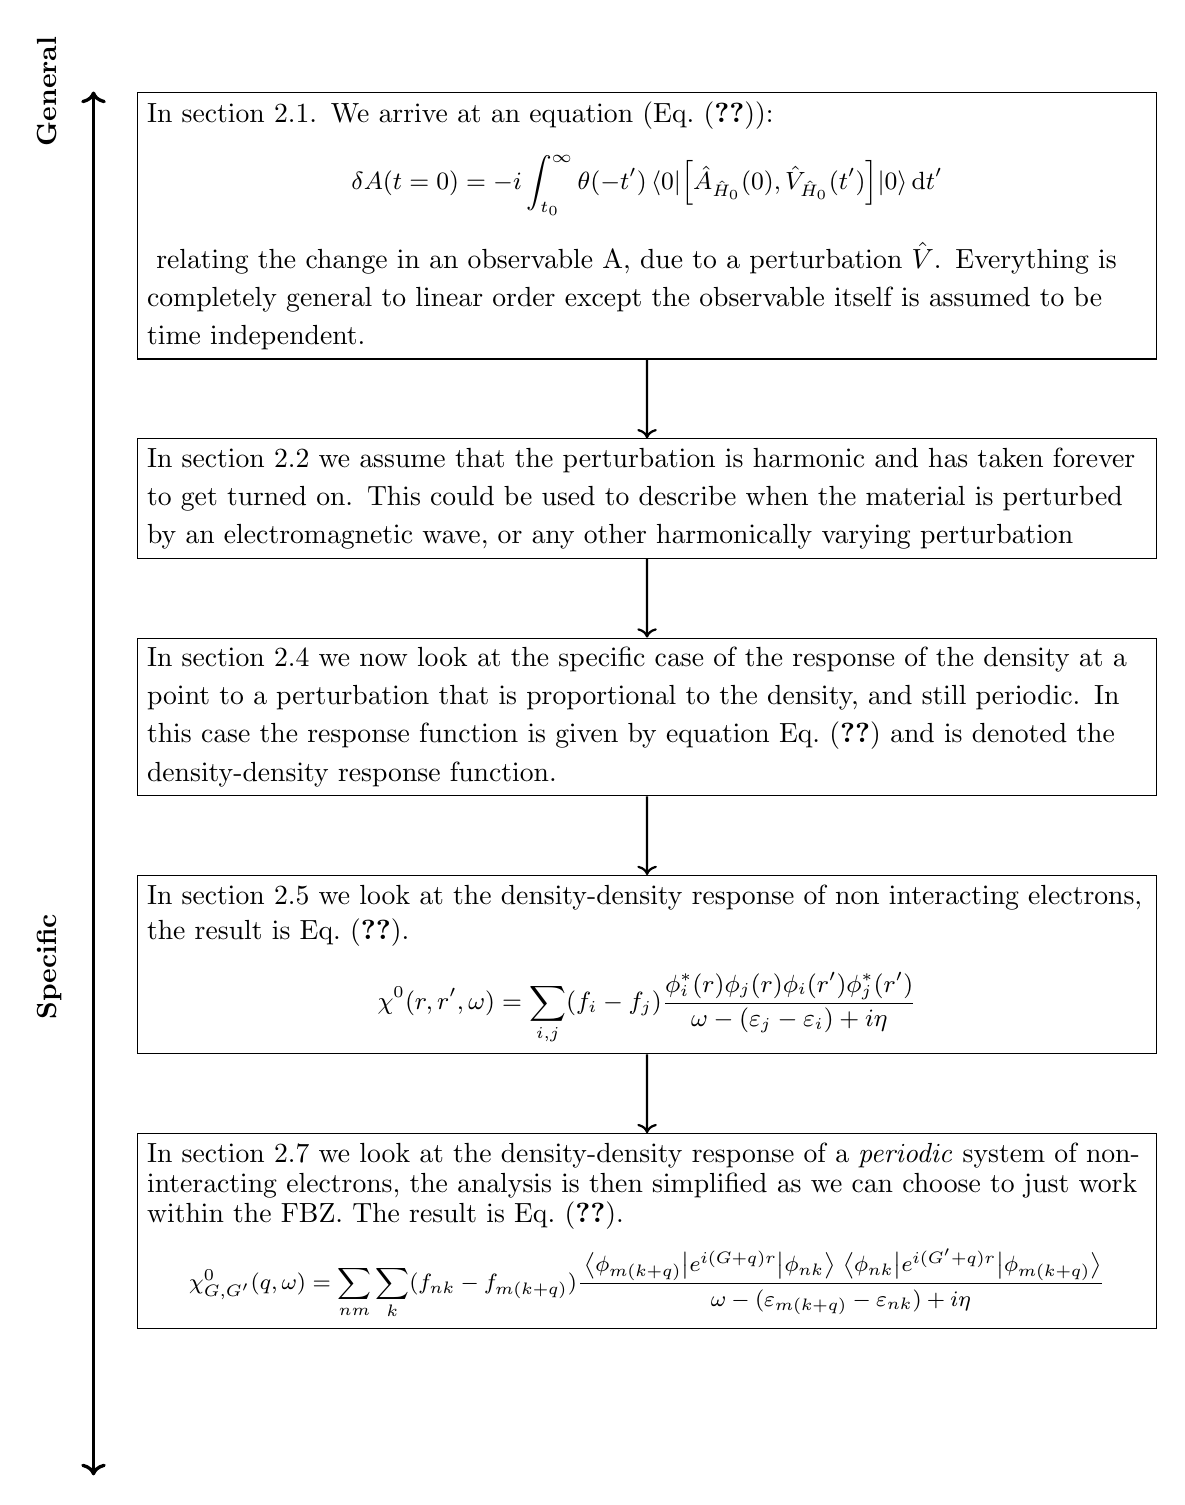
\begin{tikzpicture}[scale=0.95]
% Boxes describing the different segments in chapter
% Chapter 2.1
\node [minimum width = 12.9cm,below,text width=12.7cm] (A) at (-5.1,10) [draw, align=left] {In section 2.1. We arrive at an equation (\eqref{eq:Sol:21}): {\small \[ \delta A(t=0) = - i \int_{t_0}^{\infty} \theta(-t') \mel{0}{\comm{\hat{A}_{\hat{H}_0}(0)}{ \hat{V}_{\hat{H}_0}(t')}}{0} \text{d}t' \]} relating the change in an observable A, due to a perturbation $\hat{V}$. Everything is completely general to linear order except the  observable itself is assumed to be time independent.};

% Chapter 2.2 at (-5.1,7.88) [draw, align=left]
\node [below = of A,minimum width = 12.9cm,text width=12.7cm,draw,align=left] (B) {In section 2.2 we assume that the perturbation is harmonic and has taken forever to get turned on. This could be used to describe when the material is perturbed by an electromagnetic wave, or any other harmonically varying perturbation} ;

%Chapter 2.4
\node [below = of B,minimum width = 12.9cm,below,text width=12.7cm,draw,align=left] (C) {In section 2.4 we now look at the specific case of the response of the density at a point to a perturbation that is proportional to the density, and still periodic. In this case the response function is given by equation \eqref{eq:densitydensity} and is denoted the density-density response function.};

%Chapter 2.5
\node [below = of C,minimum width = 12.9cm,below,text width=12.7cm,draw,align=left] (D) {In section 2.5 we look at the density-density response of non interacting electrons, the result is \eqref{eq:234}. {\small \[ \chi^{0}(r,r',\omega) = \sum_{i,j} (f_i-f_j)\dfrac{\phi^{*}_i(r)\phi_j(r)\phi_i(r')\phi^{*}_j(r')}{\omega - (\varepsilon_j - \varepsilon_i) + i\eta} \]}};


%Chapter 2.7
\node [below = of D,minimum width = 12.9cm,below,text width=12.7cm,draw,align=left] (E) {In section 2.7 we look at the density-density response of a \textit{periodic} system of noninteracting electrons, the analysis is then simplified as we can choose to just work within the FBZ. The result is \eqref{eq:247}. {\footnotesize \[ \chi_{G,G'}^{0}(q,\omega) = \sum_{nm} \sum_{k} (f_{nk}-f_{m(k+q)}) \frac{\mel{\phi_{m(k+q)}}{e^{i(G+q)r}}{\phi_{nk}}\mel{\phi_{nk}}{e^{i(G'+q)r}}{\phi_{m(k+q)}}}{\omega - (\varepsilon_{m(k+q)}-\varepsilon_{nk})+i\eta}  \]}};

\draw[->,thick, to path={-- (\tikztotarget)}]
  (A) edge (B) (B) edge (C) (C) edge (D) (D) edge (E);

%% Axis describing generality and specific
\draw[<->, very thick] (-12.5,-8.5) -- (-12.5,10);
\node at (-13,10)  [rotate=90, anchor = base]  {\textbf{General}};
\node at (-13,-1.7) [rotate=90, anchor = base]  {\textbf{Specific}};
\end{tikzpicture}



\end{figure}
\end{solution}
\newpage \section{Week 3 \& 4: Dielectric function}
\subsection{Section 1; Time-dependent Hartree theory}
\begin{exercise}
Given the following induced density functionals
\begin{align}
    \delta n(r,\omega) &= \int \chi^{0}(r,r',\omega)\delta v_s(r',\omega)\mathrm{d}r' \quad  \text{induced density due to effective potential}\label{eq:301}\\
    \delta v_s(r,\omega) &= v_{ext}(r,\omega) + \int \dfrac{\delta n(r',\omega)}{\abs{r-r'}}\mathrm{d}r' \: \text{effective potential} \label{eq:302}\\
    \delta n(r,\omega) &= \int \chi(r,r',\omega)v_{ext}(r',\omega)\mathrm{d}r' \quad\text{real induced potential} \label{eq:303}
\end{align}
Show that the real and effective density response functions are related via
\begin{equation}
    \chi(r,r',\omega) = \chi^{0}(r,r',\omega) + \int\int \chi^{0}(r,r_1,\omega) \dfrac{1}{\abs{r_1-r_2}}\chi(r_2,r',\omega)\mathrm{d}r_1\mathrm{d}r_2
\end{equation}
\end{exercise}
\begin{solution}
The goal is to relate $\chi^{0}$ and $\chi$ through setting equations (\ref{eq:301}) and (\ref{eq:303}) equal. They are not generally equal, but will show when the two expressions are equal. In summary we must require that: 
\begin{equation}
    \int \chi^{0}(r,r',\omega)\delta v_s(r',\omega)\mathrm{d}r' = \int \chi(r,r',\omega)v_{ext}(r',\omega)\mathrm{d}r'
    \label{eq:35}
\end{equation}
Hence we will start by substituting the effective potential from \eqref{eq:302} in \eqref{eq:301}, keeping careful track of the $r$-notation:
Now only looking at the LHS of \eqref{eq:35} we can insert \eqref{eq:302} to get
\begin{equation}
   \mathrm{LHS} = \int \chi^{0}(r,r',\omega)v_{ext}(r',\omega) \mathrm{d}r' + \int\int \chi^{0}(r,r',\omega)\dfrac{\delta n(r'',\omega)}{\abs{r'-r''}}\mathrm{d}r''\mathrm{d}r'
\end{equation}
Now substituting $\delta n(r'',\omega)$ with \eqref{eq:303} to get
{\small
\begin{equation}
   \int \chi^{0}(r,r',\omega)v_{ext}(r',\omega) \mathrm{d}r' + \int\int\int \chi^{0}(r,r',\omega)\dfrac{1}{\abs{r'-r''}}\chi(r'',r''',\omega)v_{ext}(r''',\omega)\mathrm{d}r'''\mathrm{d}r''\mathrm{d}r'
\end{equation}}
In the last term we now change the notation by $r' \rightarrow r_1$ , $r'' \rightarrow r_2$. $r''' \rightarrow r'$.
\begin{equation}
   \int \left( \chi^{0}(r,r',\omega)v_{ext}(r',\omega) + \int\int \chi^{0}(r,r_1,\omega)\dfrac{1}{\abs{r_1-r_2}}\chi(r_2,r',\omega)v_{ext}(r',\omega)\mathrm{d}r_2\mathrm{d}r_1 \right) \mathrm{d}r'
\end{equation}
The RHS remains the same and we may obtain the solution, by differentiating once (to lift the integral over $r'$) and dividing by $v_{ext}(r',\omega)$. Thus
\begin{equation}
    \chi(r,r',\omega) = \chi^{0}(r,r',\omega) + \int\int \chi^{0}(r,r_1,\omega) \dfrac{1}{\abs{r_1-r_2}}\chi(r_2,r',\omega)\mathrm{d}r_1\mathrm{d}r_2
\end{equation}
\end{solution}

\subsection{Section 2; The exchange-correlation kernel}
\begin{exercise}
Given the definition of the density response of an  interacting electron system, $\chi$, and a non-interacting Kohn-Sham system, $\chi^{s}$, given by:
\begin{align}
    \chi(r,r',t-t') &= \left.\dfrac{\delta n(r,t)}{\delta v_{ext}(r',t')}\right|_{n_0(r)} \label{eq:310}\\
    \chi^{s}(r,r',t-t') &= \left.\dfrac{\delta n(r,t)}{\delta v_{s}(r',t')}\right|_{n_0(r)}
    \label{eq:311}
\end{align}
Use the chain rule of functional differentiation to derive the following relation
\begin{equation}
\begin{split}
    \chi(r,r',\omega) =& \chi^{s}(r,r',\omega)+ \\&\int\int \chi^{s}(r,r_1,\omega)\left[ \dfrac{1}{\abs{r_1-r_2}} + f_{xc}[n](r_1,r_2,\omega)\right]\chi(r_2,r',\omega)\mathrm{d}r_1\mathrm{d}r_2
\end{split}
\end{equation}
where 
\begin{equation}
    f_{xc}[n](r,r',t-t') = \dfrac{\delta v_{xc}[n](r,t)}{\delta n(r',t')}\label{eq:313}
\end{equation}
\end{exercise}

\begin{solution}
Using the general time dependent Hartree Fock result for the effective potential
\begin{equation}
    v_s(r,t) = v_{ion}(r) + \int \frac{n(r',t)}{\abs{r-r'}} \mathrm{d}r' + v_{ext}(r,t) + v_{xc}(r,t)
    \label{eq:314}
\end{equation}
The chain rule of functional derivatives states
\begin{equation}
    \frac{\delta F[Y]}{\delta X(r)} = \int \mathrm{d}s \frac{\delta F[Y]}{\delta Y(s)} \frac{\delta Y(s)}{\delta X(r)}
    \label{eq:315}
\end{equation}
We start off by evaluating the functional derivative in \eqref{eq:310}.
\begin{equation}
   \chi(r,r',t-t') =  \dfrac{\delta n(r,t)}{\delta v_{ext}(r',t')} = \int \dfrac{\delta v_s(r_1,t_1)}{\delta v_{ext}(r,t)}\dfrac{\delta n(r,t)}{\delta v_{s}(r_1,t_1)}\mathrm{d}r_1\mathrm{t_1}
    \label{eq:316}
\end{equation}
We immediately note that the second fraction on the RHS corresponds to $\chi^{s}(r,r_1,t-t_1)$. The remaining term we further expand using \eqref{eq:314}.
{\small
\begin{equation}
    \dfrac{\delta n(r,t)}{\delta v_{ext}(r',t')} = \int \chi^{s}(r,r_1,t-t_1) \left[\dfrac{\delta v_{ext}(r_1,t_1)}{\delta v_{ext}(r',t')} + \dfrac{\delta v_H(r_1,t_1)}{\delta v_{ext}(r',t')} + \dfrac{\delta v_{xc}(r_1,t_1)}{\delta v_{ext}(r',t')} + \dfrac{\delta v_{ion}(r_1,t_1)}{\delta v_{ext}(r',t')} \right]\mathrm{d}r_1\mathrm{t_1}
    \label{eq:317}
\end{equation}}
Where $v_H$ is the Hartree term (second term in RHS of \eqref{eq:314}). The first functional derivative above evaluates to a delta function, as
\begin{equation}
    \dfrac{\delta v_{ext}(r_1,t_1)}{\delta v_{ext}(r',t')} = \delta(r_1-r') \delta(t_1-t')
\end{equation}
The second term (Hartree), is evaluated using the chain rule again
\begin{equation}
    \dfrac{\delta v_H(r_1,t_1)}{\delta v_{ext}(r',t')} = \int \dfrac{\delta v_H(r_1,t_1)}{\delta n(r_2,t_2)} \dfrac{\delta n(r_2,t_2)}{\delta v_{ext}(r',t')}      \mathrm{d} r_2 \mathrm{d} t_2 = \int \dfrac{1}{\abs{r_1 - r_2}}\chi(r_2,r',t_2-t')\mathrm{d}r_2\mathrm{d}t_2
\end{equation}
We again use the chain rule to evaluate the third term
{\small
\begin{equation}
    \dfrac{\delta v_{xc}(r_1,t_1)}{\delta v_{ext}(r',t')} = \int \dfrac{\delta v_{xc}(r_1,t_1)}{\delta n(r_2,t_2)} \dfrac{\delta n(r_2,t_2)}{\delta v_{ext}(r',t')} \mathrm{d}r_2\mathrm{d}t_2 = \int f_{xc}(r_1,r_2,t_2-t_1) \chi(r_2,r',t_2-t') \mathrm{d}r_2\mathrm{d}t_2
\end{equation}}
where the first fraction on the RHS is $f_{xc}(r_1,r_2,t_1-t_2)$ from \eqref{eq:313}, and the second fraction is $\chi(r_2,r',t_2-t')$. The term with $v_{ion}$ is zero, as we have previously assumed the ions to be stationary, hence the potential will not change due to any external field. Collecting everything the full functional derivative becomes
\begin{equation}
\begin{split}
\dfrac{\delta n(r,t)}{\delta v_{ext}(r',t')} 
= & \int \chi^{s}(r,r_1,t-t_1) \left[\delta(r_1-r') \delta(t_1-t') +  \int \dfrac{1}{\abs{r_1 - r_2}}\chi(r_2,r',t_2-t')\mathrm{d}r_2\mathrm{d}t_2  \right.\\ &\left. +  \int f_{xc}(r_1,r_2,t_2-t_1) \chi(r_2,r',t_2-t') \mathrm{d}r_2\mathrm{d}t_2 \right] \mathrm{d}r_1 \mathrm{d}t_1
\end{split}
\end{equation}
{\small
\begin{equation}
    \begin{split}
\chi(r,r',t-t') &= \dfrac{\delta n(r,t)}{\delta v_{ext}(r',t')} 
= \chi^{s}(r,r',t-t')  + \\&\int \int \chi^{s}(r,r_1,t-t_1)\left[\dfrac{1}{\abs{r_1 - r_2}}    +  f_{xc}(r_1,r_2,t_2-t_1) \right]\chi(r_2,r',t_2-t') \mathrm{d}r_2\mathrm{d}t_2\mathrm{d}r_1 \mathrm{d}t_1
\end{split}
\end{equation}}
Fourier transforming the time dependence we see that all terms correspond to convolutions (Unsure why this applies) so that we obtain:
\begin{equation}
    \chi(r,r',\omega) = \chi^{s}(r,r',\omega)  + \int \int \chi^{s}(r,r_1,\omega)\left[\dfrac{1}{\abs{r_1 - r_2}}    +  f_{xc}(r_1,r_2,\omega) \right]\chi(r_2,r',\omega) \mathrm{d}r_2\mathrm{d}r_1
\end{equation}
\end{solution}


\subsection{Section 3; The dielectric function}
\begin{exercise}
Show that the inverse dielectric function is given by
\begin{equation}
    \epsilon^{-1}(r,r',\omega) = \delta(r-r') + \int \dfrac{1}{\abs{r-r_1}}\chi(r_1,r',\omega)\mathrm{d}r_1
\end{equation}
\end{exercise}
\begin{solution}
First equation 17 and 18 from the problem handout are set equal to each other 
\begin{equation}
    \delta v_{tot}(r,\omega) = \int \epsilon^{-1} v_{ext}(r_1,\omega) \mathrm{d} r_1 = v_{ext}(r,\omega) + \int \frac{\delta n(r_1,\omega)}{\abs{r-r_1}} \mathrm{d}r_1\label{eq:326}
\end{equation}
We then take the functional derivative of the above equation with respect to $v_{ext}(r',\omega)$
\begin{equation}
    \dfrac{\delta v_{tot}(r,\omega)}{\delta v_{ext}(r',\omega)} = \dfrac{\delta v_{ext}(r,\omega)}{\delta v_{ext}(r',\omega)} + \int \dfrac{1}{\abs{r-r_1}}\dfrac{\delta n(r_1,\omega)}{\delta v_{ext}(r',\omega)}\mathrm{d}r_1
\end{equation}

the first term in the RHS just evaluates to a delta function $\delta(r-r')$. The functional derivative in the integral is just the definition of $\chi$ evaluated at $\chi(r_1,r',\omega)$, so we obtain:
\begin{equation}
    \dfrac{\delta v_{tot}(r,\omega)}{\delta v_{ext}(r',\omega)} = \delta(r-r') + \int \dfrac{1}{\abs{r-r_1}}\chi(r_1,r',\omega)\mathrm{d}r_1 \label{eq:327}
\end{equation}
Now we repeat the operation on the middle term in \eqref{eq:326}, which somewhat trivially reduces to:
\begin{equation}
    \dfrac{\delta v_{tot}(r,\omega)}{\delta v_{ext}(r',\omega)} = \int \epsilon^{-1}\dfrac{\delta v_{ext}(r_1,\omega)}{\delta v_{ext}(r',\omega)} \mathrm{d}r_1 = \int \epsilon^{-1} \delta(r_1 - r') \mathrm{d}r_1 = \epsilon^{-1} \label{eq:328}
\end{equation}
Thus it all reduces to
\begin{equation}
    \epsilon^{-1}(r,r',\omega) = \delta(r-r') + \int \dfrac{1}{\abs{r-r_1}}\chi(r_1,r',\omega) \mathrm{d}r_1
\end{equation}
\end{solution}

%%%
\begin{exercise}
When exchange and correlation effects are neglected, i.e. within the RPA, the total potential $\delta v_{tot}$ becomes identical to the effective potential $\delta v_s$. In that case show that the dielectric function is given in real space by
\begin{equation}
    \epsilon(r,r',\omega) = \delta(r-r') + \int \dfrac{1}{\abs{r-r_1}}\chi^{0}(r_1,r',\omega)\mathrm{d}r_1
\end{equation}
\end{exercise}
\begin{solution}
We start by isolating the inverse dielectric function from \begin{equation}
    \delta v_{tot} = \int\epsilon^{-1}(r,r',\omega)v_{ext}(r',\omega)\mathrm{d}r'
\end{equation}
by taking the functional derivative with respect to $\delta v_{ext}(r'',\omega)$ so that
\begin{equation}
    \dfrac{\delta v_{tot}(r)}{\delta v_{ext}(r'')} = \int\epsilon^{-1}(r,r',\omega)\delta(r'-r'')\mathrm{d}r' = \epsilon^{-1}(r,r',\omega)
\end{equation}
From the above we may flip the relation so that
\begin{equation}
    \dfrac{\delta v_{ext}(r')}{\delta v_{tot}(r)} = \epsilon(r,r',\omega)
\end{equation}
In the case where exchange and correlation effects are neglected $\delta v_{tot}$ takes the form of \eqref{eq:314} with $v_{xc} = 0$. As the ionic potential doesn't change with applied fields (frozen in approximation) the only terms are the Hatree term and the external potential. Isolating the external potential in \eqref{eq:314} and using the adiabatic property (of turning on the potential at negative infinity)\footnote{so that $\delta v_{tot} = \delta v_{ext} + \int \delta n(r',\omega)/\abs{r-r'}\mathrm{d}r'$} we obtain:
\begin{equation}
\begin{split}
    \dfrac{\delta v_{ext}(r')}{\delta v_{tot}(r)} &= \dfrac{\delta v_{tot}(r')}{\delta v_{tot}(r)} - \int \dfrac{\delta n(r_1,\omega)}{\delta v_{tot}(r)}\dfrac{1}{\abs{r-r_1}}\mathrm{d}r_1
    \\&= \delta(r-r') - \int \dfrac{1}{\abs{r'-r_1}}\chi^{0}(r_1,r',\omega)\mathrm{d}r_1 = \epsilon(r,r',\omega)
\end{split}
\end{equation}
where we may shift the indexes of $r' \leftrightarrow r$ on the LHS to obtain the solution.
\end{solution}

\subsection{Section 4; the scalar macroscopic dielectric function}
\begin{exercise}
Argue why the scalar macroscopic dielectric function $\epsilon_M(\omega)$ given by:
\begin{equation}
    \epsilon_M(\omega) = \lim_{q\rightarrow 0} \dfrac{1}{\epsilon_{00}^{-1}(q,\omega)}
\end{equation} 
is in general different from $\lim_{q\rightarrow 0} \epsilon_{00}(q,\omega)$. When does it hold that \\ $\epsilon_M = \lim_{q\rightarrow 0} \epsilon_{00}(q,\omega)$?
\end{exercise}
\begin{solution}
Start by recalling that the dielectric function relates the external potential to the total potential through:
\begin{equation}
    \delta v_{tot}(r,\omega) = \int \epsilon^{-1}(r,r',\omega)v_{ext}(r',\omega)\mathrm{d}r'
\end{equation}
If we consider the discretised version of the above equation in reciprocal space the dielectric function has the matrix form:
\begin{equation}
    \underline{\underline{\epsilon}} = \begin{bmatrix}
    \underline{\underline{\epsilon_{00}}} & \underline{\underline{\epsilon_{01}}} &.&.&.\\
    \underline{\underline{\epsilon_{10}}} & \underline{\underline{\epsilon_{11}}} & & & \\
    .& &.& & & \\
    .& & &.& & \\
    .& & & &.& \\
    \end{bmatrix}
\end{equation}
where the matrices inside the matrices represent the discretised momentum coordinate $q$, and the corresponding external potential has the form:
\begin{equation}
   \underline{v_{ext}} = [v(G=0,q=0),v(G=0,q_1),v(G=0,q_2),...,v(G=1,q=0),...]^{\mathrm{T}} 
\end{equation}
Evidently, as we are interested in the change in the total potential due to an external field, we must take the form desired element of $\epsilon^{-1}$ rather than $\epsilon$ as the relation $(\underline{\underline{A}}[1,1])^{-1} = \underline{\underline{A}}^{-1}[1,1]$ is only true for diagonal matrices. We must further focus on the $\epsilon_{00}$ element as we are interested in the change due to "slow"-varying field, such as optical frequencies. Consequently taking the limit $\epsilon_M = \lim_{q\rightarrow 0} \epsilon_{00}(q,\omega)$ would change the question from: \emph{"how is the total potential influence by an external potential"} to \emph{"what external potential would generate this change in the total potential"}.
\end{solution}
\newpage \section{Week 5: Plasmons}

\subsection{Section 1; Second quantized Coulomb interaction}
\begin{exercise}
Use the fact that
\begin{equation}
    \dfrac{1}{\Omega} \int \dfrac{\mathrm{e}^{irk}\mathrm{e}^{-ir'k'}}{\abs{r-r'}}\mathrm{d}r\mathrm{d}r' = \delta_{kk'} \frac{4 \pi}{k^2}
\end{equation}
to derive the second quantized form of the Coulomb interaction, $\hat{H}_{int}$, given by
\begin{equation}
    \hat{H}_{int} = \dfrac{1}{2\Omega}\sum_q\sum_{k,k'}V_q c^{\dagger}_{k}c^{\dagger}_{k'}c_{k'+q}c_{k-q}
\end{equation}
where $V_q = 4\pi/q^2$.
\end{exercise}
\begin{solution}
We start by recalling that a second quantized operator can be obtained from GP (B.12):
\begin{equation}
    \hat{Q} = \dfrac{1}{2}\sum_{k,k',q,q'} \mel{\psi_k\psi_q}{\dfrac{1}{r}}{\psi_{k'} \psi_{q'}}c^{\dagger}_{k}c^{\dagger}_{k'}c_{q}c_{q'}
\end{equation}
As it is assumed that the system is homogeneous, i.e. translational invariant, the states are spanned by plane waves of the form $\ket{k} = \Omega^{-1/2}\mathrm{e}^{ikr}$ we may write
\begin{equation}
    \hat{H}_{int} = \dfrac{1}{2\Omega^2}\sum_{k,k',q,q'}\int\int\e^{-ikr}\e^{-ik'r'}\dfrac{1}{\abs{r-r'}}\e^{iqr}\e^{iq'r'}\mathrm{d}r\mathrm{d}r'c^{\dagger}_{k}c^{\dagger}_{k'}c_{q}c_{q'}
\end{equation}
Combining the exponentials in $r$ and $r'$ we get it on the form of the fact that we are to use
\begin{equation}
   \frac{1}{\Omega} \int\int\e^{-ikr}\dfrac{1}{\abs{r-r'}}\e^{ik'r'}\mathrm{d}r\mathrm{d}r' = \delta_{k,k'}\dfrac{4\pi}{k^2}
\end{equation}
so that
\begin{equation}
\begin{split}
    \hat{H}_{int} &= \dfrac{1}{2\Omega^2}\sum_{k,k',q,q'} \int\int\e^{-i(k-q)r}\dfrac{1}{\abs{r-r'}}\e^{i(q'-k')r'}\mathrm{d}r\mathrm{d}r'c^{\dagger}_{k}c^{\dagger}_{k'}c_{q}c_{q'} \\
    &= \dfrac{1}{2\Omega}\sum_{k,k',q,q'}\delta_{k-q,q'-k'}\dfrac{4\pi}{Q^2}c^{\dagger}_{k}c^{\dagger}_{k'}c_{q}c_{q'}
\end{split}
\end{equation}
where the Kronecker delta function corresponds to conservation of momentum (which must be true given a translational invariant system). From this we may obtain an expression for $q' = k'+k-q$. Shifting the index $q_1 \rightarrow k-q$ leads to $q' = k' + q$. Evaluating $Q^2 = (k-q)(q'-k') = (k-q)^2 = q_1^2$. Renaming $q_1 \rightarrow q$ we obtain the solution
\begin{equation}
    \hat{H}_{int} = \dfrac{1}{2\Omega}\sum_{q}\sum_{k,k'}\dfrac{4\pi}{q^2}c^{\dagger}_{k}c^{\dagger}_{k'}c_{k'+q}c_{k-q} = \dfrac{1}{2\Omega}\sum_{q}\sum_{k,k'}V_q c^{\dagger}_{k}c^{\dagger}_{k'}c_{k'+q}c_{k-q}
\end{equation}
In the remainder we have let $\frac{V_q}{2 \Omega}\rightarrow V_q$
Q.E.D.
\end{solution}

\subsection{Section 2; Equation of motion method (EOM)}
\begin{exercise}
Show that $\hat{S}_{i}^{\dagger} = \ket{E_i}\bra{E_0}$ satisfy the commutation relation
\begin{equation}\label{eq:4e2}
    \comm{\hat{H}}{\hat{S}_{i}^{\dagger}} = (E_i - E_0)\hat{S}_{i}^{\dagger} \: \textrm{and} \: \comm{\hat{S}_{i}}{\hat{H}} = (E_i - E_0)\hat{S}_{i} 
\end{equation}
\end{exercise}

\begin{solution}
The commutator is given by
\begin{equation}
    \comm{\hat{H}}{\hat{S}_{i}^{\dagger}} = \hat{H} \hat{S}_i^{\dagger} \ket{E_0} - \hat{S}_i^{\dagger} \hat{H} \ket{E_0} = (E_i-E_0) \ket{E_i} = (E_i-E_0) \hat{S}_i^{\dagger} \ket{E_0}
\end{equation}
\end{solution}

\subsection{Section 3; RPA, Excitation operator}

\begin{exercise}
    We now introduce a set of simple excitation operators defined as,
    \begin{align}
        \hat{S}_k^{\dagger}(q) = c_{k+q}^{\dagger} c_k \\
        \hat{S}_k(q) = c_{k}^{\dagger} c_{k+q}
    \end{align}
    This operator creates a single electron-hole pair of momentum $q$. Show that \\$ \hat{S}_k^{\dagger}(q) \ket{E_0}$ is an eigenstate of $\hat{H}_0$, and  that the commutator with  $\hat{H}_0$ is given
by
\begin{equation}
    \comm{\hat{S}_k(q)}{\hat{H}_0} = (\varepsilon_{k+q}-\varepsilon_k) \hat{S}_k(q)
\end{equation}
\end{exercise}



\begin{solution}
Applying $\hat{H}_0$ on $ \hat{S}_k^{\dagger}(q) \ket{E_0}$ gives
\begin{equation}
    \hat{H}_0 \hat{S}_k^{\dagger}(q) \ket{E_0} = \sum_k \varepsilon_k c_k^{\dagger} c_k c_{k'+q}^{\dagger} c_{k'} \ket{E_0} = \sum_k \varepsilon_k c_k^{\dagger} c_k \ket{E_0}_{k'}^{k'+q}
\end{equation}
Where the subscript (superscript) on the state denotes that an electron has been removed (added) in the state. Here it is important to note that $\ket{E_0}$ is the Fermi sea containing many different states. So that 
\begin{equation}
     \hat{H}_0 \hat{S}_k^{\dagger}(q) \ket{E_0} =  \hat{H}_0 \ket{E_0}_{k'}^{k'+q} = \sum_k \varepsilon_k c_k^{\dagger} c_k \ket{E_0}_{k'}^{k'+q} = (E_{FS} + \varepsilon_{k'+q} - \varepsilon_{k'})\ket{E_0}_{k'}^{k'+q}
\end{equation}
So that $ \hat{S}_k^{\dagger}(q) \ket{E_0}$ is indeed an eigenstate of $\hat{H}_0$. \\
The commutator is found by acting on a state $\ket{E_0}$
\begin{equation}
   (\hat{S}_k \hat{H}_0 - \hat{H}_0 \hat{S}_k) \ket{E_0} = (E_{FS} - (E_{FS} +\varepsilon_{k} - \varepsilon_{k+q})) \ket{E_0}_{k+q}^k = (\varepsilon_{k+q} - \varepsilon_{k}) \hat{S}_k \ket{E_0}
\end{equation}
So that the commutator is indeed
\begin{equation}
    \comm{\hat{S}_k(q)}{\hat{H}_0} = (\varepsilon_{k+q}-\varepsilon_k) \hat{S}_k(q)
\end{equation}
\end{solution}




\begin{exercise}
Insert the exact excitation operator of the form
\begin{equation}
    \hat{S}(q) = \dfrac{1}{\sqrt{N}}\sum_k \phi_k(q)\hat{S}_k(q)
    \label{eq:417}
\end{equation}
into the defining equation (\eqref{eq:4e2}, right) to obtain 
\begin{equation}
    \dfrac{1}{\sqrt{N}}\sum_k \hat{S}_k(q) \left[(\omega(q) - (\varepsilon_{k+q}-\varepsilon_k))\phi_k(q) - V_{q}\sum_{k'}(f_{k'}-f_{k'+q})\phi_{k'}(q) \right] = 0
\end{equation}
\end{exercise}

\begin{solution}
In order to plug into \eqref{eq:4e2} we first note that 
\begin{equation}
    \comm{\hat{S}(q)}{\hat{H}} = \comm{\dfrac{1}{\sqrt{N}}\sum_k \phi_k(q)\hat{S}_k(q)}{\hat{H}} = \dfrac{1}{\sqrt{N}}\sum_k\phi_{k}(q) \comm{\hat{S}_k(q)}{\hat{H}}
\end{equation}
As the resulting sum of commutators is known from exercise 4.3.1, and yields 
\begin{equation}
    \comm{\hat{S}_k(q)}{\hat{H}} = (\varepsilon_{k+q}-\varepsilon_{k})\hat{S}_{k}(q)=\omega(q)\hat{S}_{k}(q)
\end{equation}
where the interaction energy of the excitation is labelled $\omega(q)$. So that the commutator of the real interaction operator becomes
\begin{equation}\label{eq:421}
    \comm{\hat{S}(q)}{\hat{H}} = \dfrac{1}{\sqrt{N}}\sum_k\phi_{k}(q) \omega(q)\hat{S}_k(q)
\end{equation}
The commutator in \eqref{eq:4e2} can be split into two commutators by
\begin{equation}\label{eq:422}
    \comm{\hat{S}}{\hat{H}} = \comm{\hat{S}}{\hat{H}_0} + \comm{\hat{S}}{\hat{H}_{int}}
\end{equation}
The commutator with the interacting Hamiltonian is given in equation (16) in the problem handout.
\begin{equation}
    \comm{\hat{S}_{k}}{\hat{H}_{int}} = V_q (f_k - f_{k+q}) \sum_{k'} \hat{S}_{k'}(q)
\end{equation}
Hence the commutator with the total interaction operator becomes
\begin{equation}\label{eq:424}
    \comm{\hat{S}}{\hat{H}_{int}} = \dfrac{1}{\sqrt{N}}\sum_{k} V_q (f_k - f_{k+q}) \phi_k(q) \sum_{k'} \hat{S}_{k'}(q)
\end{equation}
The sums over $k$ and $k'$ runs over the same elements, therefore the two indexes can be exchanged, so we choose to rename them by $k \leftrightarrow k'$, so
\begin{equation}\label{eq:425}
    \comm{\hat{S}}{\hat{H}_{int}} = \dfrac{1}{\sqrt{N}}\sum_{k'} V_q (f_{k'} - f_{k'+q}) \phi_k'(q) \sum_{k} \hat{S}_{k}(q)
\end{equation}
Now for the other commutator \\
The commutator $\comm{\hat{S}}{\hat{H}_0}$ is found by
\begin{equation}
    \comm{\hat{S}}{\hat{H}_0}\ket{E_i} = (\hat{S} \hat{H}_0-\hat{H}_0 \hat{S}) \ket{E_i} = (E_i - \hat{H}_0) \hat{S} \ket{E_i} 
\end{equation}
Inserting \eqref{eq:417} we obtain
\begin{align}
    \comm{\hat{S}}{\hat{H}_0}\ket{E_i} &= \frac{1}{\sqrt{N}}\sum_k (E_i - \hat{H}_0) \phi_k \hat{S}_k(q) \ket{E_i}  \\ 
    &= \frac{1}{\sqrt{N}}\sum_k (E_i - (E_i-\varepsilon_{k+q}+\varepsilon_k)) \phi_k \hat{S}_k(q) \ket{E_i} \\&=
    \frac{1}{\sqrt{N}} \sum_k (\varepsilon_{k+q}-\varepsilon_k)
    \phi_k \hat{S}_k(q) \ket{E_i} \label{eq:428}
\end{align}
Inserting equations (\ref{eq:425}) and (\ref{eq:428}) into the RHS of equation (\ref{eq:422}), and (\ref{eq:421}) into the LHS of \eqref{eq:422}
{\small
\begin{equation}
    \dfrac{1}{\sqrt{N}}\sum_k\phi_{k}(q) \omega(q)\hat{S}_k(q) = \frac{1}{\sqrt{N}} \sum_k \hat{S}_{k}(q)\left( (\varepsilon_{k+q}-\varepsilon_k)
    \phi_k + V_q \sum_{k'} (f_{k'} - f_{k'+q}) \phi_{k'}(q)\right)
\end{equation}}
Subtracting the RHS and omitting the sum over $k$ we obtain the result:
\begin{equation}
    \dfrac{1}{\sqrt{N}}\sum_k\hat{S}_{k}(q)\left[\left(\omega(q) - (\varepsilon_{k+q}-\varepsilon_k)\right)\phi_{k}(q) - V_q  \sum_{k'}(f_{k'} - f_{k'+q}) \phi_{k'}(q) \right] = 0
\end{equation}
where we can write the expansion coefficients by the recursive formula
\begin{equation}\label{eq:432}
    \phi_{k}(q) = \dfrac{V_q}{\omega(q) - (\varepsilon_{k+q}-\varepsilon_k)}\sum_{k'}(f_{k'} - f_{k'+q}) \phi_{k'}(q)
\end{equation}

\end{solution}

\begin{exercise}
Assuming a finite system, i.e. a finite number of electrons and thus a finite number of allowed intraband transitions with $(f_{k} - f_{k+q}) = 1$, sketch the right hand side of the following equation (Eq. (19) in the handout) as a function of $\omega(q)$.
\begin{equation}\label{eq:433}
    1 = V_{q}\sum_{k} \dfrac{f_{k}-f_{k+q}}{\omega(q) - (\varepsilon_{k+q} - \varepsilon_k)}
\end{equation}
Compare with fig. 10 on page 254 in GP.
\end{exercise}



\begin{solution}
The energy follows the free particle dispersion relation, as the states are assumed to be plane waves, with the effective mass set to one. Thus the energy difference in the denominator is
\begin{equation}
   \varepsilon_{k+q} - \varepsilon_k = \frac{(k+q)^2}{2} - \frac{k^2}{2} = kq - \frac{q^2}{2}
\end{equation}
Which means the peaks, found when the denominator is zero, are equally spaced as a function of $\omega(q)$. 
There cannot be an infinite number of transitions, as q then would have to be large enough that we exit the FBZ. So at some point there must be a cutoff.
\begin{figure}[h!]
\centering
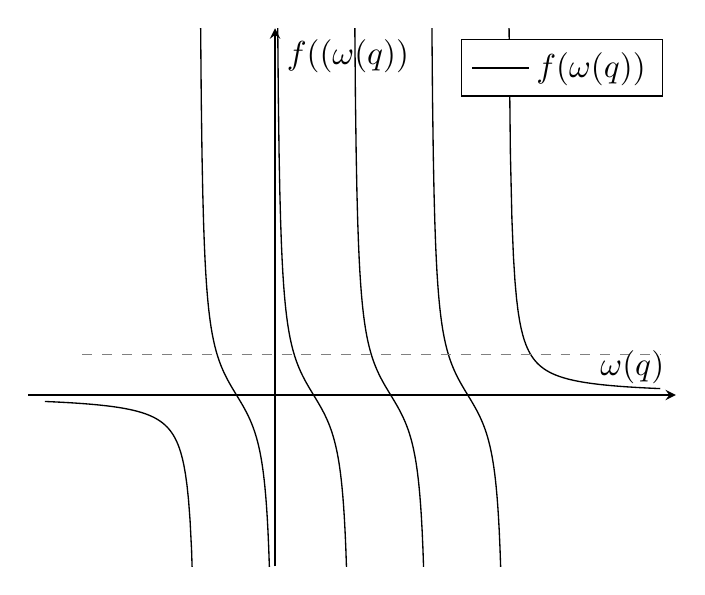
\begin{tikzpicture}[scale=1.2]
\begin{axis}[
    axis lines=middle,
    ticks=none,
    xmin=-2.5*pi,xmax=4.5*pi,ymin=-pi,ymax=8,
    xlabel={$\omega(q)$},
    ylabel={$f(\qty(\omega(q))$},
    domain=-10000:10000,
    restrict y to domain=-100000:100000,
    enlargelimits=true
    ]
% parts:
\addplot[black,domain=-3.1-2*pi:-0.01-pi,unbounded coords=jump,samples=101] {1/(x+pi)};
\addplot[black,domain=-3.1:-0.01,unbounded coords=jump,samples=101] {cot(deg(x))};
\addplot[black,domain=-3.1+pi:-0.01+pi,unbounded coords=jump,samples=101] {cot(deg(x))};
\addplot[black,domain=-3.1+2*pi:-0.01+2*pi,unbounded coords=jump,samples=101] {cot(deg(x))};
\addplot[black,domain=-3.1+3*pi:-0.01+3*pi,unbounded coords=jump,samples=101] {cot(deg(x))};
\addplot[black,domain=-3.1+4*pi:-0.01+5*pi,unbounded coords=jump,samples=101] {1/(x-3*pi)};

\addplot[dashed, black!50!white,domain=-2.5*pi:5*pi] {1};
\addlegendentry{$f\qty(\omega(q))$}
\end{axis}
\end{tikzpicture}
\end{figure}
\end{solution}

\begin{exercise}
Show that the solution for the expansion coefficients is given by
\begin{equation}\label{eq:435}
    \phi_k(q) = \dfrac{V_q}{\omega(q) - (\varepsilon_{k+q}-\varepsilon_{k})}
\end{equation}
\end{exercise}

\begin{solution}
Inserting the solution given above, \eqref{eq:435}, in the solution of exercise 4.3.2, given in \eqref{eq:432}, on the LHS we get
\begin{equation}
\begin{split}
    \phi_{k}(q) &= \dfrac{V_q}{\omega(q) - (\varepsilon_{k+q}-\varepsilon_k)}\sum_{k'}(f_{k'} - f_{k'+q}) \phi_{k'}(q) \\&= \dfrac{V_q}{\omega(q) - (\varepsilon_{k+q}-\varepsilon_k)}\sum_{k'}V_q\dfrac{f_{k'} - f_{k'+q}}{\omega(q) - (\varepsilon_{k'+q}-\varepsilon_k')}
\end{split}
\end{equation}
The solution must satisfy the transcendental equation, \eqref{eq:433}, for a solution to exist. Hence the sum over $k'$ must equal 1 and consequently the remaining term is the ansatz.
\end{solution}

\begin{exercise}
Sketch the form of this function and compare with the corresponding result for the finite system.
\begin{equation}
    \text{r.h.s. of Eq. (19)} = \mathrm{Re}\{\epsilon(q, \omega)\} \approx 1 - \dfrac{\alpha(q)}{\omega - (\langle\varepsilon_{k+q} - \varepsilon_{k}\rangle) + \gamma}
\end{equation}
where $\langle\varepsilon_{k+q} - \varepsilon_{k}\rangle$ denotes the average of the allowed non-interacting transition energies and $\gamma$ is a positive number.
\end{exercise}
\begin{solution}
As with the previous expression (Look in problem handout) we look for the case when the real part of the dielectric function vanishes, this is the case when
\begin{equation}
    1 = \frac{\alpha(q)}{\omega - \langle (\varepsilon_{k+q} - \varepsilon_k) \rangle + \gamma}
\end{equation}
This equation is sketched below:
\begin{figure}[h!]
\centering
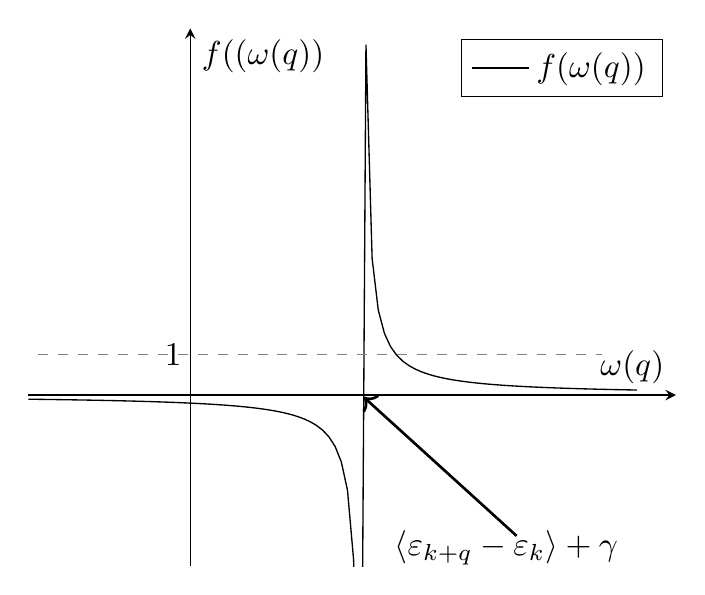
\begin{tikzpicture}[scale=1.2]
\begin{axis}[
    axis lines=middle,
    ticks=none,
    xmin=-1*pi,xmax=4*pi,ymin=-pi,ymax=8,
    xlabel={$\omega(q)$},
    ylabel={$f(\qty(\omega(q))$},
    domain=-10000:10000,
    restrict y to domain=-100000:100000,
    enlargelimits=true
    ]
% parts:
\addplot[black,domain=-5.1:13 ,unbounded coords=jump,samples=102] {1/(x-5)};
\node at (-0.5,1) {1};

\addplot[dashed, black!50!white,domain=-5:12] {1};
\addlegendentry{$f\qty(\omega(q))$}
\draw[->, thick] (9.5,-3.5) -- (5.05,-0.05);
\node at (9.2,-3.8) {$\langle \varepsilon_{k+q} - \varepsilon_k \rangle + \gamma$};
\end{axis}
\end{tikzpicture}
\end{figure}
\end{solution}

\newpage \section{Week 6 \& 7: Excitons}
\subsection{Section 1; Model}
\begin{exercise}
We are considering a simple two band model of a one dimensional semi-conductor. The valence and conduction band atomic orbitals of unit cell $n$ are denotes $\phi_{vn}\qty(r) = \phi_v\qty(r- R_N)$ and $\phi_{vn}\qty(r) = \phi_v\qty(r- R_N)$ respectively and satisfy the orthonormality relations, \ie, $\ip{\psi_{n,\alpha}}{\psi_{m,\beta}} = \delta_{nm}\delta{\alpha\beta}$ for $\alpha,\beta \in \{v,c\}$. The non-interacting part of the Hamiltonian takes the form: 
\begin{equation}
    \begin{split}
        H_0 =& \sum_n \varepsilon_v \crea{c}{nv} \anni{c}{nv} + t \qty(\crea{c}{nv} \anni{c}{n+1,v} + \crea{c}{nv}\anni{c}{n-1,v})\\
        +& \sum_n \varepsilon_c \crea{c}{nc} \anni{c}{nc} - t \qty(\crea{c}{nc} \anni{c}{n+1,c} + \crea{c}{nc}\anni{c}{n-1,c})\\
    \end{split}
\end{equation}
Calculate and sketch the band structure assuming that $\varepsilon_c - \varepsilon_v > 4t$. Express the gab in terms of the parameters of the model. Sketch the joint density of states and identify the critical points.
\end{exercise}

\begin{solution}
We let the Hamiltonian act on a Bloch state $\ket{k} = \sum_n e^{ikna} \ket{n}$ and otherwise follow the exact same approach as solution 1.2.2, the first term will only give contributions in the valence band, whereas the second will only give contributions in the conduction band, thereby we have from equation \ref{eq:114} that
\begin{equation}
\begin{split}
    \varepsilon_{valence} = \varepsilon_v + 2t\cos(ka) \\
    \varepsilon_{conduction} = \varepsilon_c - 2t\cos(ka)
    \end{split}
\end{equation}
As $\varepsilon_c - \varepsilon_v > 4t$ there is a bandgap.


\begin{figure}[!ht]
    \centering
    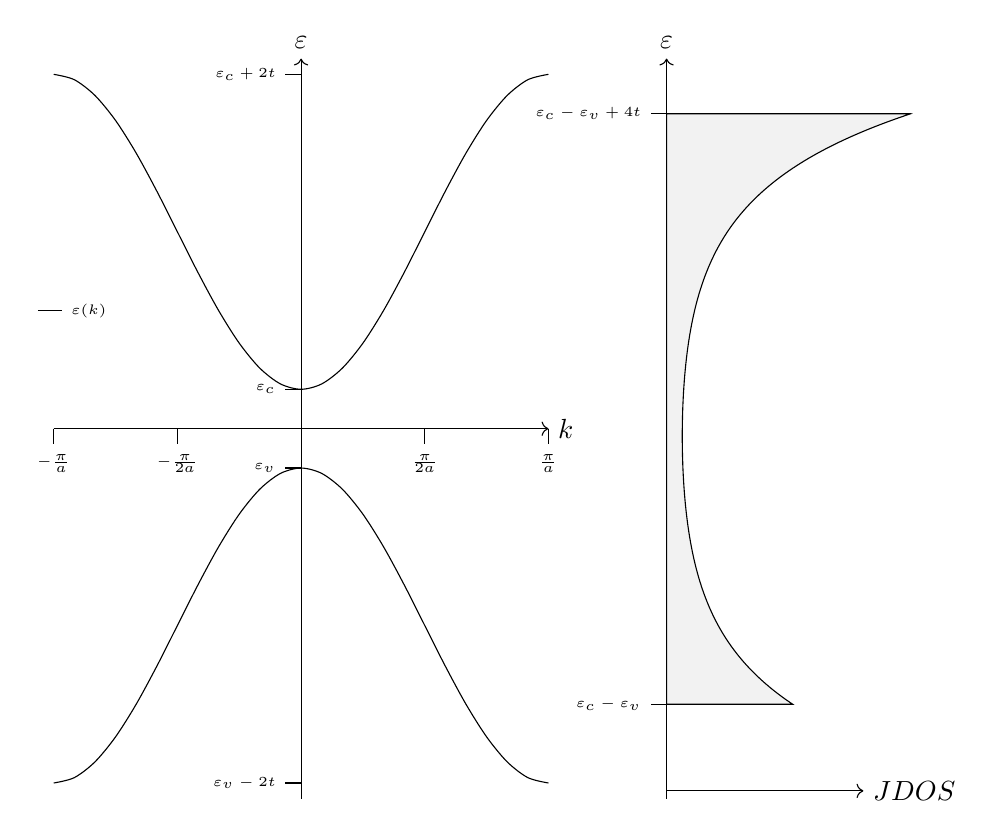
\begin{tikzpicture}
    % Axes
    \draw[->] (-pi,0) -- (pi,0) node[right] {$k$};
    \draw[->] (0,-4.7) -- (0,4.7) node[above] {$\varepsilon$};
    
    % Ticks
        %y
        \draw (0,4.5) -- (-0.2,4.5) node[left] {\tiny{$\varepsilon_c + 2t$}};
        \draw (0,0.5) -- (-0.2,0.5) node[left] {\tiny{$\varepsilon_c$}};
        \draw (0,-0.5) -- (-0.2,-0.5) node[left] {\tiny{$\varepsilon_v$}};
        \draw (0,-4.5) -- (-0.2,-4.5) node[left] {\tiny{$\varepsilon_v-2t$}};
        
        %x
        \draw (-pi,0)   -- (-pi,-0.2)    node[below] {\tiny{$-\frac{\pi}{a}$}};
        \draw (-pi/2,0) -- (-pi/2,-0.2)  node[below] {\tiny{$-\frac{\pi}{2a}$}};
        \draw (pi/2,0)  -- (pi/2,-0.2)   node[below] {\tiny{$\frac{\pi}{2a}$}};
        \draw (pi,0)    -- (pi,-0.2)     node[below] {\tiny{$\frac{\pi}{a}$}};
    
    % Legend
    \draw (-pi-0.2,1.5) -- (-pi+0.1,1.5) node[right] {\tiny{$\varepsilon(k)$}};
    
    
    % Bands
    \draw[color=black,smooth,domain=-pi:pi]  plot (\x,{2.5-2*cos(\x r)});
    \draw[color=black,smooth,domain=-pi:pi]  plot (\x,{-(2.5-2*cos(\x r))});
    
    
    
    % Axes for JDOS
    \draw[->] (pi+1.5,-4.6) -- (pi + 4,-4.6) node[right] {$JDOS$};
    \draw[->] (pi+1.5,-4.7) -- (pi+1.5,4.7) node[above] {$\varepsilon$};
    
    
    %Ticks for JDOS
    \draw (pi+1.5,-3.5) -- (pi+1.3,-3.5) node[left] {\tiny{$\varepsilon_c -\varepsilon_v$}};
    \draw (pi+1.5,4) -- (pi+1.3,4) node[left] {\tiny{$\varepsilon_c -\varepsilon_v + 4t$}};
    
    
    % JDOS
    %\filldraw[color=black,fill=black!5!white,smooth,samples=1000,variable=\y,domain=-3.5:0.5] (pi+1.5,-3.5) -- (pi+2.75,-3.5) -- plot ({pi+1.6+1.15*exp(-(\y+3.5))},{\y}) -- (pi+1.5,4.5) -- (pi+4,4.5);
    \filldraw[color=black,fill=black!5!white,smooth,samples=1000,variable=\y,domain=-3.5:4] (pi+1.5,-3.5) -- (pi+2.75,-3.5) -- plot ({1.5*exp(-(\y+3.5))+pi+1.6+3*exp(-(4-\y))},{\y}) -- (pi+1.6+3,4) -- (pi+1.5,4) -- (pi+1.5,-3.5);
    
\end{tikzpicture}
%{-(1/2)/(sqrt(abs(1-(\y+3.5)*(\y-4.5)/4)))}
    \caption{dispersion relation and DOS of the 1D dimerised chain. Recalling that the short and long latice spacing, $a'$ and $b$ respectively, satisfy $a'+b = 2a$ where $a$ is the latice spacing of the non-dimerized chain.}
    \label{fig:1D_Dimer_Exciton}
\end{figure}

\end{solution}



\subsection{Section 2; Particle-hole excitations}
\begin{exercise}
It turns out that for our purpose it is simpler to represent the states in terms of the atomic orbital basis. Argue that the ground state can be written as
\begin{equation}
    \ket{\Psi_0}  =  \prod_n c_{n,v}^{\dagger} \ket{0}
    \label{eq:groundState}
\end{equation}
\end{exercise}

\begin{solution}
 From equation (6) in the problem handout we see that electrons are added to all states in the FBZ, so it makes sense to add all n states in the FBZ to the zero state.
\end{solution}

\subsection{Section 3; Collective excitations: Excitons}
\begin{exercise}
We now perform a particle-hole transformation by introducing a new set of creation/annihilation operators as
\begin{equation}
    \crea{b}{nv} = \anni{c}{n,v}, \quad \anni{b}{n,v} = \crea{c}{n,v}, \quad \crea{b}{n,c} = \crea{c}{n,c}, \quad \anni{b}{n,c} = \anni{c}{n,c}
\end{equation}
The operators $\crea{b}{}$ create electrons in the conduction band and holes in the valence band. The groundstate $\ket{\Psi_0}$ is the vacuum state for the new operators (denoted by $\ket{0}_b$). The zero-momentum states in Eq. (9), are given by
\begin{equation}
    \ket{\Phi_{n,q=0}} = \frac{1}{\sqrt{N}} \sum_{m=0}^{N-1} \crea{b}{n+m,c} \crea{b}{m,v} \ket{0}_b
    \label{eq:NewOperators}
\end{equation}
Show that the non-interacting Hamiltonian in terms of the new creation/annihilation operators reads

\begin{equation}
\begin{split}
    H_0 = E_0 - \sum_n \varepsilon_v \crea{b}{nv} \anni{b}{nv} + t(\crea{b}{nv} \anni{b}{n+1,v} + \crea{b}{nv} \anni{b}{n-1,v} ) & \\
    + \sum_n \varepsilon_c \crea{b}{nc} \anni{b}{nc} - t(\crea{b}{nc} \anni{b}{n+1,c} + \crea{b}{nc} \anni{b}{n-1,c}) &
    \end{split}
    \label{eq:DesiredForm}
\end{equation}
Where $E_0$ is the non interacting groundstate energy. Similarly, the interaction reads
\begin{equation}
    \hat{H}_{int} = - \sum_{n,m} \frac{U}{1+ \abs{n-m}} \crea{b}{nc} \anni{b}{nc} \crea{b}{mv} \anni{b}{mv}
\end{equation}
\end{exercise}



\begin{solution}
 Inserting the operators in equation \eqref{eq:NewOperators} in the Hamiltonian in equations (2) and (3) in the project handout we obtain
 \begin{equation}
 \begin{split}
     H_0 = \sum_n \varepsilon_v \anni{b}{nv} \crea{b}{nv} + t( \anni{b}{nv} \crea{b}{n+1,v} + \anni{b}{nv} \crea{b}{n-1,v}) & \\ + \sum_n \varepsilon_c \crea{b}{nc} \anni{b}{nc} - t(\crea{b}{nc} \anni{b}{n+1,c} + \crea{b}{nc} \anni{b}{n-1,c}) &
     \end{split}
 \end{equation}
 To get this on the desired form of equation \ref{eq:DesiredForm}, we need the anit commutator (we use the anti commutator as we are working with fermions) for creation and annihilation operators $\comm{\anni{c}{i}}{\crea{c}{j}} = \delta_{ij} \rightarrow \comm{\crea{b}{i}}{\anni{b}{j}} = \delta_{ij}$
 Upon using these relations in the above equation
 \begin{equation}
      \begin{split}
     H_0 = \sum_n \varepsilon_v (1-\crea{b}{nv} \anni{b}{nv}) - t(\anni{b}{nv} \crea{b}{n+1,v} + \anni{b}{nv} \crea{b}{n-1,v}) & \\ + \sum_n \varepsilon_c \crea{b}{nc} \anni{b}{nc} - t(\crea{b}{nc} \anni{b}{n+1,c} + \crea{b}{nc} \anni{b}{n-1,c}) &
     \end{split}
 \end{equation}
 The sum of all energies in the valence band is just the ground state energy, thus
  \begin{equation}
      \begin{split}
     H_0 = E_0 - \sum_n \varepsilon_v \crea{b}{nv} \anni{b}{nv} - t(\anni{b}{nv} \crea{b}{n+1,v} + \anni{b}{nv} \crea{b}{n-1,v}) & \\ + \sum_n \varepsilon_c \crea{b}{nc} \anni{b}{nc} - t(\crea{b}{nc} \anni{b}{n+1,c} + \crea{b}{nc} \anni{b}{n-1,c}) &
     \end{split}
 \end{equation}
 Similarly by inserting the new operators in the inceracting Hamiltonian we obtain
 \begin{equation}
 \begin{split}
     H_{int} &= - \sum_{m,n} \frac{U}{1+\abs{n-m}} \crea{b}{cn} \anni{b}{cn} (1- \anni{b}{vm} \crea{b}{vm}) \\ &=  - \sum_{m,n} \frac{U}{1+\abs{n-m}} \crea{b}{cn} \anni{b}{cn} (1- (1-\crea{b}{vm} \anni{b}{vm})) \\&= - \sum_{m,n} \frac{U}{1+\abs{n-m}} \crea{b}{cn} \anni{b}{cn} \crea{b}{vm} \anni{b}{vm}
     \end{split}
 \end{equation}
\end{solution}


\begin{exercise}
To find the true excitations we must diagonalise the Hamiltonian within the supspace spanned by the basis states $\ket{\Phi_{n,0}}$ with n = 0,...,N-1 (or equivalently the state $\ket{\Phi_{k,0}}$ with $k = k1,...,k_N$). Show that the matrix elements of this $N \times N$ Hamiltonian are given by
\begin{equation}
    \mathbf{H}_{nm} = \mel{\Phi_{n,0}}{\hat{H}-E_0}{\Phi_{m,0}} = (\varepsilon_c-\varepsilon_v - \frac{U}{n+1})\delta_{nm} - 2 t \delta_{n,m\pm1}
\end{equation}
\textbf{NOTE: The sign on $\varepsilon_v$ is changed compared to the problem handout, as there must be an error in the problem handout.}
\end{exercise}


\begin{solution}
 The reason why we choose to investigate $\hat{H} - E_0$ is that this will give us exactly the excitation energy rather than the total energy. We will do this term by term, first we look at
 \begin{equation}
    \begin{split}
     \mel{\Phi_{n,0}}{\hat{H}_0-E_0}{\Phi_{m,0}} =  \\
     \frac{1}{N}\left(\mel{0}{\sum_{n'}b_{n+n',c}b_{n',v} \left[ -\sum_k \varepsilon_v \crea{b}{kv} \anni{b}{kv}   + \sum_k \varepsilon_c  \crea{b}{kc} \anni{b}{kc}\right]  \sum_{m'} \crea{b}{m+m',c} \crea{b}{m'v}}{0}\right. \\
     + 
     \mel{0}{\sum_{n'}b_{n+n',c}b_{n',v}  \sum_k - t\left[\crea{b}{kc} \anni{b}{k+1,c} + \crea{b}{kc} \anni{b}{k-1,c}\right] \sum_{m'} \crea{b}{m+m',c} \crea{b}{m'v}}{0} \\
     +  \left.\mel{0}{\sum_{n'}b_{n+n',c}b_{n',v}  \sum_k - t\left[\crea{b}{kv} \anni{b}{k+1,v} + \crea{b}{kv} \anni{b}{k-1,v})\right] \sum_{m'} \crea{b}{m+m',c} \crea{b}{m'v}}{0}\right)
    \end{split}
 \end{equation}
 Focusing on the second line above, it is seen from the valence band that $m'=n'$, which immeadiatly means that $m=n$. This is seen as the counting operators in the k-sums do not change the state. The k-sums give a contribution when it tries to count in the exactly right state only, so the second line reduces to
 \begin{equation}
     \frac{1}{N} \sum_{n'} (\varepsilon_c - \varepsilon_v) \delta_{nm} = (\varepsilon_c - \varepsilon_v) \delta_{nm}
     \label{eq:direct}
 \end{equation}
 In the third and fourth line the operator in the middle raises or lowers  the state by one.  The result in either of those cases is the same. Thus it can be seen from the valence band that $n' = m' \pm 1$, which again means that the same goes for n and m ($n = m \pm 1$), again the sums over k only gives contributions when it hits the right state, so it evaluates to
 \begin{equation}
     \frac{1}{N} \sum_{n'} (-2t) \delta_{n= m \pm 1} = - 2t \delta_{n=m \pm 1}
     \label{eq:hopping}
 \end{equation}
 Now for the interacting term:
 \begin{equation}
 \begin{split}
     \mel{\Phi_{n,0}}{\hat{H}_{int}}{\Phi_{m,0}} \\
     =  \frac{1}{N}\mel{0}{\sum_{n'}b_{n+n',c}b_{n',v} (-\sum_{k,l} \frac{U}{1+ \abs{k-l}} \crea{b}{kc} \anni{b}{kc} \crea{b}{lv} \anni{b}{lv}) \sum_{m'} \crea{b}{m+m',c} \crea{b}{m'v}}{0}
     \end{split}
 \end{equation}
 Again the operator in the middle only counts states, so as before $m = n$, as we have to count the exact right states $l = n'$, and $k = n+n'$
 plugging this in we get
 \begin{equation}
     - \frac{1}{N} \sum_{n'} \frac{U}{1+ \abs{n+n' - n'}} \delta_{nm} = -\frac{U}{1+n} \delta_{nm}
     \label{eq:interacting}
 \end{equation}
 Collecting equation \eqref{eq:direct}, \eqref{eq:hopping} and \eqref{eq:interacting}, we get exactly that
 \begin{equation}
         \mathbf{H}_{nm} = \mel{\Phi_{n,0}}{\hat{H}-E_0}{\Phi_{m,0}} = (\varepsilon_c-\varepsilon_v - \frac{U}{n+1})\delta_{nm} - 2 t \delta_{n,m\pm1}
 \end{equation}
 \end{solution}
 
 \begin{exercise}
 Obtain the eigenstates
 \begin{equation}
     \ket{\Psi_i} = \sum_n F_i(n) \ket{\Phi_{n,0}}
 \end{equation}
 by solving the eigenvalue problem $\mathbf{H F}_i = E_i \mathbf{F}_i$ numerically for the two sets of parameters 
 \begin{equation}
 \begin{split}
     \varepsilon_v=0, \varepsilon_c = 5+U, t=1, U =1, N=1000 \\
    \varepsilon_v=0, \varepsilon_c = 5+U, t=1, U =10, N=1000
      \end{split}
 \end{equation}
 \end{exercise}
 
 
\begin{solution}
  The problem is solved by diagonalising the 1000x1000 matrix in matlab.
  \begin{itemize}
      \item For U=10 the lowest lying energy state has the energy 4.23.
      \item For U=1 the lowest lying energy state has the energy 1.88.
  \end{itemize}
In figure \ref{fig:U1} it is seen that for U=1 there are a lot of exciton states within the bandgap. It is also seen that the probability of finding the exctiton is sort of smeared out over the states, with a peak, when they are closest. The peak is due to the coulomb interaction, but as this is weak the probability of finding them far apart is non vanishing.\newline
In figure \ref{fig:U10} it is seen that for U=10 there is only one exciton state within the bandgap. It is seen that the probability of finding the electron and hole close together  is very high.
\end{solution}
\begin{exercise}
Argue that $\abs{F_i(n)}^2$ gives the probability for finding the elctron and hole at a distance of $n$ sites apart. 
\end{exercise}
\begin{solution}
  The exciton eigenstate, $\ket{\Psi_i}$, is a coherent superposition of the excitionic states. The excitonic states, $\ket{\Phi_{n,0}}$, are weighted by the function $F(n)$, where each state represents an exciton with the electron and hole separated $n$ sites apart. Hence $\abs{F(n)}^2$ correspond to the probability of finding the exciton in the exciton state separated by $n$ sites.
\end{solution}
\begin{figure}[!ht]
      \centering
      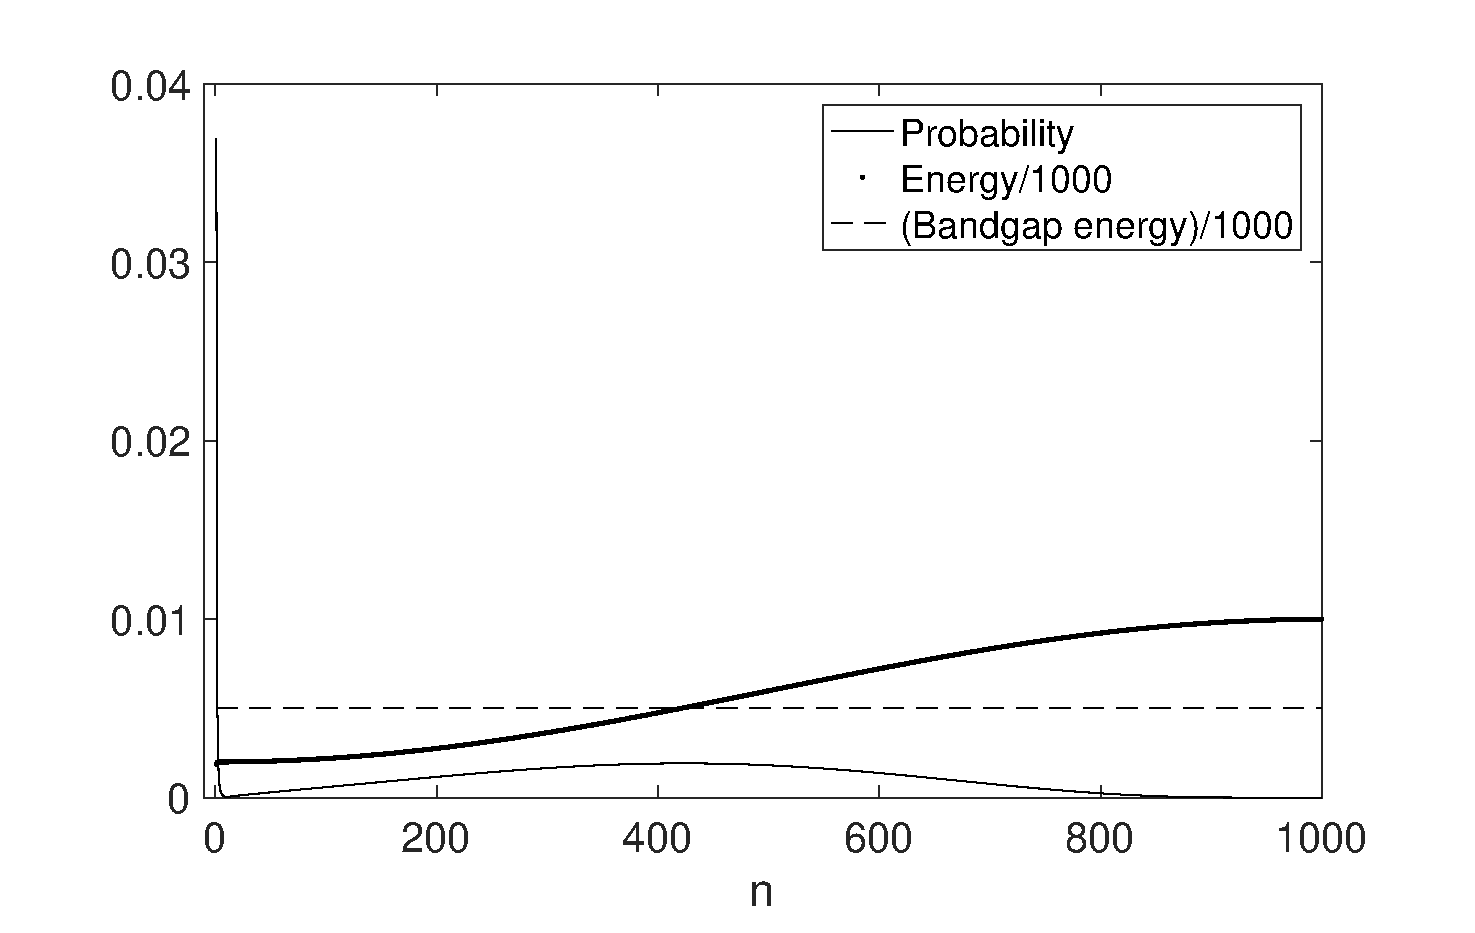
\includegraphics[width=0.7\textwidth]{fig/ExcitonStateU1.eps}
      \caption{The exciton energies and the lowest energy exciton probability plotted as a function of the distance between the electron and holes in unit cells. Shown is also the bandgap energy. For U = 1.} 
      \label{fig:U1}
  \end{figure}
\begin{figure}[!ht]
      \centering
      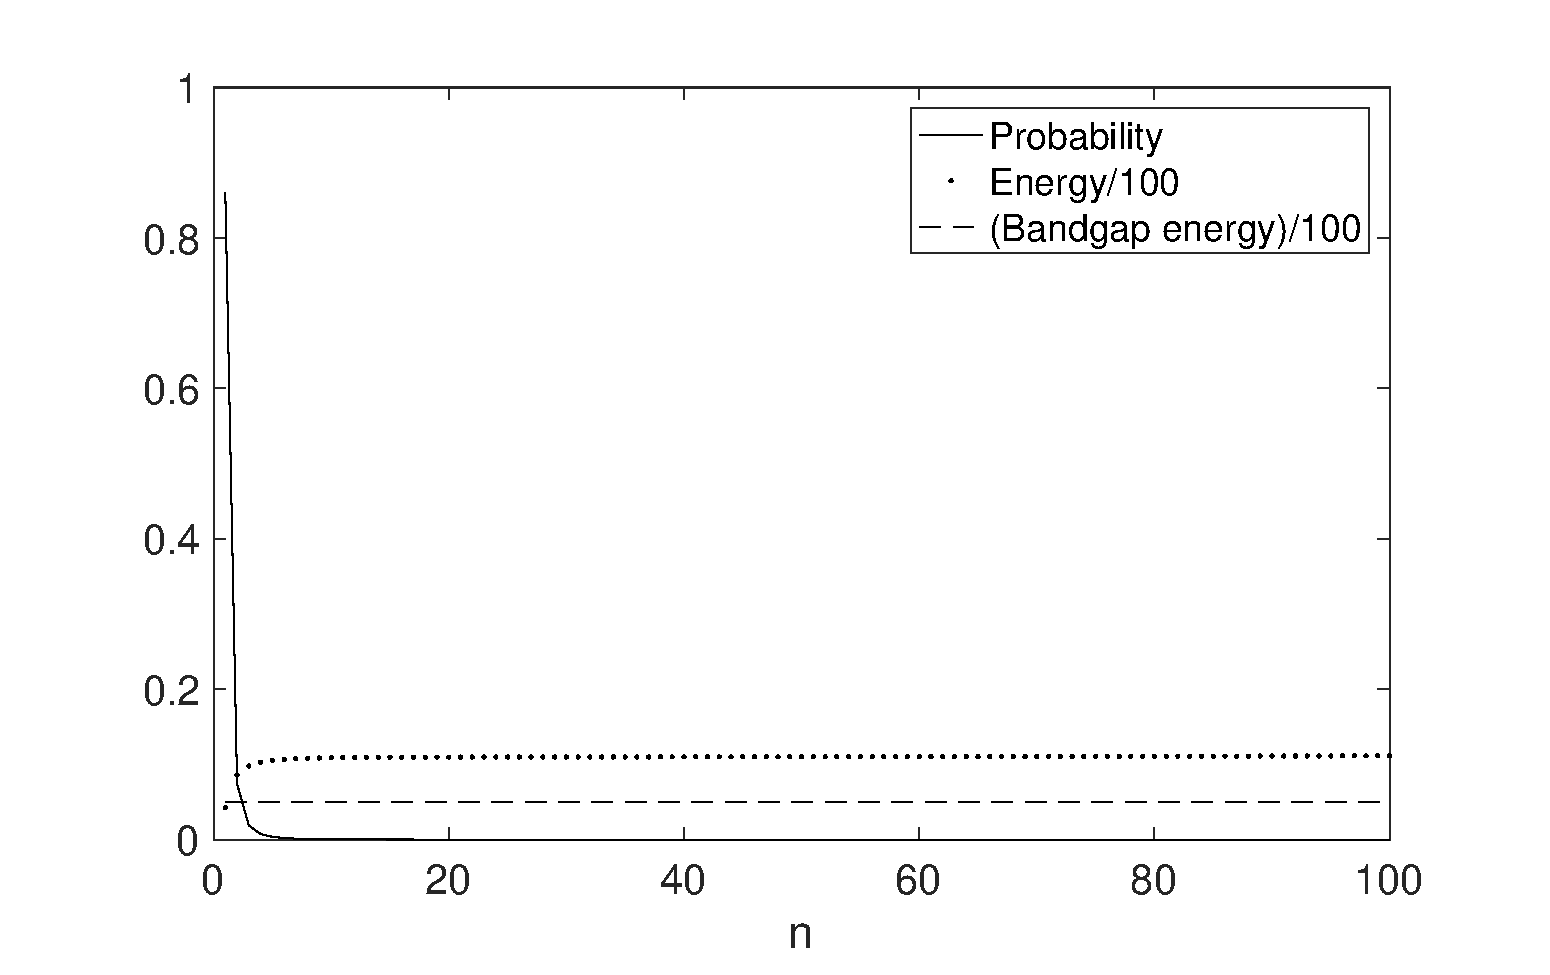
\includegraphics[width = 0.7\linewidth]{fig/ExcitonStateU10.eps}
      \caption{The exciton energies and the lowest energy exciton probability plotted as a function of the distance between the electron and holes in unit cells. Shown is also the bandgap energy. For U = 10.}
      \label{fig:U10}
\end{figure}

\begin{exercise}
Calculate (numerically) and plot the wave function $F_1(n)$ for the lowest lying excition.
\end{exercise}
\begin{solution}

\end{solution}
\newpage \section{The one particle Green function}
\subsection{Spectral properties}



\begin{exercise}
Show that the Green function is only a funciton of the timer difference $t-t'$ such that we can write
\begin{equation}
    G(x,x') = G(r,r';\tau), \quad \tau = t-t'
\end{equation}
\end{exercise}

\begin{solution}
We start with the definition of the Green's funciton given in equation 1 in the problem handout
\begin{equation}\label{eq:generalGreens}
    G(x,x') = -i \theta(t-t') \mel{N}{\{\hat{\Psi}(x),\hat{\Psi}(x')\}}{N}
\end{equation}
And plug in the form of the creation and annihilation operators from the Heisenberg picture $\hat{\Psi}(x) = e^{iHt}\hat{\Psi}(r)e^{-iHt}$, and $\hat{\Psi}^{\dagger}(x) = e^{-iHt}\hat{\Psi}^{\dagger}(r)e^{iHt}$. Plugging this in gives
\begin{equation}
\begin{split}
    G(x,x') \\
    = -i \theta(t-t') \mel{N}{e^{iHt}\hat{\Psi}(r)e^{-iHt}e^{iHt'}\hat{\Psi}^{\dagger}(r)e^{-iHt'} + e^{iHt'}\hat{\Psi}^{\dagger}(r)e^{-iHt'}e^{iHt}\hat{\Psi}(r)e^{-iHt} }{N} \\
    = -i \theta(t-t') e^{iE_0(t-t')} \mel{N}{\hat{\Psi}(r)e^{-iHt}e^{iHt'}\hat{\Psi}^{\dagger}(r) + \hat{\Psi}^{\dagger}(r)e^{-iHt'}e^{iHt}\hat{\Psi}(r) }{N} \\
    = -i \theta(t-t') e^{iE_0(t-t')} \mel{N}{\{\hat{\Psi}(r)e^{iH(t-t')}\hat{\Psi}^{\dagger}(r) + \hat{\Psi}^{\dagger}(r)e^{iH(t-t')}\hat{\Psi}(r)}{N} 
\end{split}
\end{equation}
So that it can now be seen that the greens function only depends on $\tau = t-t'$
\end{solution}



\begin{exercise}
Show that the Fourier transform of the Greens function may be written as
\begin{equation}
    G(r,r';\omega) \equiv \int_{-\infty}^{\infty}\mathrm{e}^{i(\omega+i\eta)\tau}G(r,r';\tau)\mathrm{d}\tau
\end{equation}
\begin{equation}
    G(r,r';\omega) = \sum_i \dfrac{\Psi_{i+}^{QP}(r)\Psi_{i+}^{QP}(r')^{*}}{\omega - \varepsilon_{i+}^{QP} + i\eta} + \sum_i \dfrac{\Psi_{i-}^{QP}(r)\Psi_{i-}^{QP}(r')^{*}}{\omega - \varepsilon_{i-}^{QP} + i\eta}
\end{equation}
where the quasiparticle wave functions and energies have been defined as
\begin{align}\label{eq:QPdef1}
    \Psi_{i+}^{QP}(r) = \mel{N}{\Psi(r)}{N+1,i} \quad , \quad \varepsilon_{i+}^{QP} = E^{i}_{N+1} - E^{0}_{N}  \\
    \Psi_{i-}^{QP}(r) = \mel{N-1,i}{\Psi(r)}{N} \quad , \quad 
    \varepsilon_{i-}^{QP} = E^{0}_{N} - E^{i}_{N-1} \label{eq:QPdef2}
\end{align}
\end{exercise}
\begin{solution}
Starting from equation \ref{eq:generalGreens} and only considering the first term in the anti-commutator and inserting a complete set of eigenstates between the field operators (remembering that this in principle involves all states with any number of particles) we may write
\begin{equation}
    \mel{N}{\Psi(x)\Psi^{\dagger}(x')}{N} = \mel{N}{\Psi(x)\sum_i\ket{N+1,i}\bra{N+1,i}\Psi^{\dagger}(x')}{N}
\end{equation}
where we have used that the annihilation operator must act on an orbital $i$ in a state containing $N+1$ particles, which we label $\ket{N+1,i}$. Here we can use the relation $\Psi(x) = \mathrm{e}^{iHt}\Psi(r)\mathrm{e}^{-iHt}$ to explicitly account for the time dependence.
\begin{equation}
    \mel{N}{\Psi(x)\Psi^{\dagger}(x')}{N} = \sum_i\mathrm{e}^{i(E^{0}_{N} - E^{i}_{N+1})(t-t')}\mel{N}{\Psi(r)}{N+1,i}\mel{N+1,i}{\Psi^{\dagger}(r')}{N}
\end{equation}
Similarly we may obtain an equation for the other term in the anti-commutator, remembering that we here must act on all states containing $N-1$ particles.
\begin{equation}
    \mel{N}{\Psi^{\dagger}(x')\Psi(x)}{N} = \sum_i\mathrm{e}^{i(E^{i}_{N-1} - E^{0}_{N})(t-t')}\mel{N}{\Psi^{\dagger}(r')}{N-1,i}\mel{N-1,i}{\Psi(r)}{N}
\end{equation}
Defining the energies in the exponential and the inner products in accordance with equations (\ref{eq:QPdef1}) and (\ref{eq:QPdef2}) we may write the entire Greens function as
\begin{equation}
    G(r,r';\tau) = -i\theta(\tau)\left(\sum_i \mathrm{e}^{-i\varepsilon_{i+}^{QP}\tau}\Psi_{i+}^{QP}(r)\Psi_{i+}^{QP}(r')^{*} + \sum_i \mathrm{e}^{-i\varepsilon_{i-}^{QP}\tau}\Psi_{i-}^{QP}(r)\Psi_{i-}^{QP}(r')^{*}\right)
\end{equation}
As the quasi-particle field operators are independent of $\tau$ the Fourier transform is simply over the exponential function $\mathrm{e}^{i(\omega + i\eta - \varepsilon_{i\pm}^{QP})\tau}$ bringing the argument into the denominator. The boundaries are now $\tau = 0$ and $\tau \rightarrow \infty$ hence only the $\tau = 0$ term will contribute (ensured by $\eta$). Performing the Fourier transform gives the solution
\begin{equation}
    G(r,r';\omega) = \sum_i \dfrac{\Psi_{i+}^{QP}(r)\Psi_{i+}^{QP}(r')^{*}}{\omega - \varepsilon_{i+}^{QP} +i\eta} + \sum_i \dfrac{\Psi_{i-}^{QP}(r)\Psi_{i-}^{QP}(r')^{*}}{\omega-\varepsilon_{i-}^{QP} + i\eta}
\end{equation}
\end{solution}


\subsection{Non-interacting electrons}
\begin{exercise}
Suppose that we have a non-interacting Hamiltonian $H*0$. The manyparticle state $\ket{N}$ is then an N-particle Slater determinant composed of the N single particle orbitals $\phi_n(r)$ with eigenvalues $\varepsilon_n$. \\
Show that the QP wave functions and energies coincide with single particle orbitals and energies and thus from Eq. (4) the non-interacting Green function becomes
\begin{equation}\label{eq:nonintGreens}
    \begin{split}
        G^0(r,r';\omega) = \sum_{n=1}^N \frac{\phi_n(r) \phi_n^*(r')}{\omega- \varepsilon_n + i \eta} + \sum_{n=N+1}^{\infty} \frac{\phi_n(r) \phi_n^*(r')}{\omega- \varepsilon_n + i \eta}  \\
        = \sum_{n=1}^{\infty} \frac{\phi_n(r) \phi_n^*(r')}{\omega- \varepsilon_n + i \eta}
    \end{split}
\end{equation}
\end{exercise}

\begin{solution}
We start of by evaluating the quasi particle wave functions (eq 6 and 7 in the project handout), where we write the field operators in second quantised form

\begin{equation}
    \begin{split}
        \Psi_{i+}^{QP}(r) = \mel{N}{\sum_n \phi_n c_n}{N+1,i} = \phi_n \\
        \Psi_{i-}^{QP}(r) = \mel{N-1,i}{\sum_n \phi_n c_n}{N} = \phi_n
    \end{split}
\end{equation}
Both of these equations are only non-zero if the annihilation operators remove exactly the i'th state. The top sum only has to evaluate from $N+1$ to infinity, whereas the bottom from 1 to $N$, because otherwise they try to remove electrons that will not bring it to the ground state. Thereby the sums in equation (5) in the problem hand can be changed to run over those exact indices, and the energies in the denominator are just given by the energy associated with the i'th state. Thus the result is obtained by letting $i \rightarrow n$
\begin{equation}
    \begin{split}
        G^0(r,r';\omega) &= \sum_{n=1}^N \frac{\phi_n(r) \phi_n^*(r')}{\omega- \varepsilon_n + i \eta} + \sum_{n=N+1}^{\infty} \frac{\phi_n(r) \phi_n^*(r')}{\omega- \varepsilon_n + i \eta}  \\
        &= \sum_{n=1}^{\infty} \frac{\phi_n(r) \phi_n^*(r')}{\omega- \varepsilon_n + i \eta}
    \end{split}
\end{equation}
\end{solution}

\begin{exercise}
Show that the trace of the non-interacting spectral function
\begin{equation}
\int \mathrm{d}r A^{0}(r,r,\omega)
\end{equation}
is equal to the density of states of the non-interacting Hamiltonian.
\end{exercise}
\begin{solution}
The spectral function is given by equation (13) in the problem handout
\begin{equation}
    A^0(\omega) = - \frac{1}{\pi} \mathrm{Im}(G^0(\omega))
\end{equation}
Plugging in the Green's function as given in equation (18) in the problem handout gives 
\begin{equation}
    A^0(\omega) = \frac{1}{\pi} \sum_n  \pi \delta(\omega- \varepsilon_n) \ket{\phi_n} \bra{\phi_n}
\end{equation}
Where we used the relation $\lim_{\eta \rightarrow 0} \frac{1}{x + i \eta} = \frac{\mathcal{P}}{x} - i \pi \delta(x)$.
\end{solution}
So that the trace is
\begin{equation}
    \int \mathrm{d}r A^0(r,r,\omega) = \int \mathrm{d}r \sum_n \delta(\omega-\varepsilon_n) \ket{\phi_n} \bra{\phi_n}
\end{equation}
Which is the density of states of the non-interacting Hamiltonian.
\subsection{The self-energy}
\begin{exercise}
Show that the non-interacting Greens function satisfies the equation of motion
\begin{equation}\label{eq:EOM}
    \left[i\dfrac{\partial}{\partial \tau} - H^{0}(r)\right]G^{0}(r) = \delta(r-r')\delta(\tau)
\end{equation}
Next, Fourier transform Eq. \ref{eq:EOM} with respect to $\tau$ and verify that it is solved directly by equation (\ref{eq:nonintGreens}).
\end{exercise}
\begin{solution}
Using the definition of the Greens function in real space \eqref{eq:generalGreens} along with the general time derivative of an operator obtained from the Heisenberg picture $i\partial A/\partial t = \comm{A}{H}$ we may write
\begin{equation}
    \dfrac{\partial}{\partial \tau} G^{0}(r,r',\tau)
\end{equation}
\end{solution}

\subsection{On the physical meaning of the QP wave functions}
\begin{exercise}
Use the identity 
\begin{equation}
c_i^{\dagger} = \int \mathrm{d}r\phi_i(r)\Psi^{\dagger}(r)
\end{equation}
to show that the maximum of $\abs{\mel{N+1,i}{c_i^{\dagger}}{N,0}}^2$ is obtained when $\phi_i$ is proportional to $\Psi^{QP}_{i+}$. In other words, the QP wave function $\Psi_{i+}^{QP}$ is the orbital that best mimics the true excited state $\ket{N+1,i}$ of the interacting system in the sense of Eq. (41). Similarly the QP state $\Psi_{i-}^{QP}$ is the orbital that makes $\anni{c}{i} \ket{N,0}$ the best approximation to the excited state $\ket{N-1,i}$
\end{exercise}


\begin{solution}
We plug in the expression for $\crea{c}{i}$ to get
\begin{equation}
    \abs{\mel{N+1,i}{\int \mathrm{d}r\phi_i(r)\Psi^{\dagger}(r)}{N,0}}^2
\end{equation}
The integral and the function $\phi_i(r)$ can be taken outside the inner product, which can furthermore be expanded, so that we get
\begin{equation}
    \int \mathrm{d}r \abs{\phi_i(r)}^2 \mel{N+1,i}{\Psi^{\dagger}(r)}{N,0}\mel{N,0}{\Psi(r)}{N+1,i}
\end{equation}
From the above the quasi particle wave function from equation (6) in the problem handout can be easily recognised, so that
\begin{equation}
    \int \mathrm{d}r \abs{\phi_i(r)}^2 \abs{\mel{N+1,i}{\Psi^{\dagger}(r)}{N,0}}^2
\end{equation}
This is an overlap integral , which clearly is maximised if the two functions overlap, or equivalently one is proportional to the other. \\
\textbf{Note:} What this means is that one can verify how well the model of non interacting electrons works, by checking how well the non interacting wave functions can resemble the quasi particle wave function.
\end{solution}

\begin{exercise}
Next, prove that the norm of the QP wave function is given by
\begin{equation}
    \int \abs{\Psi_{i+}^{QP}(r)}^2 \mathrm{d}r = \mel{N+1,i}{\crea{c}{i}}{N,0}
\end{equation}
with $\crea{c}{i}$ creating an electron in the \textit{normalised} QP state $\ket{\Psi_{i+}^{QP}}$. Consequently the norm of the QP state $\Psi_{i+}^{QP}$ signals to which extent the excited state $\ket{N+1,i}$ can be regarded as a single-particle excitation.
\end{exercise}

\begin{solution}
f
\end{solution}

\subsection{Hartree-Fock approximation}
\begin{exercise}
Apply Wick's theorem to $G_2$ in Eq. (49)
\begin{equation}
    G_2(r,r',r'';t) = -\theta(t) \mel{N}{ \acomm{\crea{\Psi}{}(r'',t)  \anni{\Psi}{}(r,t) \anni{\Psi}{}(r'',t)}{\crea{\Psi}{}(r')}}{N}
    \label{eq:G2}
\end{equation}
and show that 
\begin{equation}
    G_2(r,r',r'';t) = i n(r'') G(r,r',r) - i \rho(r'',r) G(r'',r',t)
\end{equation}
Where $n(r'') = \mel{N}{ \crea{\Psi}{}(r'') \anni{\Psi}{}(r'')}{N}$ is the ground state density and $\rho(r',r) = \mel{N}{ \crea{\Psi}{}(r') \anni{\Psi}{}(r)}{N} $ is the ground state one-particle density matrix.
\end{exercise}


\begin{solution}
To do this we wish to apply Wick's theorem, which for a four operator expectation value can be expressed as
\begin{equation}
    \langle abcd  \rangle = \langle ab \rangle \langle cd \rangle - \langle ac \rangle \langle bd \rangle + \langle ad \rangle \langle bc \rangle
\end{equation}
Writing out \eqref{eq:G2} gives
\begin{equation}
    \begin{split}
        G_2(r,r',r'';t) = -\theta(t) \mel{N}{ \crea{\Psi}{}(r'',t)  \anni{\Psi}{}(r,t) \anni{\Psi}{}(r'',t)\crea{\Psi}{}(r')}{N} \\
         -\theta(t) \mel{N}{\crea{\Psi}{}(r') \crea{\Psi}{}(r'',t)  \anni{\Psi}{}(r,t) \anni{\Psi}{}(r'',t)}{N}
    \end{split}
\end{equation}
The expectation values will only be non zero if they are products of one creation and one annihilation operator, so the above reduces to
\begin{equation}
\begin{split}
    -\theta(t) \mel{N}{ \crea{\Psi}{}(r'',t)  \anni{\Psi}{}(r,t)}{N} \mel{N}{\anni{\Psi}{}(r'',t)\crea{\Psi}{}(r') }{N} \\
    +\theta(t) \mel{N}{ \crea{\Psi}{}(r'',t)   \anni{\Psi}{}(r'',t) }{N} \mel{N}{\anni{\Psi}{}(r,t)\crea{\Psi}{}(r') }{N}\\
    +\theta(t) \mel{N}{\crea{\Psi}{}(r') \anni{\Psi}{}(r,t)}{N}  \mel{N}{\crea{\Psi}{}(r'',t)   \anni{\Psi}{}(r'',t)}{N} \\ -
    \theta(t) \mel{N}{\crea{\Psi}{}(r')   \anni{\Psi}{}(r'',t)   }{N}  \mel{N}{\crea{\Psi}{}(r'',t)  \anni{\Psi}{}(r,t)}{N}
    \end{split}
\end{equation}
Now using the definitions of $n(r'')$ and $\rho(r',r)$ it reduces to
\begin{equation}
\begin{split}
    -\theta(t) \rho(r'',r) \mel{N}{\anni{\Psi}{}(r'',t)\crea{\Psi}{}(r') }{N} \\
    +\theta(t) n(r'') \mel{N}{\anni{\Psi}{}(r,t)\crea{\Psi}{}(r') }{N}\\
    +\theta(t) \mel{N}{\crea{\Psi}{}(r') \anni{\Psi}{}(r,t)}{N}  n(r'') \\ -
    \theta(t) \mel{N}{\crea{\Psi}{}(r')   \anni{\Psi}{}(r'',t)   }{N}  \rho(r'',r)
    \end{split}
\end{equation}
This is recognised as being anticommutators with $\rho$ or $n$ taken outside parentheses,
\begin{equation}
\begin{split}
    - \rho(r'',r) \theta(t)( \mel{N}{\anni{\Psi}{}(r'',t)\crea{\Psi}{}(r') }{N} + \mel{N}{\crea{\Psi}{}(r')   \anni{\Psi}{}(r'',t)   }{N}) \\
    + n(r'') \theta(t) ( \mel{N}{\anni{\Psi}{}(r,t)\crea{\Psi}{}(r') }{N} +\mel{N}{\crea{\Psi}{}(r') \anni{\Psi}{}(r,t)}{N})
    \end{split}
\end{equation}
Plugging in the definition of the Green function given in equation 1 we obtain the right result
\begin{equation}
    G_2(r,r',r'';t) = i n(r'') G(r,r',r) - i \rho(r'',r) G(r'',r',t)
\end{equation}
\end{solution}
\newpage \section{Week 8 \& 9, Newns Anderson model}
\subsection{Section 1; The Green function}
\begin{exercise}
Show that the Fourier transform of the uncoupled Green functions are given by 
\begin{equation}\label{eq:uncoupledGreen}
    G_{ij}^0(\omega) = \frac{\delta_{ij}}{\omega - \varepsilon_i + i \eta}
\end{equation}
Where $i,j \in \{k,a\}$ and $\eta$ is a positive infinitesimal.
\end{exercise}

\begin{solution}
The basis independent form the Green function is given by equation 18 in the note on Green functions:
\begin{equation}
   \hat{G}^0(\omega) = \sum_n \frac{\ket{\phi_n} \bra{\phi_n}}{\omega - \varepsilon_n + i \eta}
\end{equation}
We wish to find the uncoupled Greens functions, hence we operate in the basis of the Greens function with the states spanned in $i,j \in \{k,a\}$. Hence each element can be expressed as the matrix element in the following way:
\begin{equation}
     G_{ij}^0(\omega) = \mel{\phi_i}{\hat{G}^0(\omega)}{\phi_j} = \sum_n \frac{\braket{\phi_i}{\phi_n} \braket{\phi_n}{\phi_j}}{\omega - \varepsilon_n + i \eta}
\end{equation}
And as the set of $\phi_m$ constitutes an orthonormal basis the inner products vanish apart from the cases where $i=n=j$, so that
\begin{equation}
    G_{ij}^0(\omega) = \frac{\delta_{ij}}{\omega - \varepsilon_i + i \eta}
\end{equation}
\end{solution}
\subsection{Section 2; Embedding self-energy}
\begin{exercise}
Use equation (4):
\begin{equation}
    \left[(\omega + i \eta)I - H_0 \right]G^0(\omega) = I
    \label{eq:NonInt}
\end{equation}
and (5):
\begin{equation}
        \left[(\omega + i \eta)I - H \right]G(\omega) = I
        \label{eq:WithInt}
\end{equation}
to show that the full Green function, G, fulfills the Dyson equation
\begin{equation}
    G_{aa}(\omega) = G_{aa}^0(\omega) + G_{aa}^0(\omega) \sum_k V_{ak} G_{ak}(\omega)
\end{equation}
\end{exercise}

\begin{solution}
To solve this we first isolate $H_0$ in \eqref{eq:NonInt}
\begin{equation}
    H_0 = -I (G^0)^{-1} + \left[(\omega + i \eta) \right]I
    \label{eq:HIsolated}
\end{equation}
In equation \ref{eq:WithInt} we write $H = H_0 + V$ and plugin equation \ref{eq:HIsolated}
\begin{equation}
    (G^0)^{-1}G(\omega) - V G(\omega) = I
\end{equation}
Now we multiply by $(G^0)$ from the left, and isolate $G(\omega)$ to obtain
\begin{equation}\label{eq:NA210}
    G(\omega) = G^0 V G(\omega) + G^0
\end{equation}
To find $G_{aa}$ we take the inner product with an a bra and ket.
\begin{equation}
    G_{aa} = \mel{a}{G^{0}}{a} + \mel{a}{G^{0}VG}{a}
\end{equation}
As $G^{0}$ is diagonal in $a$ (see equation \ref{eq:uncoupledGreen}) this term reduces trivially, and the remaining term can be found by introducing several "ones" in a spectral representation.
\begin{align}
    G_{aa} &= G^{0}_{aa} + \mel{a}{G^{0}\sum_b\ket{b}\bra{b}V\sum_k\ket{k}\bra{k}G}{a} \\
    &= G^{0}_{aa} + \sum_{b=a}\sum_k\mel{a}{G^{0}\ket{b}\bra{b}V\ket{k}\bra{k}G}{a}\\
    &= G^{0}_{aa} + \sum_k G^{0}_{aa}V_{ak}G_{ka} \label{eq:NA114}
\end{align}
Where it was used that $G^0$ is non interacting so that a has to equal b.
\end{solution}
\begin{exercise}
Write down a similar equation for $G_{ka}(\omega)$ and show that
\begin{equation}
    \sum_{k}V_{ak}G_{ka}(\omega) = \sum G_{kk}^{0}\abs{V_{ak}}^2G_{aa}(\omega)
\end{equation}
and combine the resulting equation in $G_{ak}$ with the result from $G_{aa}$ to obtain
\begin{equation}
    G_{aa}(\omega) = G_{aa}^{0}(\omega) + G_{aa}^{0}(\omega)\Sigma_{aa}(\omega)G_{aa}(\omega) \quad,\quad \Sigma_{aa}(\omega)=\sum_{k}\dfrac{\abs{V_{ak}}^2}{\omega-\varepsilon_k+i\eta}
\end{equation}
\end{exercise}
\begin{solution}
Starting from \eqref{eq:NA210} we may obtain $G_{ka}$ by taking the matrix element $\mel{k}{G}{a}$ with $k\neq a$.
\begin{equation}
    G_{ka} = G_{ka}^{0} + \sum_{k',k''}\mel{k}{G^{0}}{k'}\mel{k'}{V}{k''}\mel{k''}{G}{a}
\end{equation}
as $G^{0}_{ka} = 0$ for all $k\neq a$ and we only consider $k\neq a$ this term is trivially zero. Similarly $k=k'$ following the same argument, removing the $k'$ sum. As $V_{c,d}$ is only non-zero when either $c=a$ and $d\in k$ or $d=a$ and $c\in k$ we must also have that $k''=a$, further removing the $k''$ sum. Hence
\begin{equation}
    G_{ka} = G_{kk}^{0}V_{ka}G_{aa}
\end{equation}
Multiplying by $V_{ak}$ and summing over $k$, and noting that $V_{ak} = V_{ka}^{*}$ we obtain the solution
\begin{equation}\label{eq:NA119}
    \sum_{k}V_{ka}G_{ka} = \sum_{k}G_{kk}^{0}\abs{V_{ka}}^2G_{aa}
\end{equation}
Defining the self energy as
\begin{equation}\label{eq:NA220}
    \Sigma_{aa}(\omega)=\sum_{k}G^{0}_{kk}\abs{V_{ka}}^2=\sum_{k}\dfrac{\abs{V_{ak}}^2}{\omega-\varepsilon_k+i\eta}
\end{equation}
and inserting \eqref{eq:NA119} in \eqref{eq:NA114} we directly obtain the decoupled Dyson-like equation in $G_{aa}$
\begin{equation}
    G_{aa}(\omega) = G_{aa}^{0}(\omega) + G_{aa}^{0}(\omega)\Sigma_{aa}(\omega)G_{aa}(\omega)
\end{equation}
\end{solution}

\subsection{Section 3; Wideband approximation}

\begin{exercise}
If the metal density of states is approximately constatnt in the region of the localising state and the coupling elements $V_{ak}$ varies only little with $k$, the function $\Delta(\omega) =\Delta$ becomes a constant and the real part of the self-energy vanishes. This is known as the wideband limit. \\
Show that the Green function function in this approximation becomes
\begin{equation}
    G_{aa}(\omega) = \frac{1}{\omega - \varepsilon_a+i \Delta/2}
\end{equation}
Calculate and sketch the spectral function $A_a(\omega) = - \mathrm{Im}G_{aa}(\omega)$
\end{exercise}

\begin{solution}
We start of with equation (8) in the project handout and write the self energy as a sum of a real and an imaginary part.
\begin{equation}
    G_{aa}(\omega) = \frac{1}{\omega - \varepsilon_a-(\mathrm{Re}(\Sigma_{aa}(\omega)) + i \mathrm{Im}(\Sigma_{aa}(\omega)))}
\end{equation}
Now we use that the imaginary part is constant, the real part is zero and equation (9) in the project handout, that states that
\begin{equation}
    \mathrm{Im}(\Sigma_{aa}(\omega)) = -\frac{\Delta}{2}
\end{equation}
Upon plugging this in above the result is obtained
\begin{equation}
        G_{aa}(\omega) = \frac{1}{\omega - \varepsilon_a + i \Delta/2}
\end{equation}

To find the imaginary part of this we multiply both the nominator and denominator with the complex conjugate of the denominator to obtain
\begin{equation}
    G_{aa}(\omega) = \frac{\omega - \varepsilon_a - i \Delta/2}{(\omega - \varepsilon_a)^2 + \Delta^2/4}
\end{equation}
So we obtain
\begin{equation}
    A_a(\omega) = - \mathrm{Im}(G_{aa}(\omega)) = \frac{\Delta/2}{(\omega - \varepsilon_a)^2 + \Delta^2/4}
\end{equation}

\begin{figure}[!ht]
    \centering
    \begin{tikzpicture}[scale=1.2]
            \begin{axis}[
                axis lines=middle,
                ticks=none,
                xmin=-1*pi,xmax=4*pi,
                ymin=-0.1,ymax=1.5,
                xlabel={$\omega$},
                ylabel={$A_a(\omega)$},
                domain=-10000:10000,
                restrict y to domain=-1:2,
                enlargelimits=true
                ]
        % parts:
        \addplot[black,domain=-5.1:13 ,unbounded coords=jump,samples=102] {1/((x-2)^2+1)};
        \draw (0,1) -- (-0.3,1) node[left] {$2/\Delta$};
        \draw (2,0) -- (2,-0.05) node[below] {$\omega=\epsilon_a$};
        
        \end{axis}
    \end{tikzpicture}
    \caption{Illustration of the local density of states for the adsorbed molecule, assuming the self energy to be frequency independent.}
    \label{fig:DOSNEWNS}
\end{figure}
This is a lorentzian shape, that is sketched in figure \ref{fig:DOSNEWNS}. As this is the diagonal elements of the spectral function, it describes local density of states.
\end{solution}






\begin{exercise}
Show that the Green function takes the following form in the time domain,
\begin{equation}
    G_{aa}(t) = -i \theta(t)e^{-i(\varepsilon_0-i \Delta/2)t}
    \label{eq:GreenInTime}
\end{equation}
\end{exercise}


\begin{solution}
The easiest way to do this is to Fourier transform \eqref{eq:GreenInTime}, and show that it gives exactly the Green function in the frequency domain given by equation (11) in the problem handout. So we perform the Fourier transform:
\begin{equation}
    G_{aa}(\omega) = \int_{-\infty}^{\infty} -i \theta(t)e^{-i(\varepsilon_0-i \Delta/2)t} e^{i \omega t} \mathrm{d} \omega
\end{equation}
Note that this time there was no reason to include an infinitesimal imaginary part in the Fourier transform to make it converge, as this is handled by the $i \Delta$. \\
The heavyside function means that the fourier transform only runs from 0 to infinity, so the integral is just
\begin{equation}
    G_{aa}(\omega) = \int_{0}^{\infty} -i e^{-i(\varepsilon_0-i \Delta/2 - \omega)t}  \mathrm{d} \omega = \frac{i}{-i(\varepsilon_0-i \Delta/2 - \omega)} = \frac{1}{\omega - \varepsilon_0  + i \Delta/2 }
\end{equation}
Alternatively this may be obtained by starting from the definition of the Greens function, but with an energy correction to the single particle energies such that $\hat{H}_0\ket{N+1,i} = (\varepsilon_0) + \varepsilon_i + i\Delta/2\ket{N+1,i}$ so that
\begin{equation}
        G_{aa}(t) = -i\theta(t)\mathrm{e}^{i\varepsilon_0 t}\left(\mel{N}{c_a(t)\mathrm{e}^{-i\hat{H}_0 t}c^{\dagger}_a(0)}{N} + \mel{N}{c^{\dagger}_a(t)\mathrm{e}^{i\hat{H}_0 t}c_a(0)}{N}\right)
\end{equation}
remembering that the two terms correspond to the electron and hole, respectively, propagating from time $t=0$ to $t$. Focusing on the electron and the cases of $\varepsilon_i < \varepsilon_f$ and $\varepsilon_i > \varepsilon_f$ separately, we see that the first and second term, respectively, equals zero. The remaining terms have the same sign so that regardless of $\varepsilon_i$ it takes the form:
\begin{equation}
    G_{aa}(t) =  -i\theta(t)\mathrm{e}^{-i(\varepsilon_i+i\Delta/2)t}
\end{equation}
With this result we see that $\abs{G_{aa}(t)}^2$ correspond to the probability of the electron (hole for $\varepsilon_i < \varepsilon_f$) inserted at time $t=0$ is still in the same orbital at time $t$. Before introducing the energy correction $i\Delta/2$ the state would be unchanged as it is non-interacting. Now it decays, corresponding to an inverse life time.
\end{solution}

\subsection{Section 4; Discrete approximation}
\begin{exercise}
Assume that $\Delta(\omega)$ can be represented as a delta function located at $<\varepsilon_k>$ and use a drawing to show that $G_{aa}(\omega)$ can have two distinct poles in this case.
\end{exercise}
\begin{solution}
Using the Kramer-Kronig relations we have that
\begin{equation}
    \Gamma(\omega) = \dfrac{P}{2\pi}\int\dfrac{\delta(\omega'-\omega_k)}{\omega-\omega'}\mathrm{d}\omega' = \dfrac{P}{2\pi} \dfrac{1}{\omega - \omega_k} \propto \dfrac{1}{\omega - \omega_k}
\end{equation}
where $\omega_k = <\varepsilon_k>$ and $P$ is the Cauchy principal value. Looking at $G_{aa}(\omega)$ we have that
\begin{equation}
    G_{aa}(\omega) = \dfrac{1}{\omega - \varepsilon_a - \Gamma(\omega) - i\Delta/2}
\end{equation}
Hence it is clear that we have poles at:
\begin{equation}
    \omega - \varepsilon_a - \Gamma(\omega) = 0
\end{equation}
which is a second order polynomial in $\omega$ with two distinct roots when $(\omega_k + \varepsilon_a)^2 - 2P \geq 0$. This may be illustrated by plotting the straight line $(\omega - \varepsilon_a)$ against $\Gamma(\omega)$ as done in figure \ref{fig:discreteapp}. An alternative approach is to interpret the delta function behaviour as collapsing the sum in \eqref{eq:NA220} so that
\begin{equation}
    \Sigma_{aa}(\omega)= \sum_{k}\dfrac{\abs{V_{ak}}^2}{\omega-\varepsilon_k+i\eta} \approx \dfrac{\abs{V_{ak}}^2}{\omega - <\varepsilon_k> + i\eta}
\end{equation}
Hence the imaginary part of $\Sigma_{aa}$ resembles a delta function in the $\eta \rightarrow 0$ at $\omega = <\varepsilon_k>$.
\begin{figure}
    \centering
    \begin{tikzpicture}[scale=1]
        \begin{axis}[
                axis lines=middle,
                ticks=none,
                xmin=-3,xmax=7,
                x label style={at={(current axis.right of origin)},anchor=north},
                xlabel={$\omega$},
                domain=-10000:10000,
                restrict y to domain=-4:5,
                enlargelimits=true
                ]
            % parts:
            \addplot[black,domain=-3:1.999,samples=102, unbounded coords=jump] {1.7/(x-2)};
            \addplot[black,domain=2.001:10,samples=102, unbounded coords=jump] {1.7/(x-2)};
            \addplot[black,domain=-3:10,samples=102] {(x-1)};
            \draw (1,0.1) -- (1,-0.3) node[below] {$\varepsilon_a$};
            \draw (2,0.1) -- (2,-0.3) node[below] {$\omega_k$};
            \node at (7,5) {$\omega - \varepsilon_a$};
            \node at (2.1,5) {$\Gamma(\omega)$};
            \draw (2.9,1.89) circle (0.2);
            \draw (0.1,-0.9) circle (0.2);
        \end{axis}
    \end{tikzpicture}
    \caption{Schematic illustration of the two poles of $G_{aa}$ for the discrete approximation. The poles are highlighted with circles and are found as the intersection of the two curves $\Gamma(\omega)$ and $\omega-\varepsilon_a$.}
    \label{fig:discreteapp}
\end{figure}
\end{solution}
\subsection{Section 5; Semi-elliptic band}
\begin{exercise}
Show that the imaginary part of the complex function
\begin{equation}\label{eq:semi-ellipse}
    f(z) = a(z/b - \sqrt{[(z+i\eta)/b]^2 - 1})
\end{equation}
regarded as a function of $x = \mathrm{Re}\{z\}$ describes a semi-ellipse of height $a$ and width $2b$. Argue that if $\Delta(\omega)$ us a semi-ellipse of height $a$, width $2b$, $\Gamma(\omega)$ can be obtained from the real part of $f(z)$ and is given by
\begin{equation}\label{eq:Gamma-SE}
    \Gamma(\omega) = \dfrac{a}{2}\left(\omega/b - \theta(\abs{\omega}-b)\mathrm{sign}(\omega)\sqrt{(\omega/b)^2-1} \right)
\end{equation}
\end{exercise}
\begin{solution}
In this case the self energy is represented by \eqref{eq:semi-ellipse}, and thus the imaginary, $\Delta/2$, and real, $\Gamma$, parts are obtained from $f(z)$. Regarding $z$ as real and remembering that we have to work in the limit of $\eta \rightarrow 0$ the only way $f(z)$ can have an imaginary part is when the argument of the square-root is negative. This can readily be seen to be when $\abs{z/b}^2 < 1$. Analysing the imaginary part: $\mathrm{Im}\{f(z)\} \neq 0$ we have that
\begin{equation}
    \mathrm{Im}\{f(z)\} = \begin{cases} -a\sqrt{1 - (z/b)^2} &, z^2 \leq b^2 \\ 0 &, z^2 > b^2 \end{cases}
\end{equation}
This can be recognised as a semi-ellipse of height $a$, width $2b$, and centered at $z = 0$. This means that if $\Delta(\omega)$ is a semi-ellipse with the aforementioned parameters, $\Gamma(\omega)$ can be obtained by the real part of $f(z)/2$ (remembering that $\Delta/2 = \mathrm{Im}\{\Sigma\}$. The real part may be obtained in a similar fashion by analysing the two cases separately
\begin{equation}
    \mathrm{Re}\{f(z)\} = \begin{cases} az/b &, z^2 \leq b^2 \\ az/b - \sqrt{(z/b)^2-1} &, z^2 > b^2 \end{cases}
\end{equation}
Letting $z \rightarrow \omega$ we may alternatively write both functions as continuous functions (in contrast to the piece-wise formulation) through the use of the heavy-side function at $\theta(\abs{\omega} - b)$. Hence
\begin{align}\label{eq:semi_gamma}
    \Gamma(\omega) &= \dfrac{a}{2}\left(\omega/b - \theta(\abs{\omega}-b)\sqrt{(\omega/b)^2-1}\right) \\
    \Delta(\omega) &= -\theta(\abs{\omega}-b)a\sqrt{(\omega/b)^2-1} \label{eq:semi_delta}
\end{align}

\end{solution}

\begin{exercise}
Assume that $\Delta(\omega)$ is a semi-ellipse of width 2, height $a$ and centered at $\omega = 0$. Sketch $\Delta(\omega)$ and $\Gamma(\omega)$. Draw also the straight line $\omega-\varepsilon_a$ for $\epsilon_a = 0$, as well as the spectral function:
\begin{equation}\label{eq:semi_spec}
    A_a(\omega) = -\dfrac{1}{2\pi} \dfrac{\Delta(\omega)}{(\omega - \varepsilon_a -\Gamma(\omega))^2 + (\Delta(\omega)/2)^2}
\end{equation}
in the two cases where $a \gg 1$ (strong coupling) and $a \ll 1$ (weak coupling). Discuss the results and compare with the wide band and discrete approximations.
\end{exercise}
\begin{solution}
The semi-elliptic model allows for a continuous transition from the extremely de-localised bands (wideband approximation), e.g. s-bands, to the extremely localised bands (Discrete model), e.g. molecules and atoms. As a consequence we may be able to model the most pronounced features of e.g. the d-bands which lies somewhere in between the discrete and wideband approximation. We see that for strong coupling, $a \gg 1$ we have two poles in the Greens function as in the case of the discrete approximation, where as for weak coupling $a \ll 1$ the spectral density resembles the shape from the wideband approximation. Hence we are able to model the transition from two distinct poles in the Greens function to one, or none. Figure \ref{fig:semi-ellipse} sketches $\Gamma$, $\Delta$, $A_a$ and $\omega - \varepsilon_a$ making use of equations (\ref{eq:semi_gamma}), (\ref{eq:semi_delta}), and (\ref{eq:semi_spec}), for strong and weak coupling.

\begin{figure}
\begin{minipage}{0.49\textwidth}
    \centering
        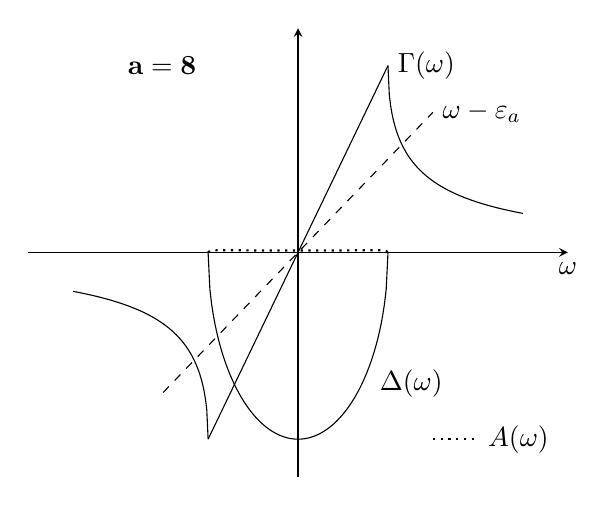
\begin{tikzpicture}[scale=1]
            \begin{axis}[
                    axis lines=middle,
                    ticks=none,
                    xmin=-5,xmax=5,
                    x label style={at={(current axis.right of origin)},anchor=north},
                    xlabel={$\omega$},
                    domain=-2:2,
                    restrict y to domain=-10:10,
                    enlargelimits=true
                    ]
                % Gamma
                \addplot[black,domain=-2:2,samples=102, unbounded coords=jump] {8*0.25*x};
                \addplot[black,domain=-5:-2,samples=102, unbounded coords=jump] {8*(0.25*x + 0.5*sqrt(0.25*x^2-1))};
                \addplot[black,domain=2:5,samples=102, unbounded coords=jump] {8*(0.25*x - 0.5*sqrt(0.25*x^2-1))};
                
                % Delta
                \addplot[black,domain=-2:2,samples=102, unbounded coords=jump] {-8*0.5*sqrt(1-0.25*x^2)};
                
                % omega-epsilon_a
                \addplot[dashed,black,domain=-3:3,samples=102, unbounded coords=jump] {x)};
                
                % Spectral function 
                \addplot[thick,dotted,black,domain=-2:2,samples=102, unbounded coords=jump] {(1/(2*3.14))*(8*0.5*sqrt(1-0.25*x^2))/((x-(8*0.5*0.5*x))^2 + (-8*0.5*sqrt(1-0.25*x^2))^2)};
                
                % LEGEND
                \draw[dotted,thick] (3,-4) -- (4,-4) node[right] {$A(\omega)$};
                \node[right] at (3,3) {$\omega - \varepsilon_a$};
                \node[right] at (2,4) {$\Gamma(\omega)$};
                \node[right] at (1.6,-2.8) {$\Delta(\omega)$};
                \node[right] at (-4,4) {$\mathbf{a = 8}$};
            \end{axis}
    \end{tikzpicture}
\end{minipage}
\begin{minipage}{0.49\textwidth}
\centering
    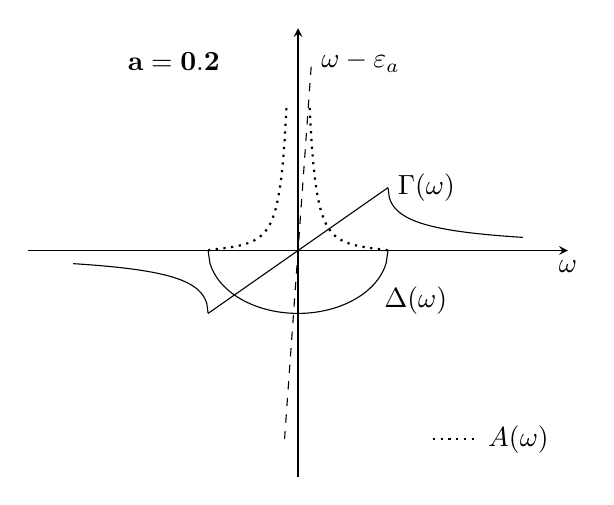
\begin{tikzpicture}[scale=1]
        \begin{axis}[
                axis lines=middle,
                ticks=none,
                xmin=-5,xmax=5,
                x label style={at={(current axis.right of origin)},anchor=north},
                xlabel={$\omega$},
                domain=-2:2,
                restrict y to domain=-0.3:0.3,
                enlargelimits=true
                ]
            % parts:
            % Gamma
            \addplot[black,domain=-2:2,samples=102, unbounded coords=jump] {0.2*0.25*x}; %|x| < b
            \addplot[black,domain=-5:-2,samples=102, unbounded coords=jump] {0.2*(0.25*x + 0.5*sqrt(0.25*x^2-1))}; % x < b
            \addplot[black,domain=2:5,samples=102, unbounded coords=jump] {0.2*(0.25*x - 0.5*sqrt(0.25*x^2-1))}; % x > b
            
            % Delta
            \addplot[black,domain=-2:2,samples=102, unbounded coords=jump] {-0.2*0.5*sqrt(1-0.25*x^2)};
            
            % omega - epsilon_a
            \addplot[dashed,black,domain=-0.3:0.3,samples=102, unbounded coords=jump] {x)};
            
            % Spectral function 
            \addplot[thick,dotted,black,domain=-2:2,samples=102, unbounded coords=jump] {(1/(2*3.14))*(0.2*0.5*sqrt(1-0.25*x^2))/((x-(0.2*0.5*0.5*x))^2 + (-0.2*0.5*sqrt(1-0.25*x^2))^2)};
            
            % LEGEND
            \draw[dotted,thick] (3,-0.3) -- (4,-0.3) node[right] {$A(\omega)$};
            \node[right] at (0.3,0.3) {$\omega - \varepsilon_a$};
            \node[right] at (2,0.1) {$\Gamma(\omega)$};
            \node[right] at (1.7,-0.08) {$\Delta(\omega)$};
            \node[right] at (-4,0.3) {$\mathbf{a = 0.2}$};
        \end{axis}
    \end{tikzpicture}
\end{minipage}
    \caption{Schematic illustration of the semi-elliptic model for strong ($a=8$) and weak ($a=0.2$) coupling, with $\varepsilon_a = 0$ and $b=2$.}
    \label{fig:semi-ellipse}
\end{figure}
\end{solution}

\newpage \section{Image charge}
\subsection{Screened interaction and image charge problem}

\begin{exercise}
We consider a point charge $q$ (we use atomic units so $q$ is measured in units of the elementary charge $e$) located a distance $z$ outside a semi-infinite metal surface. Argue that the potential energy of the point charge is given by
\begin{equation}
    V_{img}(r) = - \frac{q^2}{4z}
\end{equation}
\end{exercise}

\begin{solution}
The conductor will respond to the point charge by screening, which will create an electric field opposing it, so that there is no netto field inside the conductor. This electric field is not very easy to compute, however this problem is the same as another problem. To see this we need to use that the tangential component of the electric field to the surface is continuous across the surface, however since there is no E-field inside the conductor the field lines must point perpendicularly into the surface.


\begin{figure}[!ht]
    \centering
    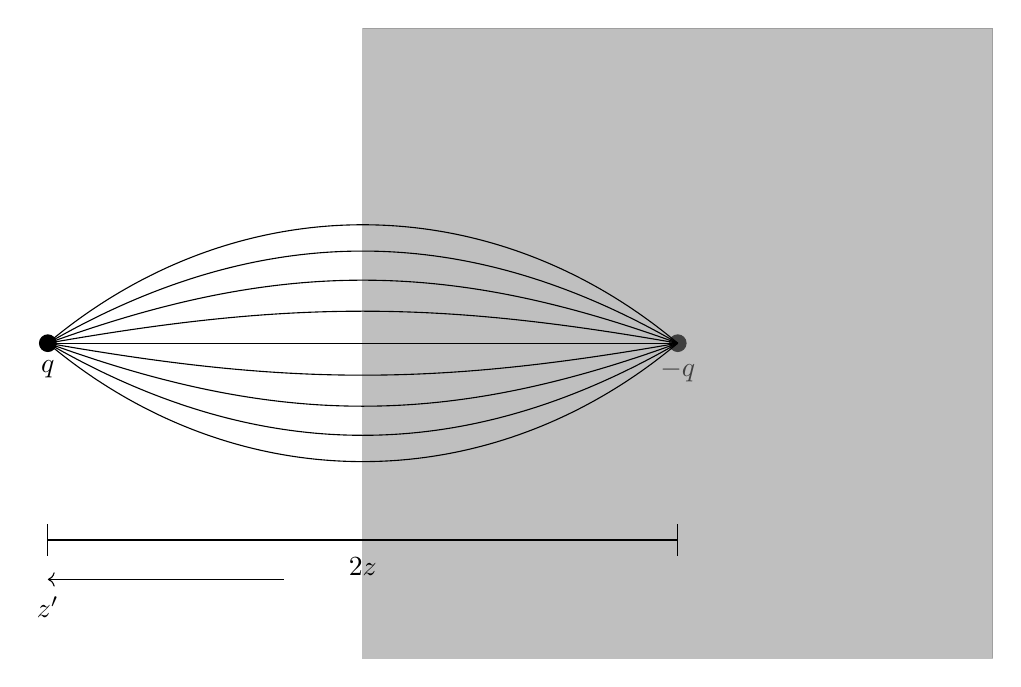
\begin{tikzpicture}
    \filldraw (0,0) circle (3pt);
    \draw (0,-0.1) node[below] {$q$};
    \filldraw (8,0) circle (3pt);
    \draw (8,-0.1) node[below] {$-q$};
    \draw [fill=gray,gray,opacity=0.5] (4,-4) rectangle (12,4); 
    \draw[-] (0,0) to (8,0);
    \draw[-] (0,0) to [out = 40, in=140] (8,0);
    \draw[-] (0,0) to [out = 30, in=150] (8,0);
    \draw[-] (0,0) to [out = 20, in=160] (8,0);
    \draw[-] (0,0) to [out = 10, in=170] (8,0);
    \draw[-] (0,0) to [out = -40, in=-140] (8,0);
    \draw[-] (0,0) to [out = -30, in=-150] (8,0);
    \draw[-] (0,0) to [out = -20, in=-160] (8,0);
    \draw[-] (0,0) to [out = -10, in=-170] (8,0);
    
    \draw[-] (0,-2.5) to (8,-2.5);
    \draw[-] (0,-2.7) to (0,-2.3);
    \draw[-] (8,-2.7) to (8,-2.3);
    \draw (4,-2.6) node[below] {$2z$};
    
    \draw[<-] (0,-3) -- (3,-3);
    \draw (0,-3.1) node[below] {$z'$};
    
    
    \end{tikzpicture}
    \caption{Illustration of the problem, where we instead solve the equivalent problem of the image charge. The conductor above should be imagined to be infinite. The drawn lines illustrates the E-field which are the same regardless if we are looking at the problem with two charges, or the one with one charge and a conductor}
    \label{fig:ImageCharge}
\end{figure}
The force between the two particles in atomic units is given by the Coulombs force
\begin{equation}
    F = - \frac{q^2}{(2z)^2}
\end{equation}
Which means that the potential energy of the point charge is given by
\begin{equation}
    V_{img} = \int_{\infty}^z F \mathrm{d}z' = -\int_{\infty}^z \frac{q^2}{4z} \mathrm{d}z' = -\frac{q^2}{4z}
\end{equation}
Where $z$ is chosen as the upper limit as this is the distance between the point charge and the conductor.
\end{solution}


\begin{exercise}
Argue that the potential at point $r'$ due to the charge density induced in the surface bu a unit charge ($q=e$) point charge at position $r$ is given by
\begin{equation}
    \Delta W_{img}(r,r') = -\frac{1}{2} [(x-x')^2 + (y-y')^2 + (z+z')^2]^{-1/2}
\end{equation}
Note that $\Delta W_{img}(r,r) = V_{img}(r)$ as it should.
\end{exercise}
\begin{solution}

\begin{figure}[!ht]
    \centering
    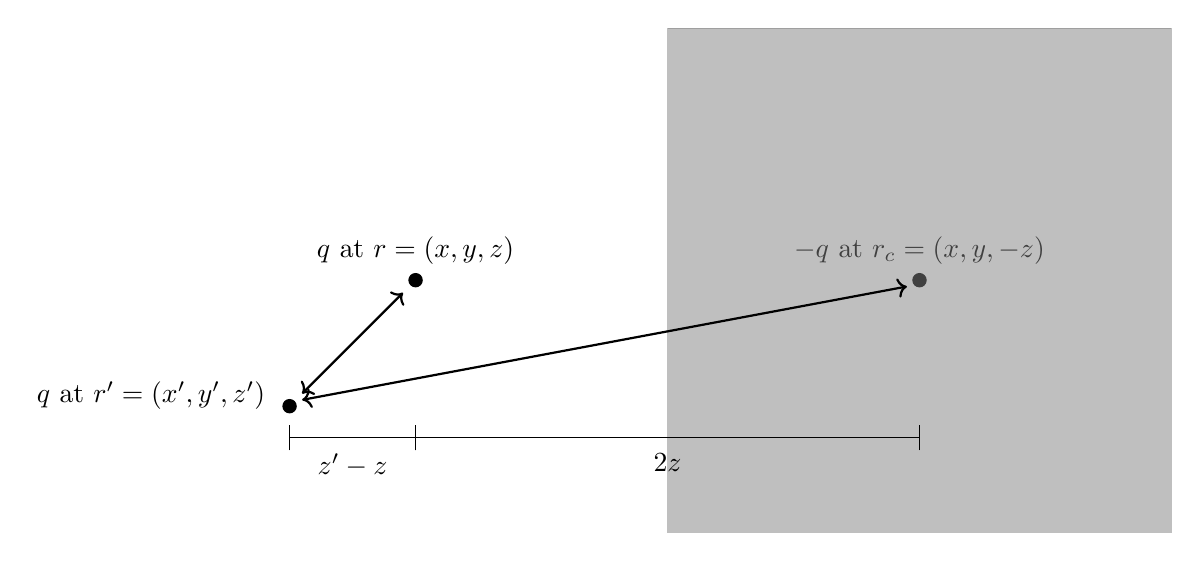
\begin{tikzpicture}[scale=0.8]
    
    
    %Circles
    \filldraw (0,0) circle (3pt);
    \draw (0,0.1) node[above] {$q$ at $r=(x,y,z)$};
    \filldraw (8,0) circle (3pt);
    \draw (8,0.1) node[above] {$-q$ at $r_c = (x,y,-z)$};
    \filldraw (-2,-2) circle (3pt);
    \draw (-4.2,-2.2) node[above] {$q$ at $r'=(x',y',z')$};
    
    %Conductor
    \draw [fill=gray,gray,opacity=0.5] (4,-4) rectangle (12,4); 
   
   % Length scales
    \draw[-] (-2,-2.5) to (0,-2.5);
    \draw[-] (-2,-2.7) to (-2,-2.3);
    \draw[-] (0,-2.7) to (0,-2.3);
    \draw (-1,-2.6) node[below] {$z'-z$};
    
    \draw[-] (0,-2.5) to (8,-2.5);
    \draw[-] (0,-2.7) to (0,-2.3);
    \draw[-] (8,-2.7) to (8,-2.3);
    \draw (4,-2.6) node[below] {$2z$};
    
    %\draw[<-] (0,-3) -- (3,-3);
    %\draw (0,-3.1) node[below] {$z'$};
    %Arrows
    \draw[<->,thick] (-1.8,-1.8) to (-0.2,-0.2);
    \draw[<->,thick] (-1.8,-1.9) to (7.8,-0.1);
    \end{tikzpicture}
    \caption{The problem, now with an extra charge at $r'$}
    \label{fig:ImageCharge2}
\end{figure}
It is straight forward to show by following the same approach as above. There are two contributions for the charge at r', from the charge at r. One direct potential given by
\begin{equation}
    v_{direct} = \frac{q^2}{\sqrt{(x'-x)^2 + (y'-y)^2 + (z'-z)^2}}
\end{equation}
And one from the image charge induced by the charge at r given by
\begin{equation}
\begin{split}\label{eq:806}
    v_{image} = \frac{-q^2}{\sqrt{(x'-x)^2 + (y'-y)^2 + (z'-z +2z)^2}} \\ = \frac{-q^2}{\sqrt{(x'-x)^2 + (y'-y)^2 + (z'+z)^2}}
    \end{split}
\end{equation}
Where $v_{image}$ is exactly $\Delta W_{img}$ as defined in the problem. 
\end{solution}

\begin{exercise}
Show, using the well known relation between the dielectric function and the density response function, that the screened potential induced by the metal surface is given by
\begin{equation}
    \Delta W(r,r') = \int \int v(r,r_1)\chi(r_1,r_2)v(r_2,r')\mathrm{d}r_1\mathrm{d}r_2
\end{equation}
where 
\begin{equation}\label{eq:image_SI}
    W(r,r') = \int \epsilon^{-1}(r,r'')v(r',r)\mathrm{d}r'' \quad \mathrm{and} \quad \Delta W(r,r') = W(r,r') - v(r,r')
\end{equation}
\textbf{NB! Note that the index on the potential differs from the notes}.
\end{exercise}
\begin{solution}
The "well known" relation between the density response function and the dielectric function is given by
\begin{equation}
    \epsilon^{-1}(r,r'') = \delta(r-r'') + \int \dfrac{1}{\abs{r-r_1}}\chi(r_1,r'')\mathrm{d}r_1
\end{equation}
Inserting this in the definition of the induced potential, \eqref{eq:image_SI} right we get
\begin{equation}
    \Delta W(r,r') = \int\delta(r-r'')v(r'',r')\mathrm{d}r'' + \int\int \dfrac{1}{\abs{r-r_1}}\chi(r_1,r'')v(r'',r')\mathrm{d}r_1\mathrm{d}r'' - v(r,r')
\end{equation}
Evaluating the integral over the delta function and re-indexing $r'' \rightarrow r_2$, and rearranging we get 
\begin{equation}
    \Delta W(r,r') = v(r,r') - v(r,r') + \int \int \dfrac{1}{\abs{r-r_1}}\chi(r_1,r_2)v(r_2,r')\mathrm{d}r_1\mathrm{d}r_2
\end{equation}
Finally we recognise the Coulomb term as the potential $v(r,r_1)$ to get:
\begin{equation}
    \Delta W(r,r') =\int\int v(r,r_1)\chi(r_1,r_2)v(r_2,r')\mathrm{d}r_1\mathrm{d}r_2
\end{equation}
\end{solution}

\subsection{Energy levels from the COH-SEX approximation}
\begin{exercise}
Show that when the electron-electron interactions are included at the level of the COH-SEX approximation, the difference between the energy levels of the adsorbed and isolated molecules becomes approximately
\begin{align}
    \varepsilon_H - \varepsilon_H^{gas} &\approx \dfrac{1}{2}\mel{\Psi_H}{\Delta W}{\Psi_H} - (\abs{\Psi_H}^2,\Delta W,\abs{\Psi_{h}^2}) \\
    \varepsilon_L - \varepsilon_L^{gas} &\approx \dfrac{1}{2}\mel{\Psi_L}{\Delta W}{\Psi_L}
\end{align}
where $\Delta W(r,r') = W_{N}(r,r') - W_{F}(r,r')$ ($N$: near, $F$: far) is the difference between the screened interaction with and without the metal surface present and we have introduced the following shorthand notation for a double integral
\begin{equation}
    (f,A,g) = \int \int f(r)A(r,r')g(r') \mathrm{d}r\mathrm{d}r'
\end{equation}
\textbf{Note} that the exercise has the difference in the electron affinity defined as $\varepsilon_L-\varepsilon_H^{gas}$, which is a typo.
\end{exercise}
\begin{solution}
In the static version of the GW approximation, also called the COH-SEX approximation, the self energy takes the form of a non-local one-electron potential, given by:
\begin{equation}
    \Sigma(r,r') = \dfrac{1}{2}[W(r,r') - v(r,r')]\delta(r-r') - \rho(r,r')W(r,r')
\end{equation}
where $\rho$ is the one particle density matrix. 
Denoting the energies by a superscript "far" if the molecules are far away from the metal we may write the ionization potential of the system is given by $\varepsilon_H - \varepsilon_H^{gas}$ where $H$ refers to the HOMO. The QP energy levels and wave functions of the molecules fulfill the QP equation
\begin{equation}
    [H^{0} + \Sigma(\varepsilon_i^{QP})(r,r')]\ket{\Psi_i^{QP}} = \varepsilon_i^{QP}\ket{\Psi_i^{QP}}
\end{equation}
Hence we may find the difference in the ionisation energy of the system with and without the screened interaction by subtracting the QP equations for the two systems, which only differs by the self-energy term
\begin{equation}\label{eq:818}
    [H^{0} + \Sigma(\varepsilon_H)^{N} - H^{0} - \Sigma(\varepsilon_H^{F})]\ket{\Psi_H} = [\Sigma(\varepsilon_H^{N})-\Sigma(\varepsilon_H^{F})]\ket{\Psi_H} = (\varepsilon_H - \varepsilon_H^{gas})\ket{\Psi_H}
\end{equation}
\textbf{Note:} The wave functions may only be assumed to be the same as we are placing the molecule far enough away from the metal surface that we can assume that the orbitals do not overlap, which means the wave functions of the molecule are the same as if there were no metal surface. \\
Taking the expectation value involves a double integral over $r$ and $r'$ as the self-energy is non-local, hence the expectation value from of the Hamiltonian with the self energy may be stated as
\begin{equation}
    \int \mel{\Psi_{H}(r)}{\hat{H}_0\delta(r-r') +\Sigma(r,r')}{\Psi_H(r')}\mathrm{d}r'
\end{equation}
where we have explicitly treated the position dependence. Hence without the self-energy the inner product is defined in it usual form, which shows that $\hat{H}_0$ is diagonal in the $r$ basis. Evaluating equation \ref{eq:818} in the COH-SEX approximation yields:
\begin{equation}\label{eq:image_ionization}
    \begin{split}
        \varepsilon_H - \varepsilon_H^{gas} &\approx \int\dfrac{1}{2}\mel{\Psi_H}{[W_N(r,r')-v_N(r,r') - W_{F}(r,r') + v_{F}(r,r')]\delta(r-r')}{\Psi_H} \\
        &-\mel{\Psi_H}{\rho_{N}(r,r')W_{N}(r,r') -\rho_{F}(r,r')W_{F}(r,r')}{\Psi_H}\mathrm{d}r'
    \end{split}
\end{equation}
Evaluating the first expectation value, with $v_N = v_F$ reduces the expression to
\begin{equation}
    \int\mel{\Psi_H}{[\Delta W_{N}(r,r') - \Delta W_{F}(r,r')]\delta(r,r')}{\Psi_H}\mathrm{d}r' = \mel{\Psi_H}{\Delta W(r,r')}{\Psi_H}
\end{equation}
Analysing the second term in \eqref{eq:image_ionization} shows that we may similarly write it in terms of $\rho_{F}(r,r') = \ket{\Psi_H}\bra{\Psi_H} = \rho_{N}(r,r')$ and $\Delta W(r,r')$ to obtain
\begin{equation}
    \int \int \Psi_H^{*}(r)\Psi_H(r)\Psi_H^{*}(r')\Delta W(r,r') \Psi_H(r') \mathrm{d}r'\mathrm{d}r = \int \int \abs{\Psi_H}^2\Delta W(r,r') \abs{\Psi_H}^2\mathrm{d}r'\mathrm{d}r
\end{equation}
which is alternatively written as $(\abs{\Psi_H}^2,\Delta W(r,r'),\abs{\Psi_H}^2)$. Hence the ionisation energy from \eqref{eq:image_ionization} can be written as
\begin{equation}
    \varepsilon_H - \varepsilon_H^{gas} \approx \dfrac{1}{2}\mel{\Psi_H}{\Delta W}{\Psi_H} - \left(\abs{\Psi_H}^2,\Delta W,\abs{\Psi_H}^2\right)
\end{equation}
The electron affinity can be found from the LUMO state, following the same approach so that the equivalent of \eqref{eq:image_ionization} reads
\begin{equation}
    \varepsilon_L - \varepsilon_L^{gas} \approx \int \dfrac{1}{2}\mel{\Psi_L}{[W_{N}-W_{F}]\delta(r-r')}{\Psi_L} - \mel{\Psi_L}{\rho_N W_{N} - \rho_F W_{F}}{\Psi_L}\mathrm{d}r'
\end{equation}
Again the first term readily simplifies to 
\begin{equation}
    \int\mel{\Psi_L}{[W_{N}-W_{F}]\delta(r-r')}{\Psi_L} \mathrm{d}r'= \mel{\Psi_L}{\Delta W}{\Psi_L}
\end{equation}
The second term needs a more care full treatment as the density operator is given by $\rho_N(r,r') = \ket{\Psi_H(r)}\bra{\Psi_H(r')} = \rho_F(r,r')$, like before, because the only occupied state(s) contributing to the interacting density is the HOMO density. Consequently we have
\begin{equation}\label{eq:image_affinity}
    \int \mel{\Psi_L}{\rho_N W_{N} - \rho_F W_{F}}{\Psi_L}\mathrm{d}r' = \int\int \Psi^{*}_L(r)\Psi_H(r)\Psi^{*}_H(r')\Delta W(r,r')\Psi_L(r')\mathrm{d}r\mathrm{d}r'
\end{equation}
Assuming $\Delta W(r,r')$ to be approximately constant, across the molecule, \eqref{eq:image_affinity} reduces to the
\begin{equation}
    \Delta W \bra{\Psi_L}\ket{\Psi_H}\bra{\Psi_H}\ket{\Psi_L} = 0
\end{equation}
as $\Psi_L$ and $\Psi_H$ are orthogonal. Hence the electron affinity, in the COH-SEX approximation, takes the form
\begin{equation}
    \varepsilon_L - \varepsilon_L^{gas} \approx \mel{\Psi_L}{\Delta W}{\Psi_L}
\end{equation}
\end{solution}

\begin{exercise}
Use the classical model for the image charge potential $\Delta W$ and sketch how the HOMO and LUMO energy levels vary as function of the metal molecule separation.
\end{exercise}
\begin{solution}
Recalling that the quasi-particle energies $\varepsilon_H$ and $\varepsilon_L$ relates to the ionisation potential and electron affinity, respectively, through the definition
\begin{equation}
    \varepsilon_H = E(N) - E(N-1) \quad , \quad \varepsilon_L = E(N+1) - E(N)
\end{equation}
As found in the previous exercise both energies shifts in energies will have a $z^{-1}$ dependence, and in addition the ionisation potential will be shifted by a constant (Again assuming that $\Delta W$ is approximately constant throughout the extend of the molecule). However, the $z^{-1}$ dependence will differ in sign for the two cases. \\
In the HOMO case we are studying the change in energy of the removal energy when we include screening from the metal surface. In this case the test charge (the removed electron) as depicted in figure \ref{fig:ImageCharge2} has the opposite charge and as a consequence the potential from the image charge will go as $+z^{-1}$. \\
In the LUMO case we are studying the change in energy of adding an electron when including screening. In this case the test charge (the added electron) will have the same sign and consequently the potential from the image charge will go as $-z^{-1}$.
\begin{figure}[b!]
    \centering
    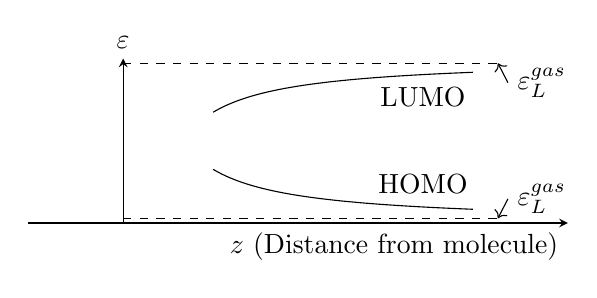
\begin{tikzpicture}
        \begin{axis}[
                axis lines=middle,
                ticks=none,
                y=35,
                xmin=-1,xmax=8,
                x label style={at={(current axis.right of origin)},anchor=north east},
                xlabel={$z$ (Distance from molecule)},
                y label style={anchor=south},
                ylabel={$\varepsilon$},
                domain=-10000:10000,
                restrict y to domain=-4:5,
                enlargelimits=true
                ]
            % parts:
            \addplot[black,domain=1.8:7,samples=102, unbounded coords=jump] {-1/(x)+2};
            \addplot[black,domain=1.8:7,samples=102, unbounded coords=jump] {+1/(x)+0.3};
            %\addplot[black,domain=2.001:10,samples=102, unbounded coords=jump] {1.7/(x-2)};
            %\addplot[black,domain=-3:10,samples=102] {(x-1)};
            \draw[dashed] (0,1.95) -- (7.5,1.95);
            \draw[<-] (7.5,1.95) -- (7.7,1.75) node[anchor=west] {$\varepsilon_L^{gas}$};
            \draw[dashed] (0,0.35) -- (7.5,0.35);
            \draw[<-] (7.5,0.35) -- (7.7,0.55) node[anchor=west] {$\varepsilon_L^{gas}$};
            %\draw (2,0.1) -- (2,-0.3) node[below] {$\omega_k$};
            \node at (6,1.6) {LUMO};
            \node at (6,0.7) {HOMO};
            %\node at (2.1,5) {$\Gamma(\omega)$};
            %\draw (2.9,1.89) circle (0.2);
            %\draw (0.1,-0.9) circle (0.2);
        \end{axis}
    \end{tikzpicture}
    \caption{Schematic illustration of the change in the ionisation potential (HOMO) and electron affinity (LUMO) when including screening from a nearby metal surface, calculated using the COH-SEX approximation with the classical screened potential (\eqref{eq:806}).}
    \label{fig:image_energies}
\end{figure}
\end{solution}
\newpage \section{Correlation energies from the Random Phase Approximation}
\subsection{The adiabatic connection}
\begin{exercise}
Show the Hellman-Feynman theorem.
\begin{equation}
    \dv{\lambda}\mel{\Psi_{\lambda}}{\hat{A}_{\lambda}}{\Psi_{\lambda}} = \mel{\Psi_{\lambda}}{\dv{\lambda}\hat{A}_{\lambda}}{\Psi_{\lambda}}
\end{equation}
(Hint: Use that $\braket{\Psi_{\lambda}}{\Psi_{\lambda}}=1$ for all $\lambda$) 
\end{exercise}

\begin{solution}
Upon applying the operator on both sides we obtain
\begin{equation}
        \dv{\lambda}\mel{\Psi_{\lambda}}{a_{\lambda}}{\Psi_{\lambda}} = \mel{\Psi_{\lambda}}{\dv{\lambda}a_{\lambda}}{\Psi_{\lambda}}
\end{equation}
$a_{\lambda}$ can be moved outside the integral, and so can the derivative in the second term as the integral is not over $\lambda$, thus
\begin{equation}
    \dv{\lambda} a_{\lambda} = \dv{\lambda} a_{\lambda}
\end{equation}
Where the hint was used, thus it is shown.
\end{solution}



\end{document}
